\chapter{The Large Hadron Collider}
\label{ch:lhc}
The Large Hadron Collider (LHC) is a 27\unit{km} two-ring superconducting
proton accelerator and collider located at CERN, spanning the border between
France and Switzerland.  At design specifications, the LHC will collide
protons at a center-of-mass energy of 14\TeV and instantaneous
luminosity $10^{34} \unit{cm}^{-2} \unit{s}^{-1}$.
\begin{table*}
\centering
 \caption{Comparison between LHC design parameters and achieved
   parameters in 2012 and 2015.
 \label{tab:LHCparameters}}
\resizebox{\textwidth}{!}{
\begin{tabular}{|l|c|c|c|c|}
\hline 
Parameter & Unit & \textbf{Design} & \textbf{Acheived (2012)} & \textbf{Acheived (2015)} \\\hline
\multicolumn{5}{|c|}{\textbf{Beam Data}}\\\hline
Proton energy & [GeV] & 7000 & 4000 & 6500 \\\hline
Relativistic gamma factor $\gamma_r$ & & 7461 & 4263 & 6928 \\\hline
Number of particles per bunch $N_b$ & & $1.15\times10^{11}$ &
                                                        $1.6-1.7\times10^{11}$ & $1.15\times10^{11}$ \\\hline
Number of bunches $n_b$ & & 2808 & 1374 & 2244 \\\hline
Bunch spacing & [ns] & 25 & 50 & 25 \\\hline
%Longitudinal emittance ($4\sigma$) & [eV s] & 2.5 & & \\\hline
Transverse normalized emittance $\varepsilon_n$& [$\mu$m rad] & 3.75
                                   &2.5& $\geq2.7$\\\hline
Circulating beam current & [A] & 0.582 & 0.369&\\\hline
Stored energy per beam & [MJ] & 362 & 140 &\\\hline
\multicolumn{5}{|c|}{\textbf{Peak Luminosity Related Data}}\\\hline
$\beta^{\ast}$ at IP1 and IP5 & [m] &0.55 & 0.6 & 0.8 \\\hline
RMS bunch length $\sigma_z$& [cm] & 7.55 & $\geq 9$ &\\\hline
RMS beam size at IP1 and IP5 $\sigma^{\ast}$ & [$\mu$m] & 16.7 & 19 &\\\hline 
Half crossing angle at IP1 and IP5 $\theta_c/2$& [$\mu$rad] & $\pm142.5$ &
                                                               $\pm145.0$ & $\pm145.0$\\\hline
Geometric luminosity reduction factor $F$ & &0.836 & &\\\hline
Peak luminosity in IP1 and IP5 & [cm$^{-1}$s$^{-1}$] &
                                                       $1.0\times10^{34}$ & $7.7\times10^{33}$ & $5.2\times10^{33}$ \\\hline
Max. mean number of events per bunch crossing& & 19 & 40 & 17 \\\hline
\end{tabular}
}
\end{table*}

The LHC is the pinnacle of the accelerator
complex at CERN, pictured in Fig.~\ref{fig:LHCComplex}.  To accelerate
protons to a beam energy of 6.5\TeV in the LHC, a chain of smaller
accelerators are needed. Starting from bottle of hydrogen gas,
electrons are stripped from the hydrogen atoms by an electric field
and the resulting protons enter the Linac 2, which accelerates the
protons to 50\MeV. Subsequently, the Proton Synchrotron Booster (PSB), Proton Synchrotron (PS), and the
Super Proton Synchrotron (SPS) accelerate the protons to 1.4\GeV, 25\GeV, and 450\GeV, respectively, before they are finally injected
into the two LHC rings as counter-rotating beams.

\begin{figure}\centering
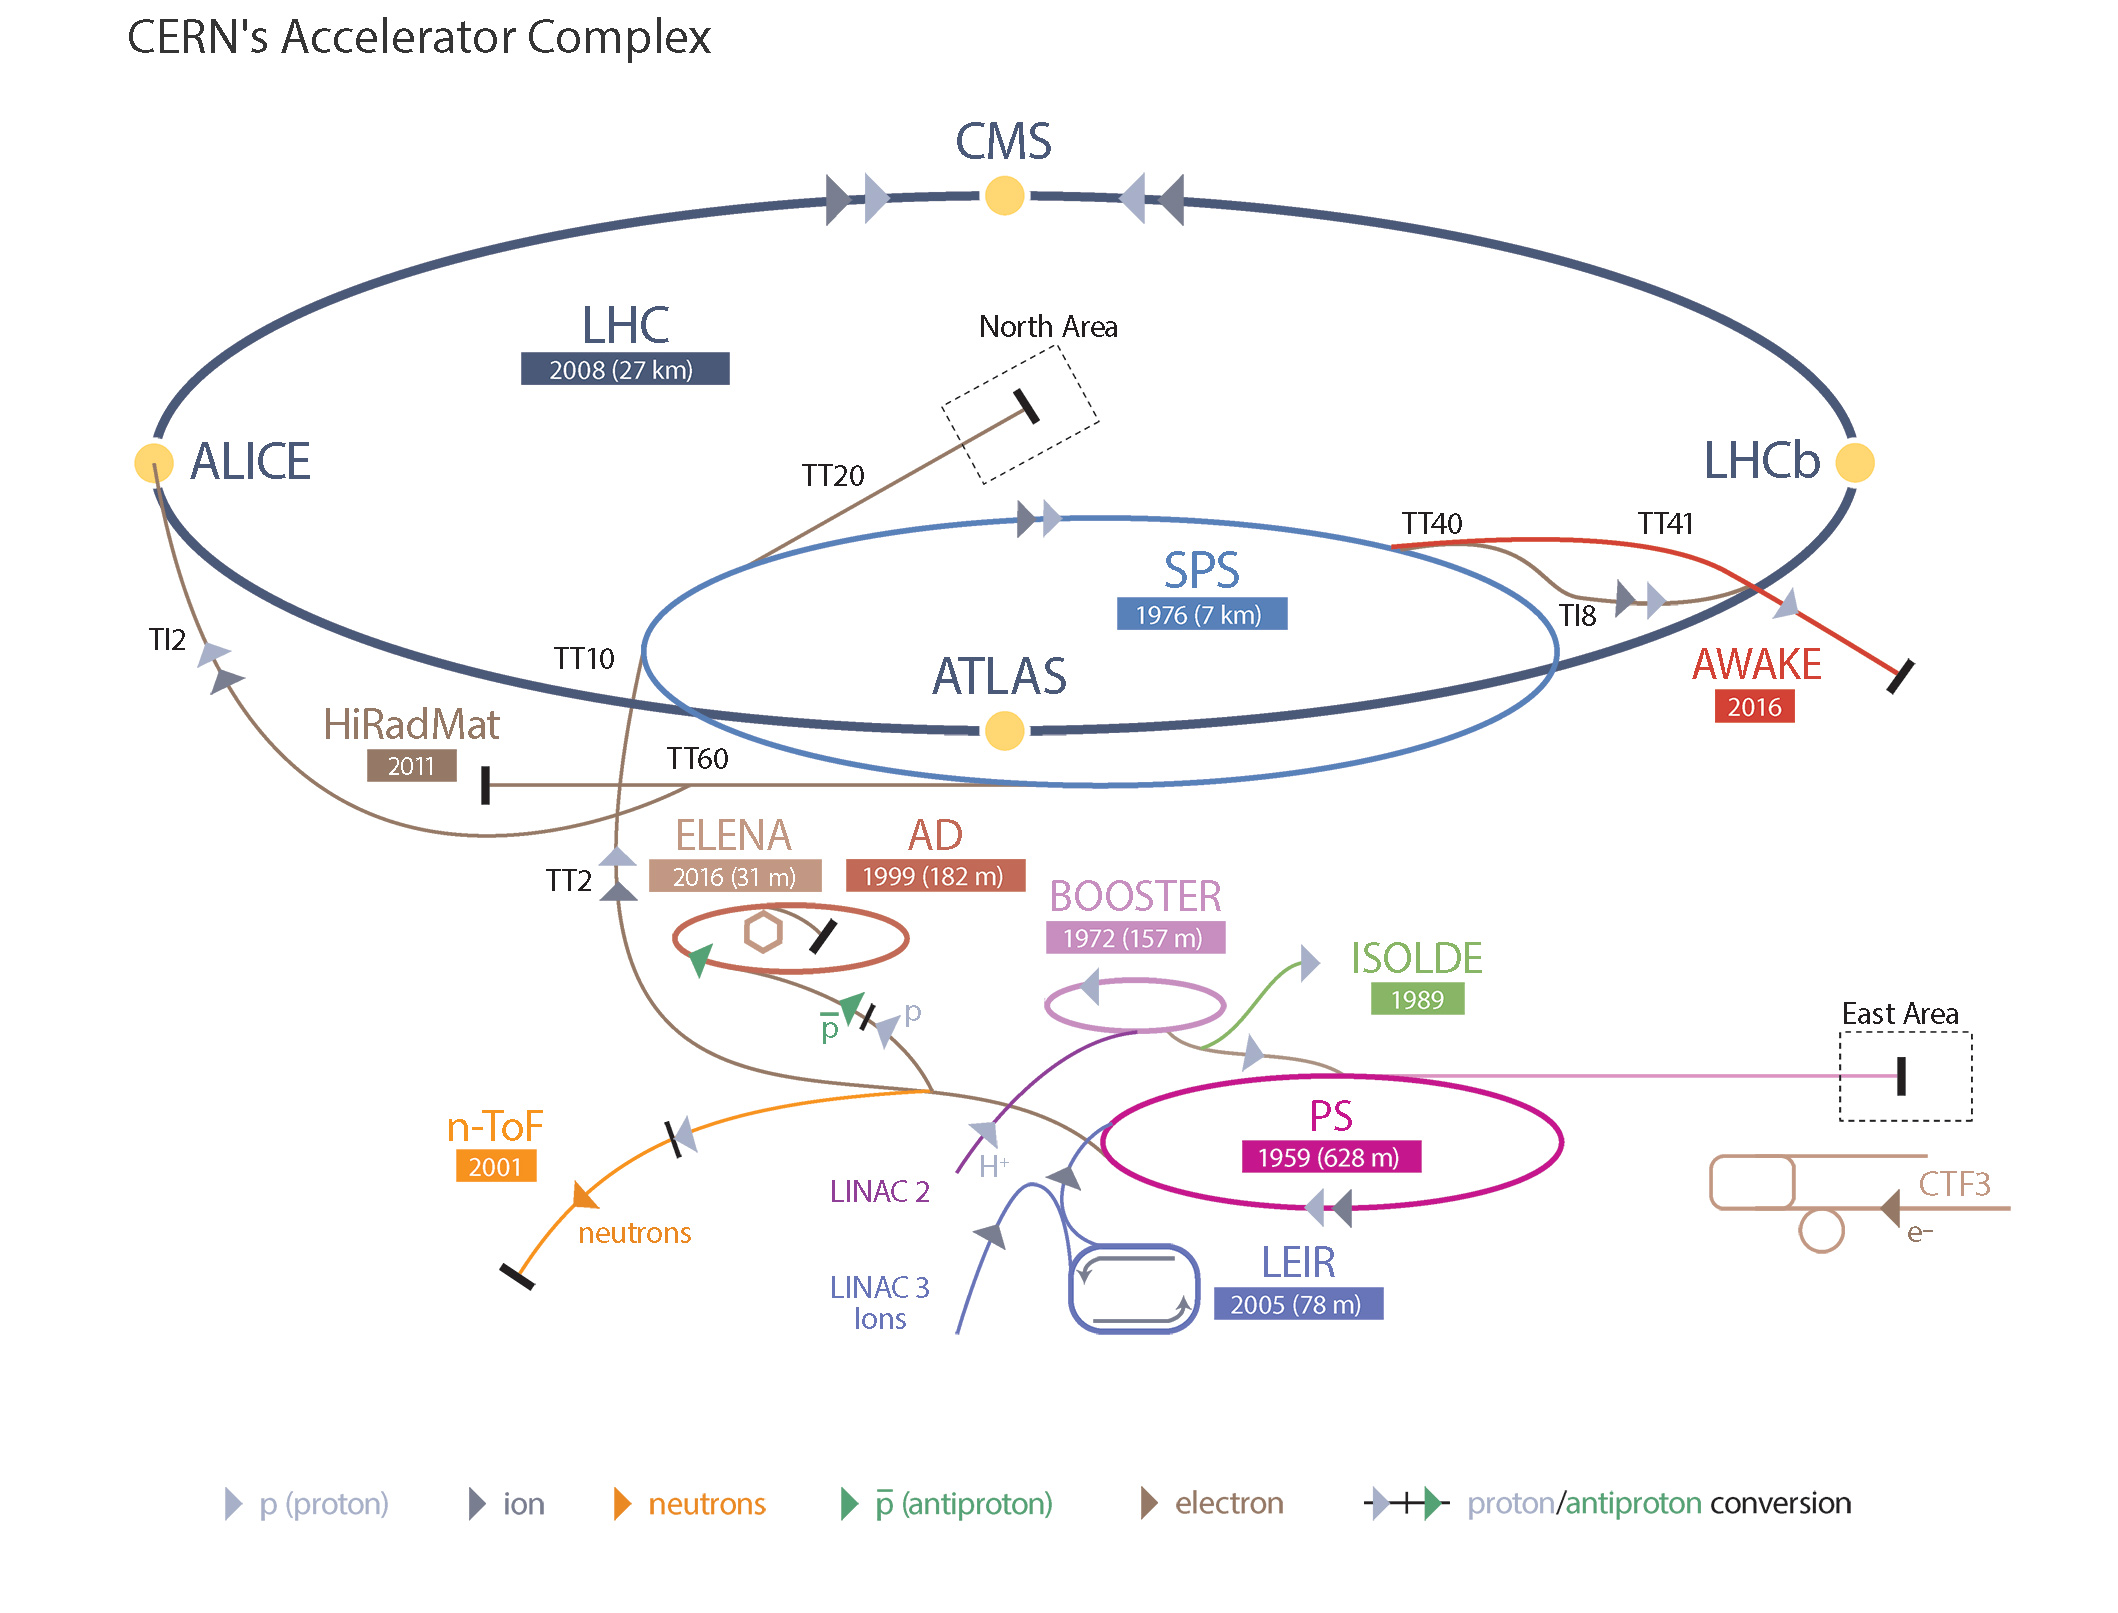
\includegraphics[width=.9\textwidth]{figs/cms/LHC_default.jpg}
\caption{CERN's accelerator complex.\label{fig:LHCComplex}}
\end{figure}

One of the main features influencing the design of the LHC is the re-use of the
existing 26.7\unit{km} tunnel from the Large Electron Positron collider (LEP), which is
comprised of eight crossing points (or arcs) and eight straight sections for
RF cavities. The tunnel in the arc sections has an internal diameter of 3.7\unit{m}. Due to the limited available space, two completely separate
proton rings would be extremely difficult to install.  magnets
would be  difficult to fit in which makes the twin-bore magnet design proposed by John
Blewett in 1971~\cite{Blewett:1068131} ideal due to its
``two-in-one'' use of the limited space. A cross-section of the main superconducting
dipole magnet is shown in \ref{fig:LHCDipole}.

\begin{figure}\centering
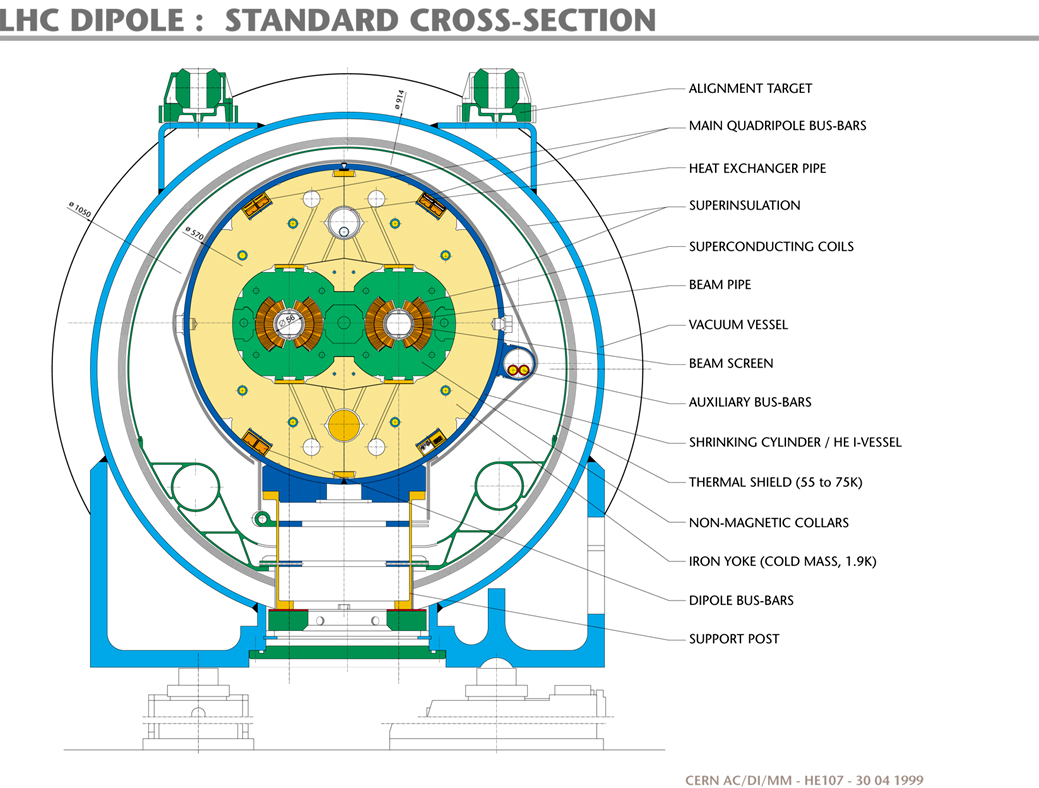
\includegraphics[width=.9\textwidth,clip=true,viewport=0 20 680 550]{figs/cms/lhc-pho-1999-172.jpg}
\caption{Cross-section of the LHC dipole magnet.\label{fig:LHCDipole}}
\end{figure}

The observed number of events $N_{\mathrm{exp}}$ is the product of the cross
section of interest $\sigma_{\mathrm{exp}}$ and the time integral of
the instantaneous luminosity,
\begin{equation}
N_{\mathrm{exp}}  =\sigma_{\mathrm{exp}}\int \mathscr{L}(t)dt ~.
\end{equation}
The instantaneous luminosity depends on the beam parameters and
can be written for a Gaussian beam distribution as~\cite{LHCMachine}:
\begin{equation}
\mathscr{L} =
\frac{N_b^2n_bf_{\mathrm{rev}}\gamma_r}{4\pi\varepsilon_n\beta^{\ast}}F~,
\label{eqn:instlumi}
\end{equation}
where $N_b$ is the number of particles per bunch, $n_b$ the number
of bunches per beam, $f_{\mathrm{rev}}$ the revolution frequency,
$\gamma_r$ the relativistic gamma factor, $\varepsilon_n$ the
normalized transverse beam emittance, $\beta^{\ast}$ the beta function
at the collision point, and $F$ the geometric luminosity reduction
factor due to the crossing angle at the interaction point (IP):
\begin{equation}
F=\left(1+\left(\frac{\theta_c\sigma_z}{2\sigma^{\ast}}\right)^2\right)^{-1/2}~,
\label{eqn:F}
\end{equation}
where $\theta_c$ is the full crossing angle, $\sigma_z$ is the RMS
bunch length, and $\sigma^{\ast}$ is the RMS bunch size.

The integrated luminosity delivered by the LHC to the CMS experiment
versus time for $2010-2016$ is shown in Fig.~\ref{fig:IntLumi20102016}.

\begin{figure}\centering
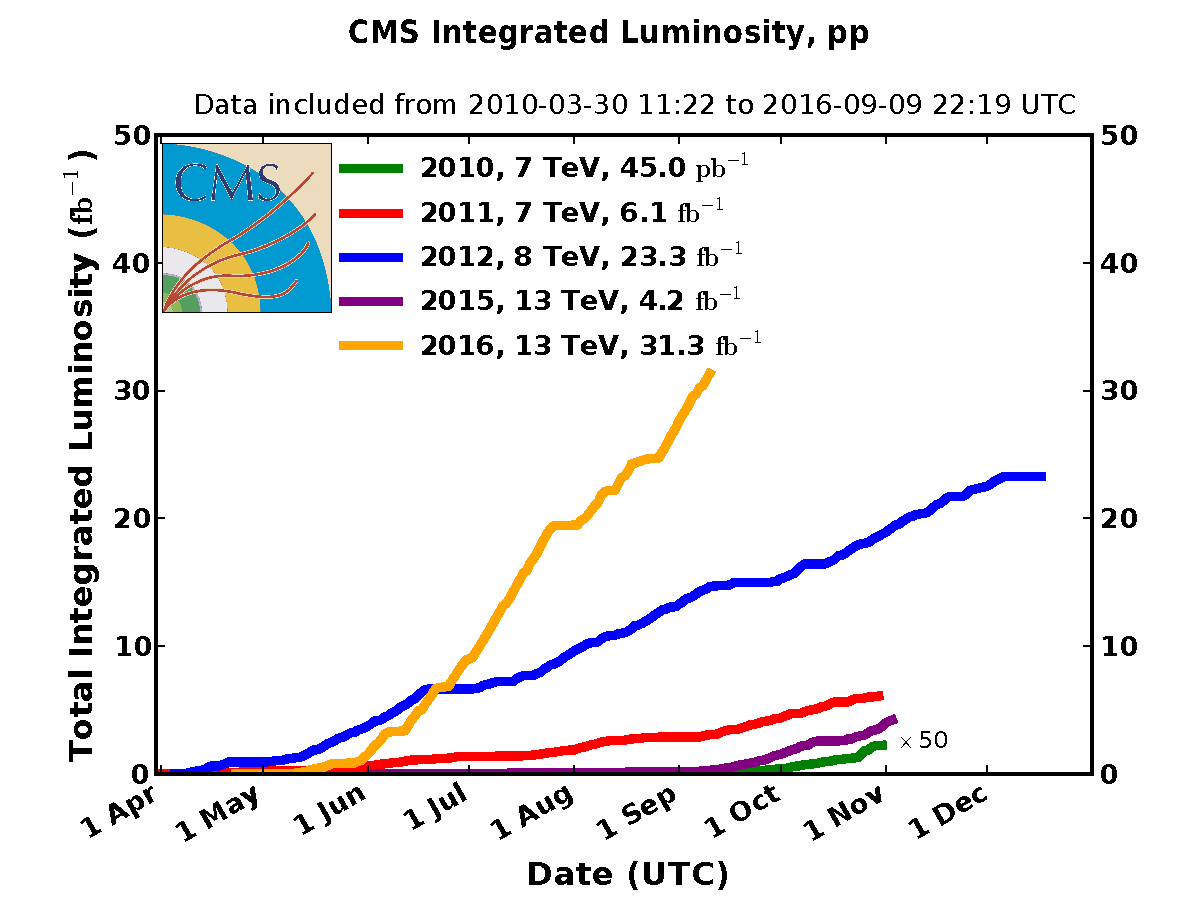
\includegraphics[width=.9\textwidth]{figs/cms/int_lumi_cumulative_pp_2.pdf}
\caption{Cumulative luminosity versus day delivered to CMS during
  stable beams for $\Pp\Pp$  collisions. This is shown for 2010 (green), 2011
  (red), 2012 (blue), 2015 (purple) and 2016 (orange)
  data-taking.\label{fig:IntLumi20102016}}
\end{figure}


\chapter{The CMS Experiment}
\label{ch:cms}
The Compact Muon Solenoid (CMS) detector is a multi-purpose detector
conceived to study proton-proton (and lead-lead) collisions produced
by the Large Hadron Collider (LHC) at CERN~\cite{Adolphi:2008zzk}.

The ultimate goals of the LHC physics programme are to elucidate the nature of
electroweak symmetry breaking and search for evidence of new symmetries, new
forces, or new constituents of matter that could pave the way toward a
unified theory beyond the standard model. There are several detector
and readout requirements for CMS to meet these goals:
\begin{itemize}
\item Good muon identification and momentum resolution over a wide
  range of momenta, good dimuon mass resolution ($\approx 1\%$ at 100
  \GeV), and the ability to unambiguously determine the charge of muons
  with $p<1 \TeV$. See Sec.~\ref{sec:muon};
\item Good charged particle momentum resolution and reconstruction
efficiency in the inner tracker. Efficient triggering and offline
identification of $\Pgt$ leptons and \PQb-jets, requiring pixel
detectors close to the interaction region. See Sec.~\ref{sec:tracker};
\item Good electromagnetic energy resolution, good diphoton and
  dielecron mass resolution ($\approx 1\%$ at 100 \GeV), wide
  geometric coverage, $\pi^0$ rejection, and efficient photon and
  lepton isolation at high luminosities. See Sec.~\ref{sec:ecal};
\item Good missing-transverse-energy and dijet-mass resolution,
  requiring hadron calorimeters with hermetic geometric coverage and
  fine lateral segmentation. See Sec.~\ref{sec:hcal};
\item Fast online event selection process (\emph{trigger}) to reduce the rate from $10^9$ inelastic collision
  events per second to $\lesssim1000$ events per second for storage
  and subsequent analysis. See Sec.~\ref{sec:trigger};
\item Infrastructure for the alignment and calibration of the detector. See Sec.~\ref{sec:alca}.
\end{itemize}
The design of CMS, pictured in Fig.~\ref{fig:CMSperspective} and detailed
in the following sections, meets these requirements. Each detector subsystem is
integral to the performance of CMS as a whole and is specialized to a
particular class of particles, as seen in Fig.~\ref{fig:CMSslice}: the silicon
tracker measures the tracks of charged particles, the electromagnetic
calorimeter measures the energy of electrons and photons, the hadron calorimeter measures the
energy of charged and neutral hadrons, the
superconducting solenoid bends the tracks of charged particles to
allow for a precise momentum measurement, and the muon detectors
identify and measure the momentum of muons.

%The central feature of the CMS detector is a
%superconducting solenoid of 6\unit{m} internal diameter, providing a
%magnetic field of 3.8\unit{T}. Within the superconducting solenoid
%volume are a silicon pixel and a silicon strip tracker, a
%lead-tungstate crystal electromagnetic calorimeter, and a
%brass/scintillator hadron calorimeter, each composed of a barrel and
%two endcap sections. Muons are measured in gas-ionization detectors
%embedded in the magnet steel flux-return yoke outside the
%solenoid. Extensive forward calorimetry complements the coverage
%provided by the barrel and endcap detectors. Jets and leptons are
%econstructed within the pseudorapidity region $\abs{\eta}<3$, covered by the
%electromagnetic and hadron calorimeters. Muons are reconstructed with
%$\abs{\eta}<2.4$. Events are selected by a two-level trigger system. The first level (L1) is based on a hardware
%filter, followed by a software-based high-level trigger (HLT). 

\begin{figure}\centering
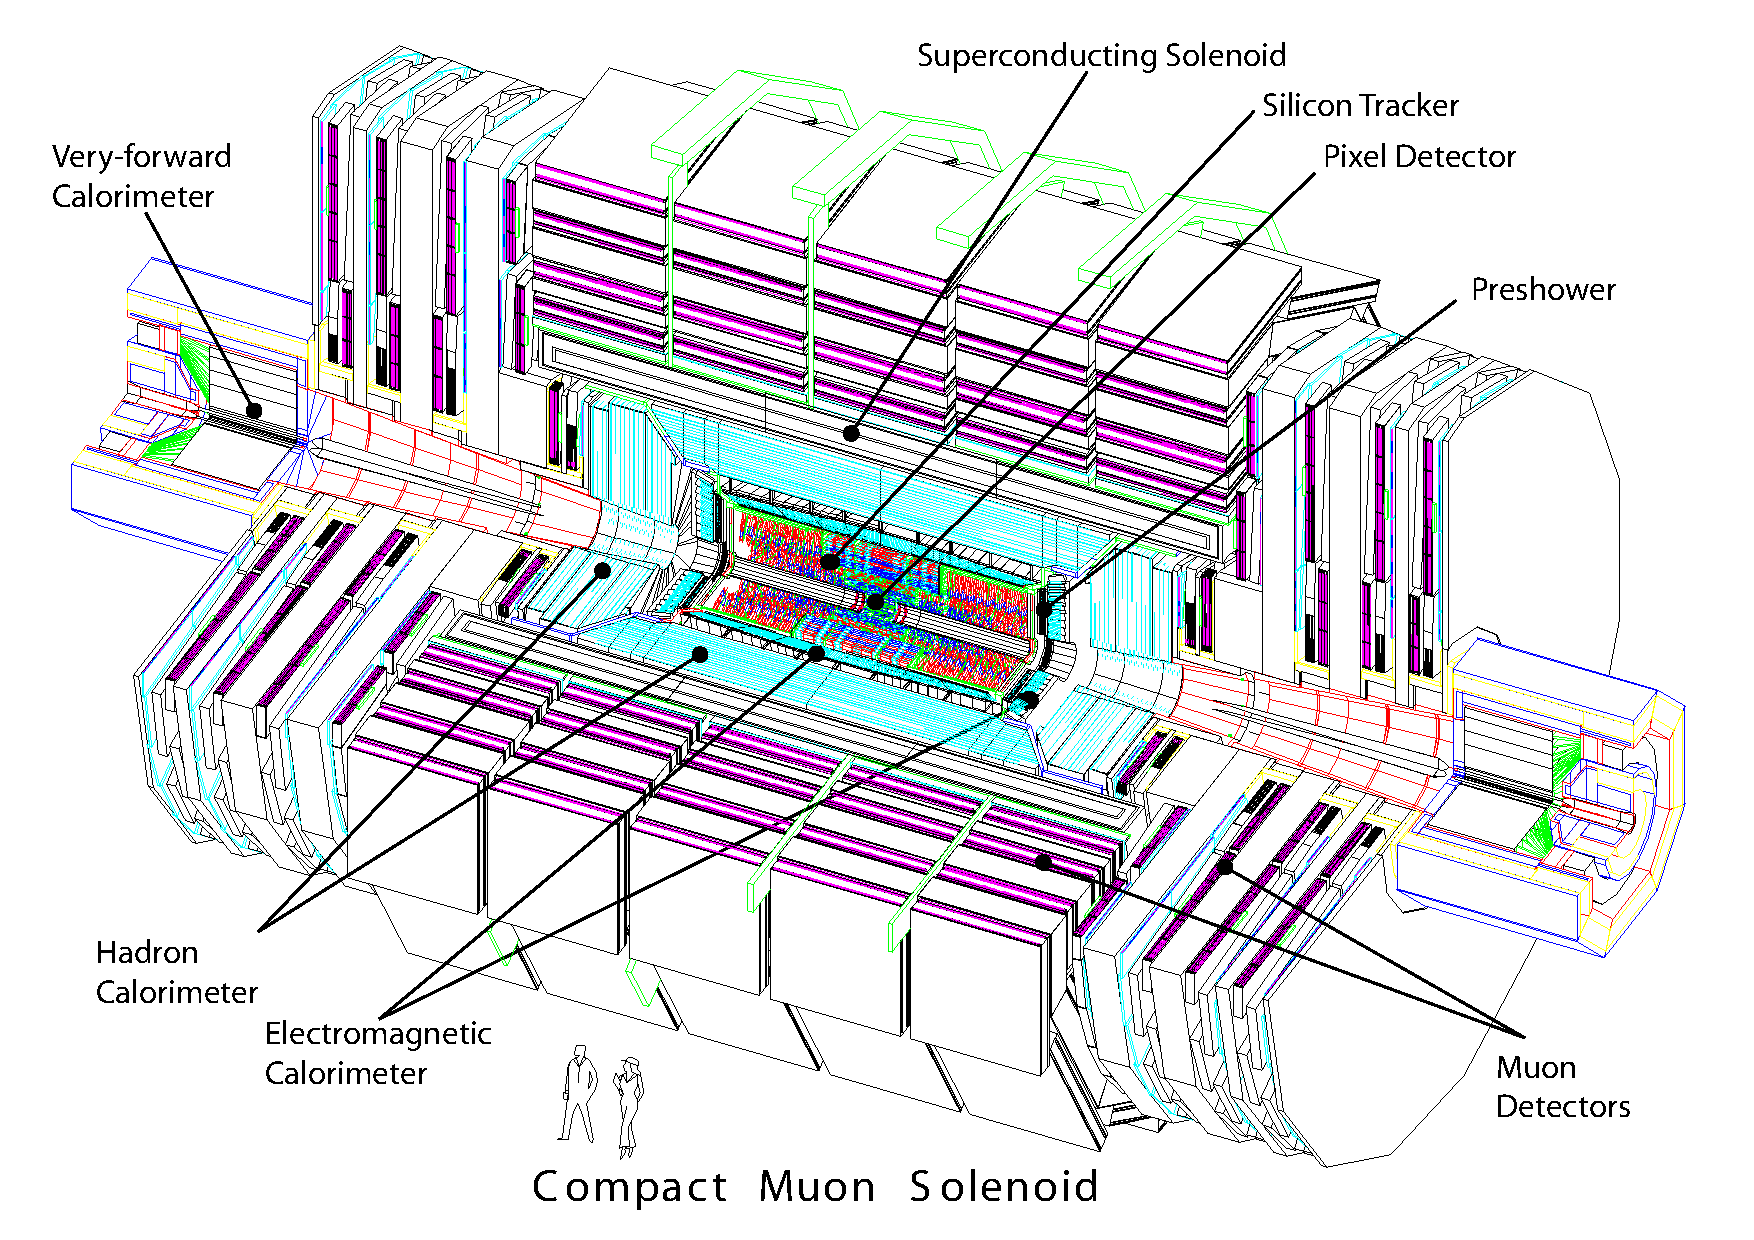
\includegraphics[width=.9\textwidth]{figs/cms/Figure_001-002.pdf}
\caption{Perspective view of the CMS detector.\label{fig:CMSperspective}}
\end{figure}

\begin{figure}\centering
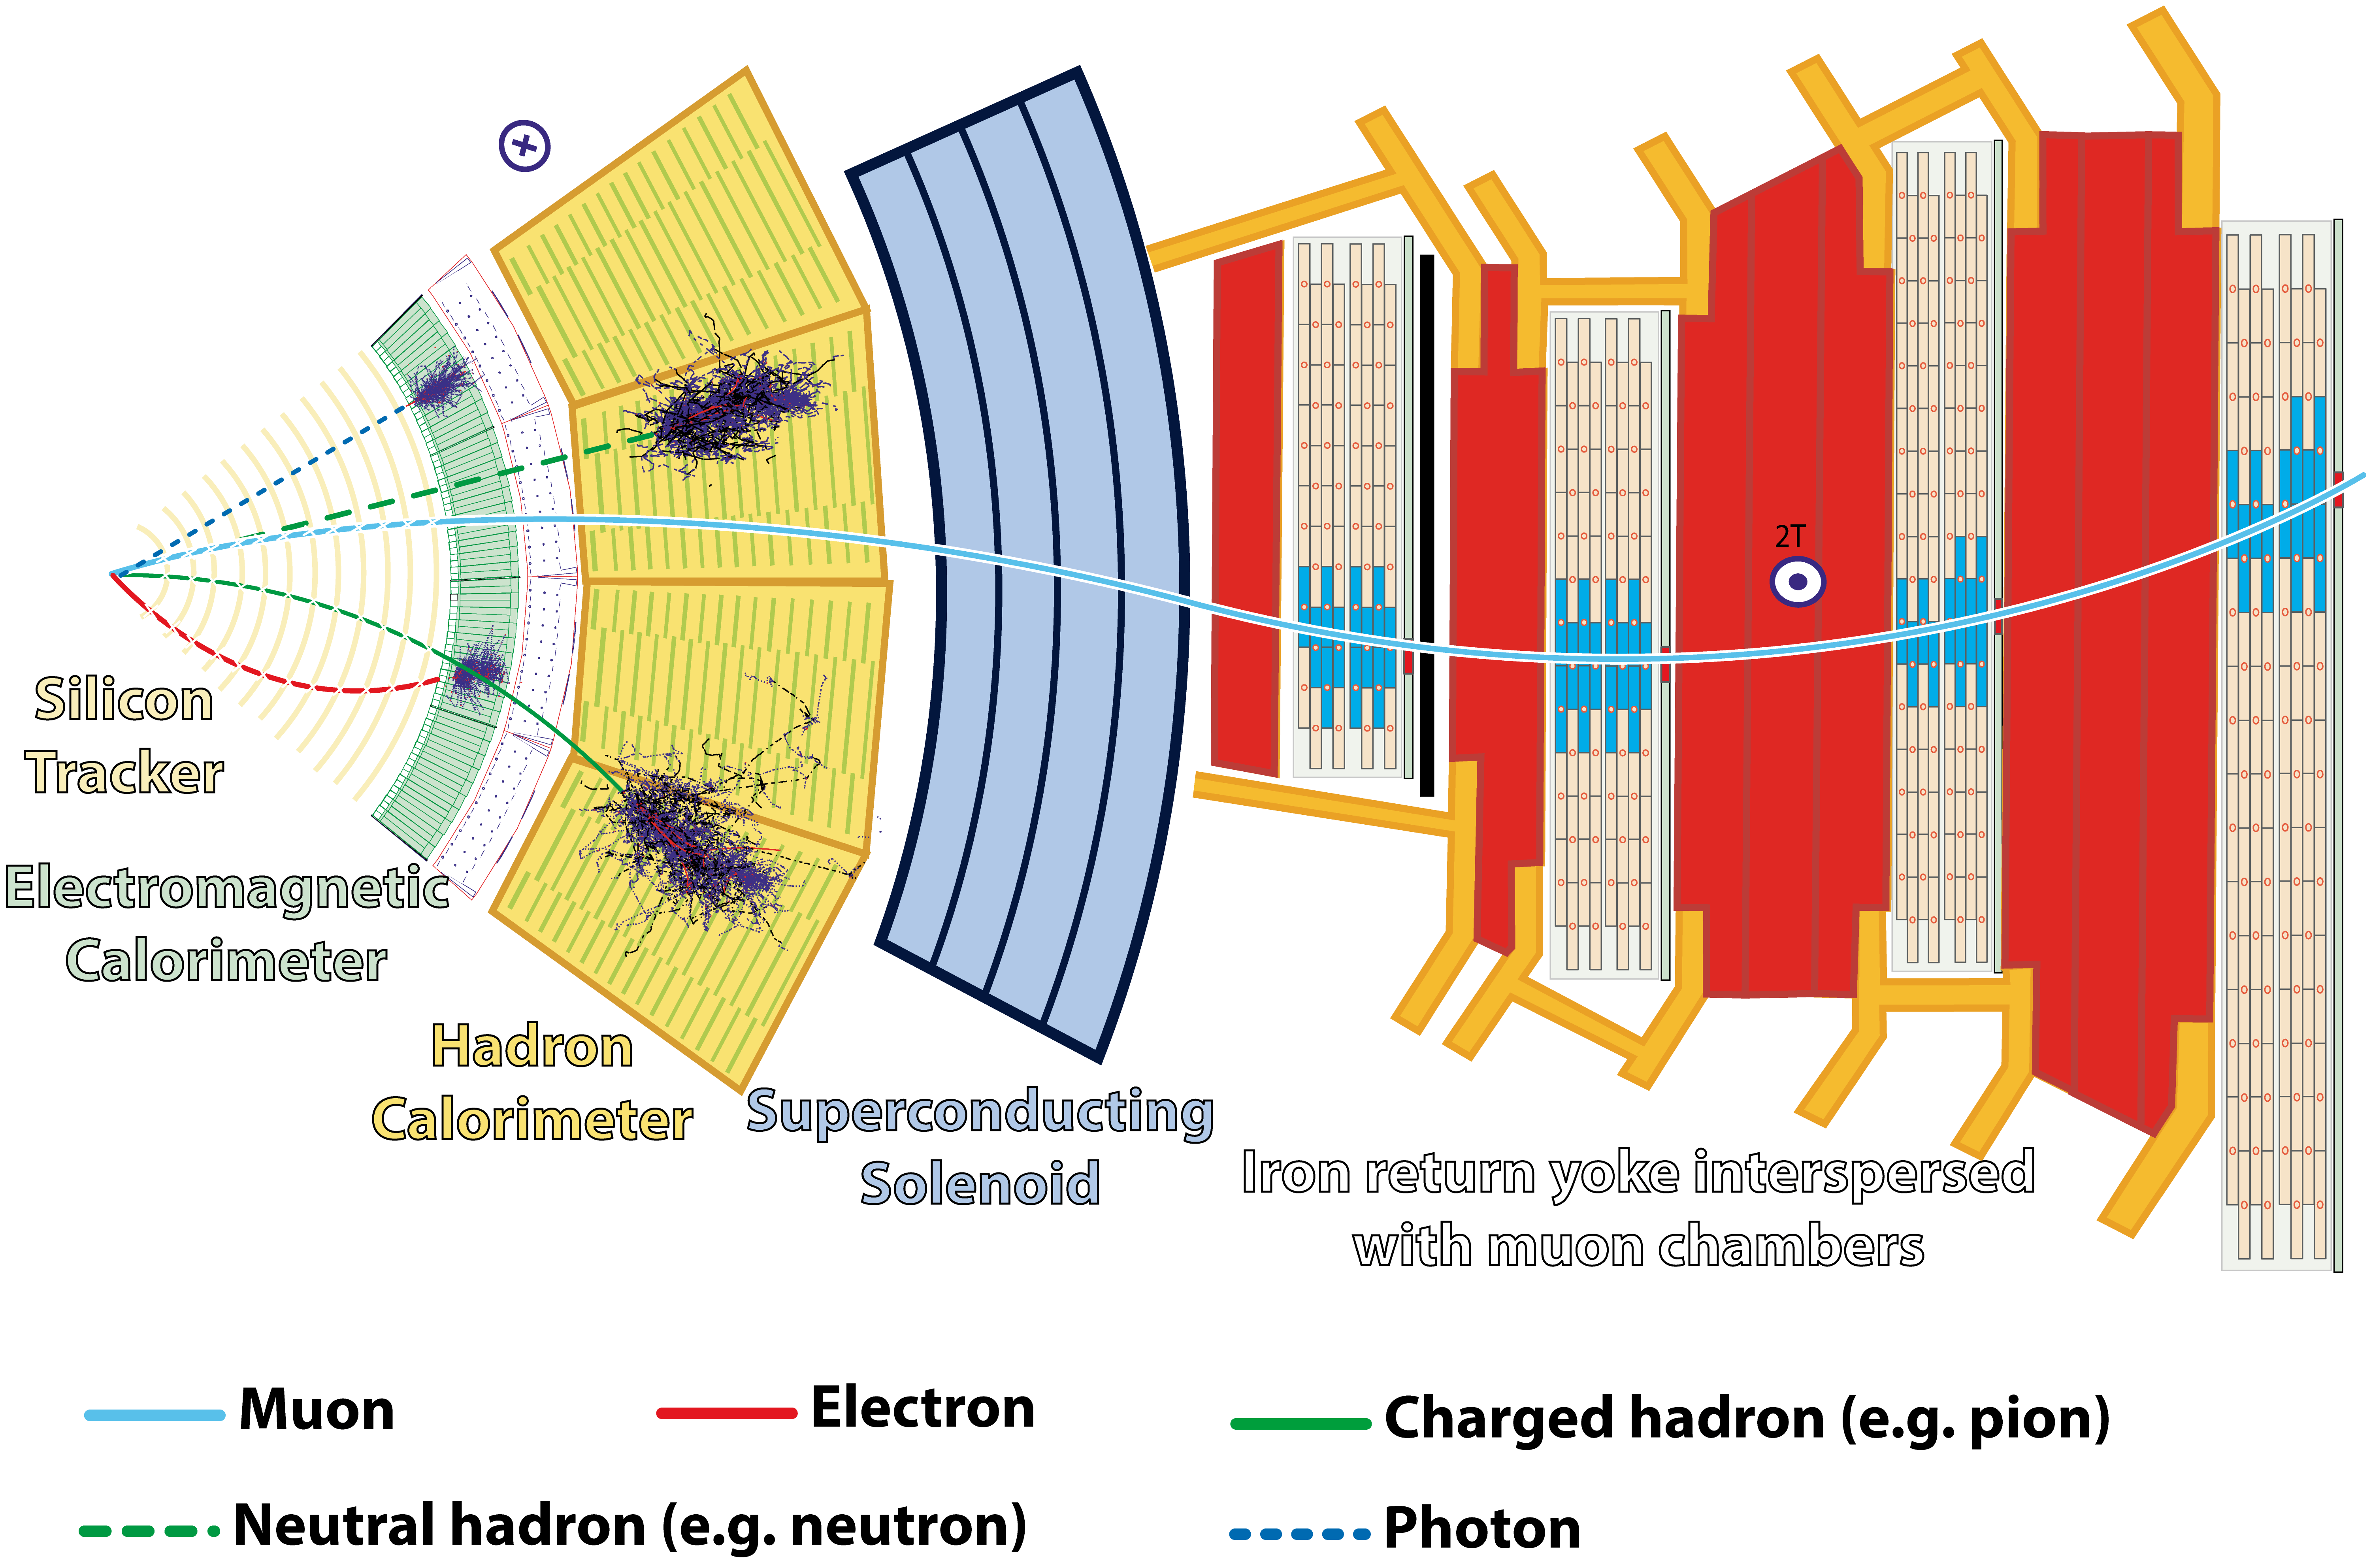
\includegraphics[width=.9\textwidth]{figs/cms/CMSslice_whiteBackground.png}
\caption{A slice of the CMS detector.\label{fig:CMSslice}}
\end{figure}


\section{Superconducting Solenoid}
\label{sec:magnet}
The central feature of the CMS detector is a
superconducting solenoid providing a uniform axial
magnetic field of 3.8\unit{T}  over a magnetic length of 12.5 \unit{m}
and a free-bore radius of 3.15 \unit{m}. The large bending power ($11.4$ \unit{T}\unit{m}) of the
superconducting magnet permits a precise measurement of the momentum
of high-energy charged particles. The return field is large enough to
saturate $1.5$ \unit{m} of iron, allowing four \emph{muon stations} to be
integrated.
% to ensure robustness and full geometric coverage.
The bore of the magnet coil is large enough to accommodate the inner tracker
and the calorimetry inside, thereby minimizing the amount of material
in front of the calorimeters.

\section{Silicon Tracker}
\label{sec:tracker}
The first layer of the detector encountered by outgoing particles from the
collisions is the tracker, composed of a small silicon pixel
surrounded by a large silicon strip tracker~\cite{Chatrchyan:2014fea}. Both tracker subdetectors are
cylinder-shaped and occupy a total $5.8$ \unit{m} in length and $2.5$
\unit{m} in diameter. The pixel detector barrel (endcaps) comprises three (two) layers of pixel
detectors, providing three-dimensional position measurements of the
hits arising from the interaction of charged particles with its
sensors. The hit position resolution is approximately $10$ $\mu$m in
the transverse coordinate and $20–40$ $\mu$m in the longitudinal
coordinate, while the third coordinate is given by the sensor plane
position. In total, its $1440$ modules cover an area of about 1
m$^{2}$ and have $66$ million pixels.

%The pixel detector consists of cylindrical barrel layers at radii of 4.4, 7.3 and 10.2 cm, and two pairs of endcap disks at z = ±34.5 and ±46.5 cm. It provides three-dimensional (3-D) position measurements of the hits arising from the interaction of charged particles with its sensors.

Surrounding this is the silicon strip tracker. The silicon detector
barrel (endcaps) has ten (twelve) layers of micro-strip detectors. In
total, the with
$15,148$ silicon modules, which cover an active area of about $198$
m$^2$ and have $9.3$ million strips. 

%It is composed of four subsystems. The Tracker Inner Barrel (TIB) and Disks
%(TID) cover r < 55 cm and |z| < 118 cm, and are composed of four
%barrel layers, supplemented by three disks at each end. These provide
%position measurements in rφ with a resolution of approximately 13–38
%μm. The Tracker Outer Barrel (TOB) covers r > 55 cm and |z| < 118 cm
%and consists of six barrel layers providing position measurements in
%rφ with a resolution of approximately 18–47 μm. The Tracker EndCaps
%(TEC) cover the region 124 < |z| < 282 cm. Each TEC is composed of
%nine disks, each containing up to seven concentric rings of silicon
%strip modules, yielding a range of resolutions similar to that of the
%TOB.

The fine granularity of the two tracker subdetectors offers separation of closely-spaced particle
trajectories in energetic jets. Fig.~\ref{fig:tracker} shows a
schemetic layout of the tracker in the $r-z$ plane and
the material budget of the CMS tracker, both in units of radiation
lengths and nuclear interaction lengths, as estimated from
simulation. 
%The simulation describes the tracker material budget with
%an accuracy better than 10\%, as was established by measuring the
%distribution of reconstructed nuclear interactions and photon
%conversions in the tracker.

\begin{figure}\centering
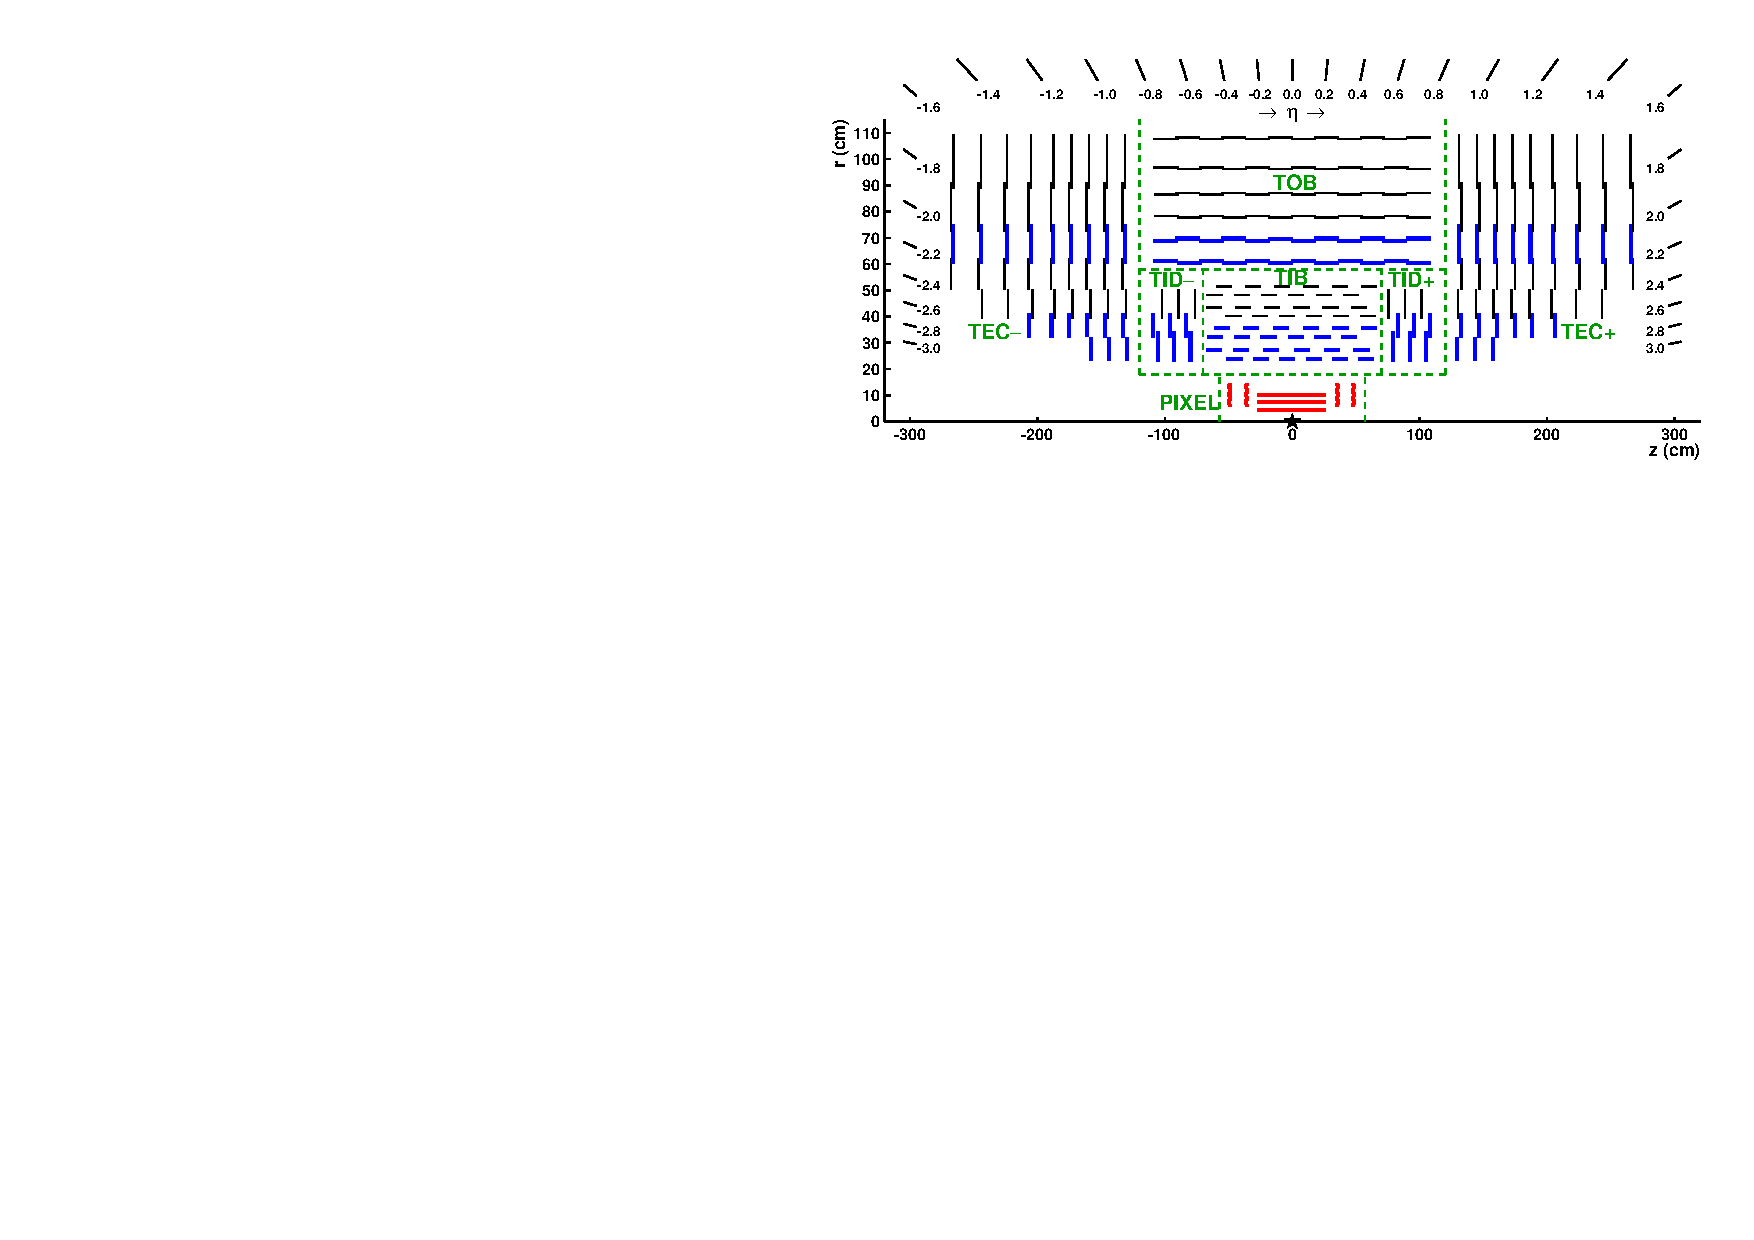
\includegraphics[width=.9\textwidth]{figs/cms/TrackerLayoutNew.pdf}\\
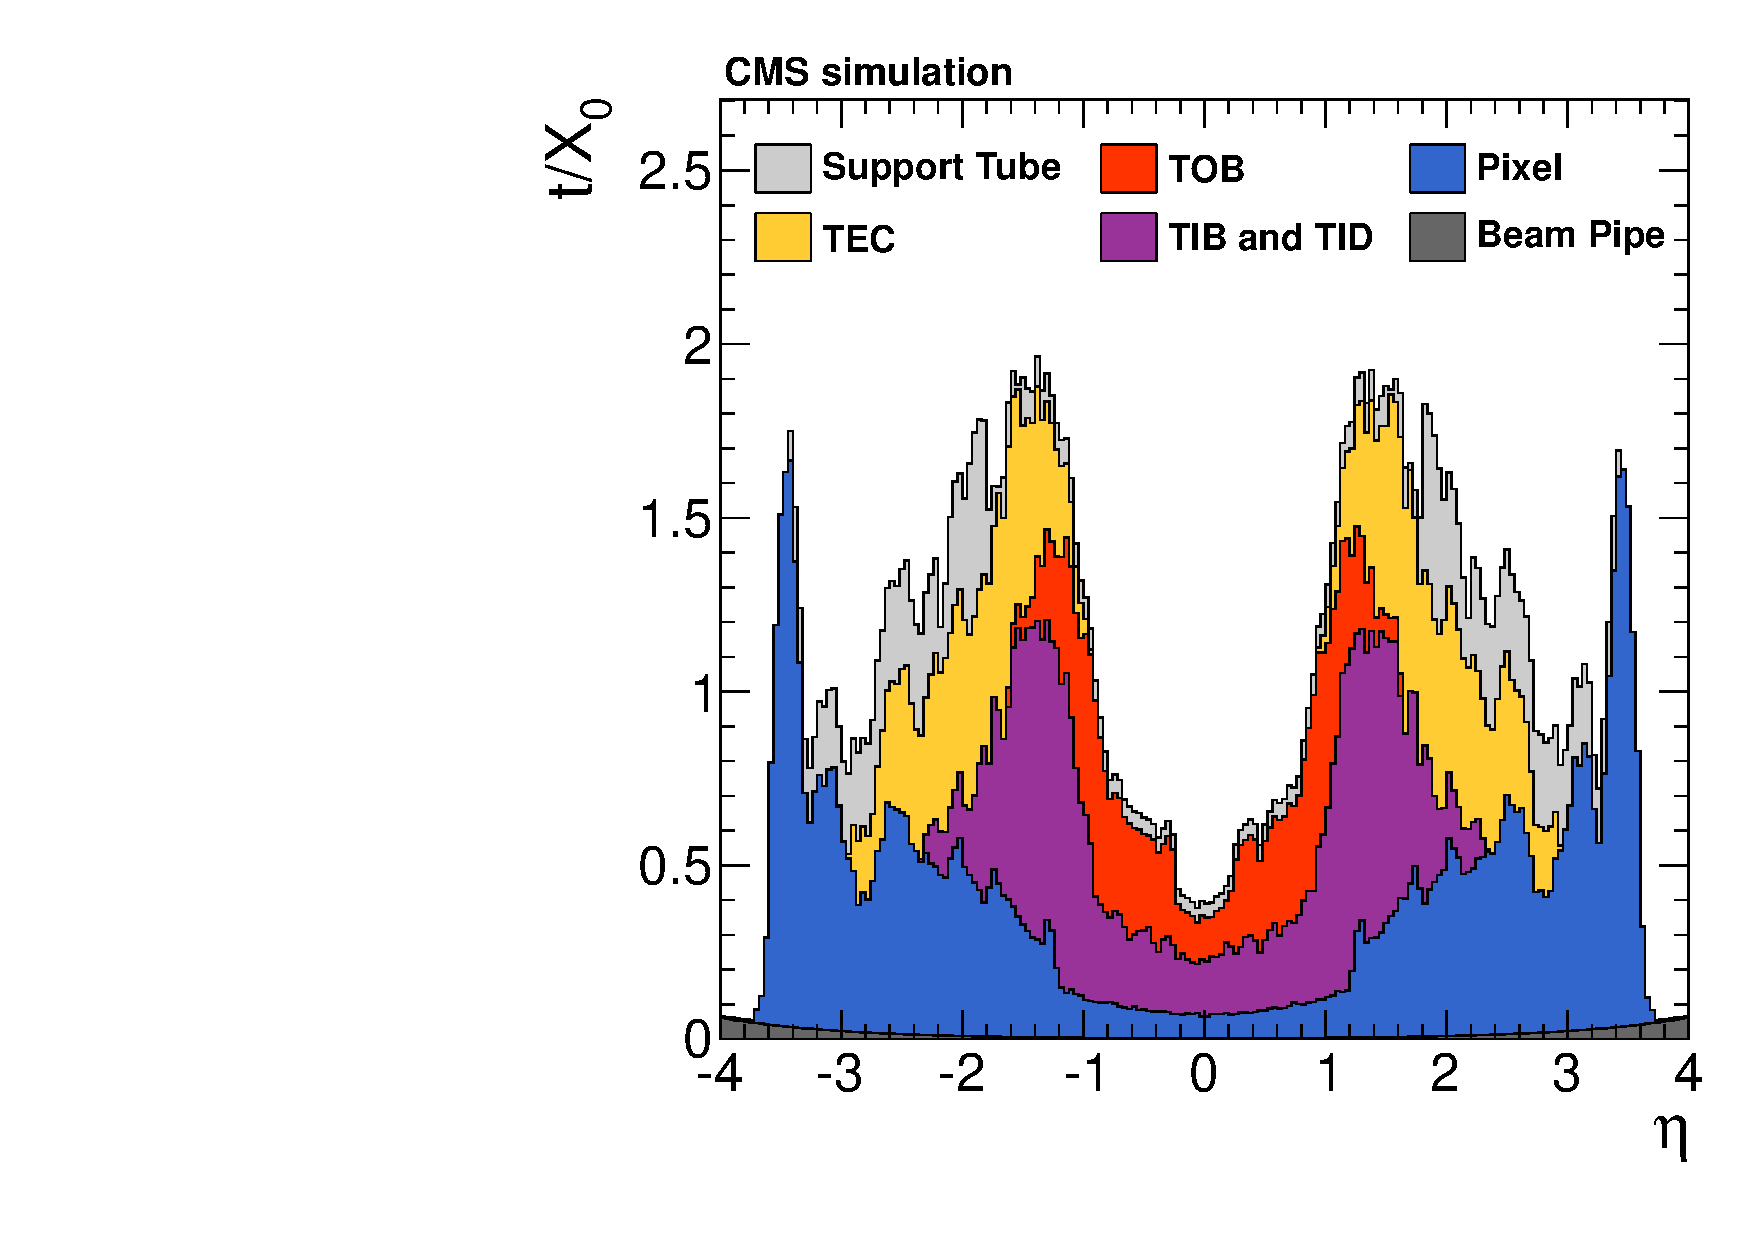
\includegraphics[width=.45\textwidth]{figs/cms/MaterialBudget_RadLengths.pdf}
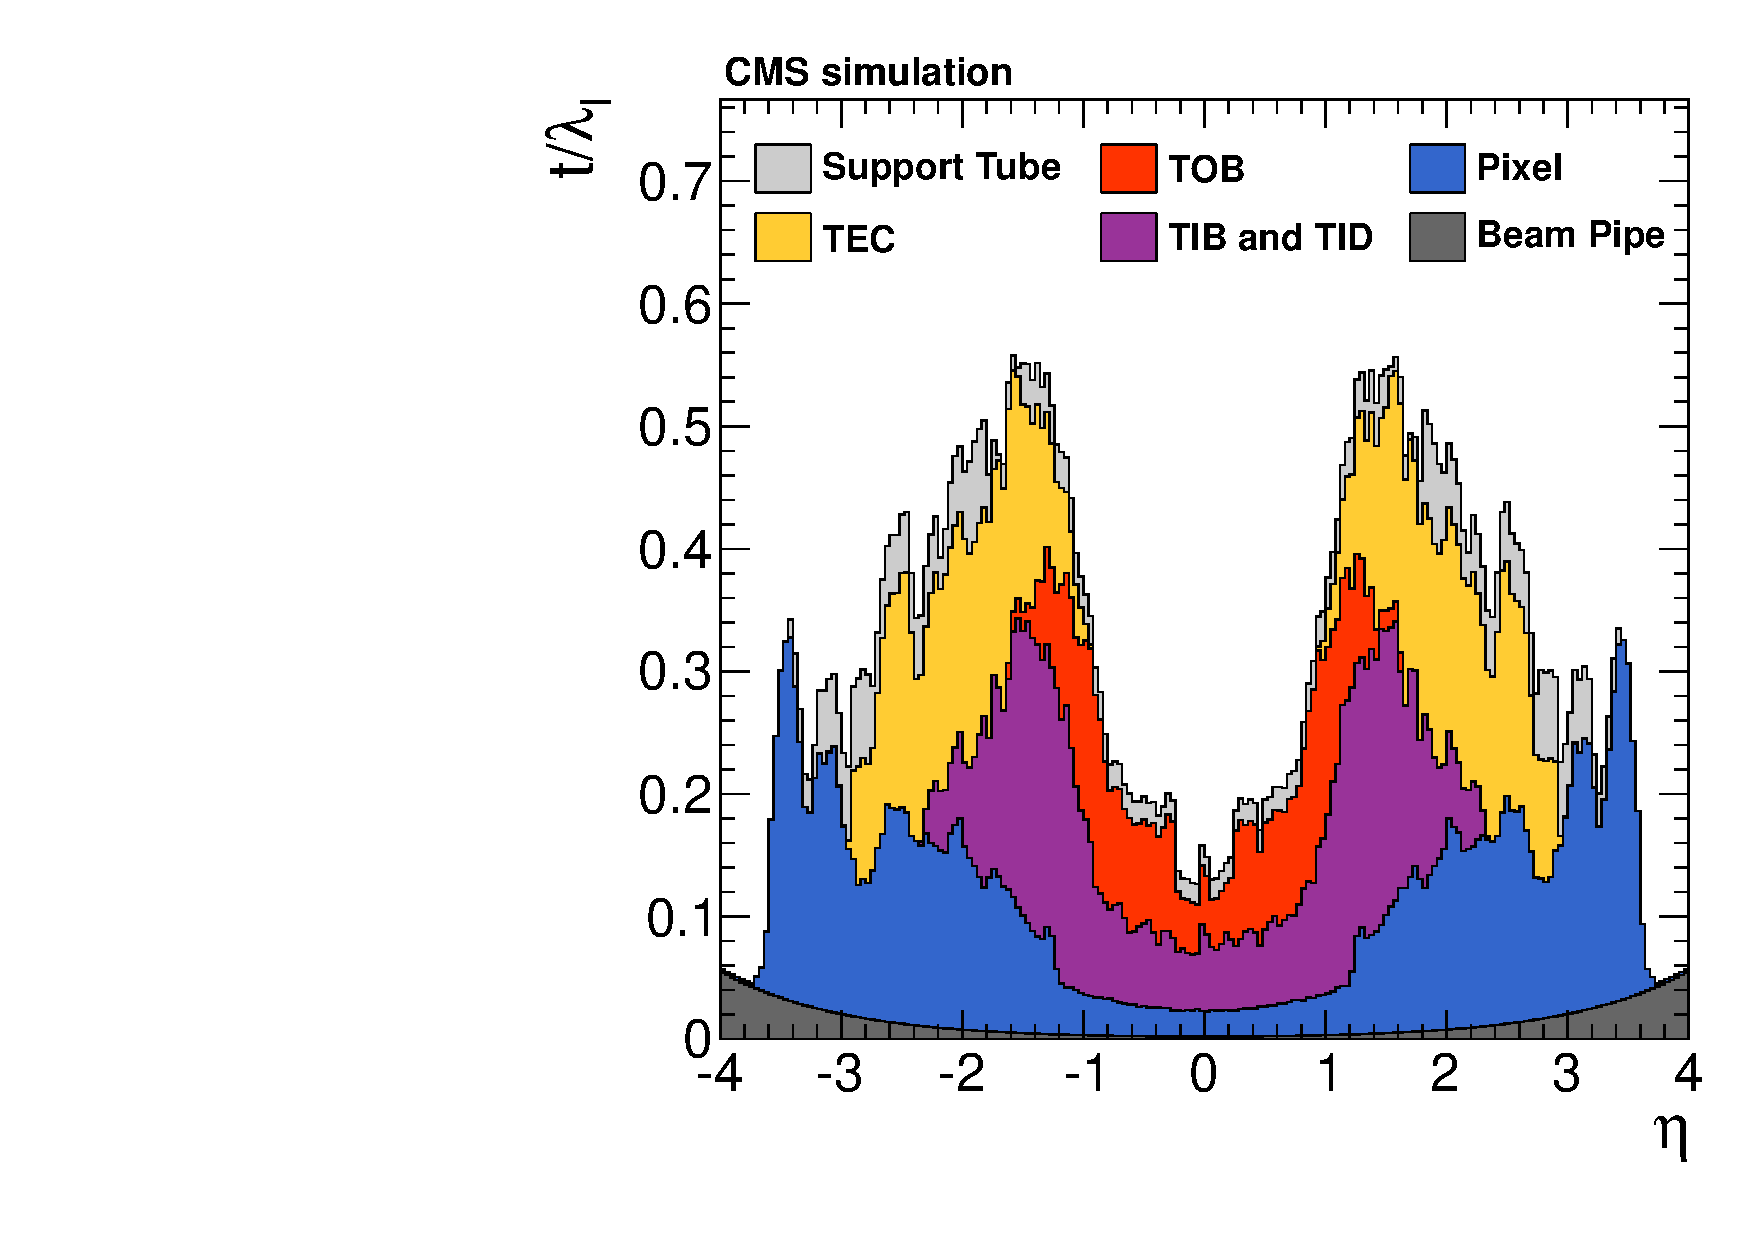
\includegraphics[width=.45\textwidth]{figs/cms/MaterialBudget_InteractionLengths.pdf}
\caption{(Top) Schematic cross section through the CMS tracker in the $r-z$
  plane. (Bottom) Total thickness $t$ of the tracker material
  traversed by a particle produced at the nominal interaction point,
  as a function of pseudorapidity $\eta$, expressed in units of radiation
  length $X_0$ (left) and nuclear interaction length $\lambda_I$
  (right). \label{fig:tracker}}
\end{figure}

%In this view, the tracker is symmetric about the horizontal
%  line $r = 0$, so only the top half is shown. The center of the
%  tracker, corresponding to the approximate position of the pp
%  collision point, is indicated by a star. Green dashed lines help the
%  reader understand which modules belong to each of the named tracker
%  subsystems. Strip tracker modules that provide 2D hits are shown by
%  thin, black lines, while those permitting the reconstruction of hit
%  positions in 3D are shown by thick, blue lines. The latter actually
%  each consist of two back-to-back strip modules, in which one module
%  is rotated through a `stereo' angle. The pixel modules, shown by the
%  red lines, also provide 3D hits. Within a given layer, each module
%  is shifted slightly in $r$ or $z$ with respect to its neighbouring
%  modules, which allows them to overlap, thereby avoiding gaps in the
%  acceptance.


\section{Electromagnetic Calorimeter}
\label{sec:ecal}

Within the superconducting solenoid volume and just outside of the
tracker, lies the electromagnetic calorimeter (ECAL) schematically
pictured in Fig.~\ref{fig:ecal}. The ECAL is a hermetic homogenous
calorimeter composed of 61,200 lead-tungstate (PbWO$_{4}$) scintillating crystals mounted in
the barrel covering $\abs{\eta}<1.479$, and 7,324 crystals mounted in the two endcap disks
covering $1.479<\abs{\eta}<3.0$. The high-density ($8.28$ g/cm$^{3}$),
short radiation length ($X_0 = 0.89$ cm), and small Moli\'{e}re radius
($R_M$ = 2.2 cm) of PbWO$_{4}$ allow the construction of a compact
calorimeter with fine granularity.

\begin{figure}
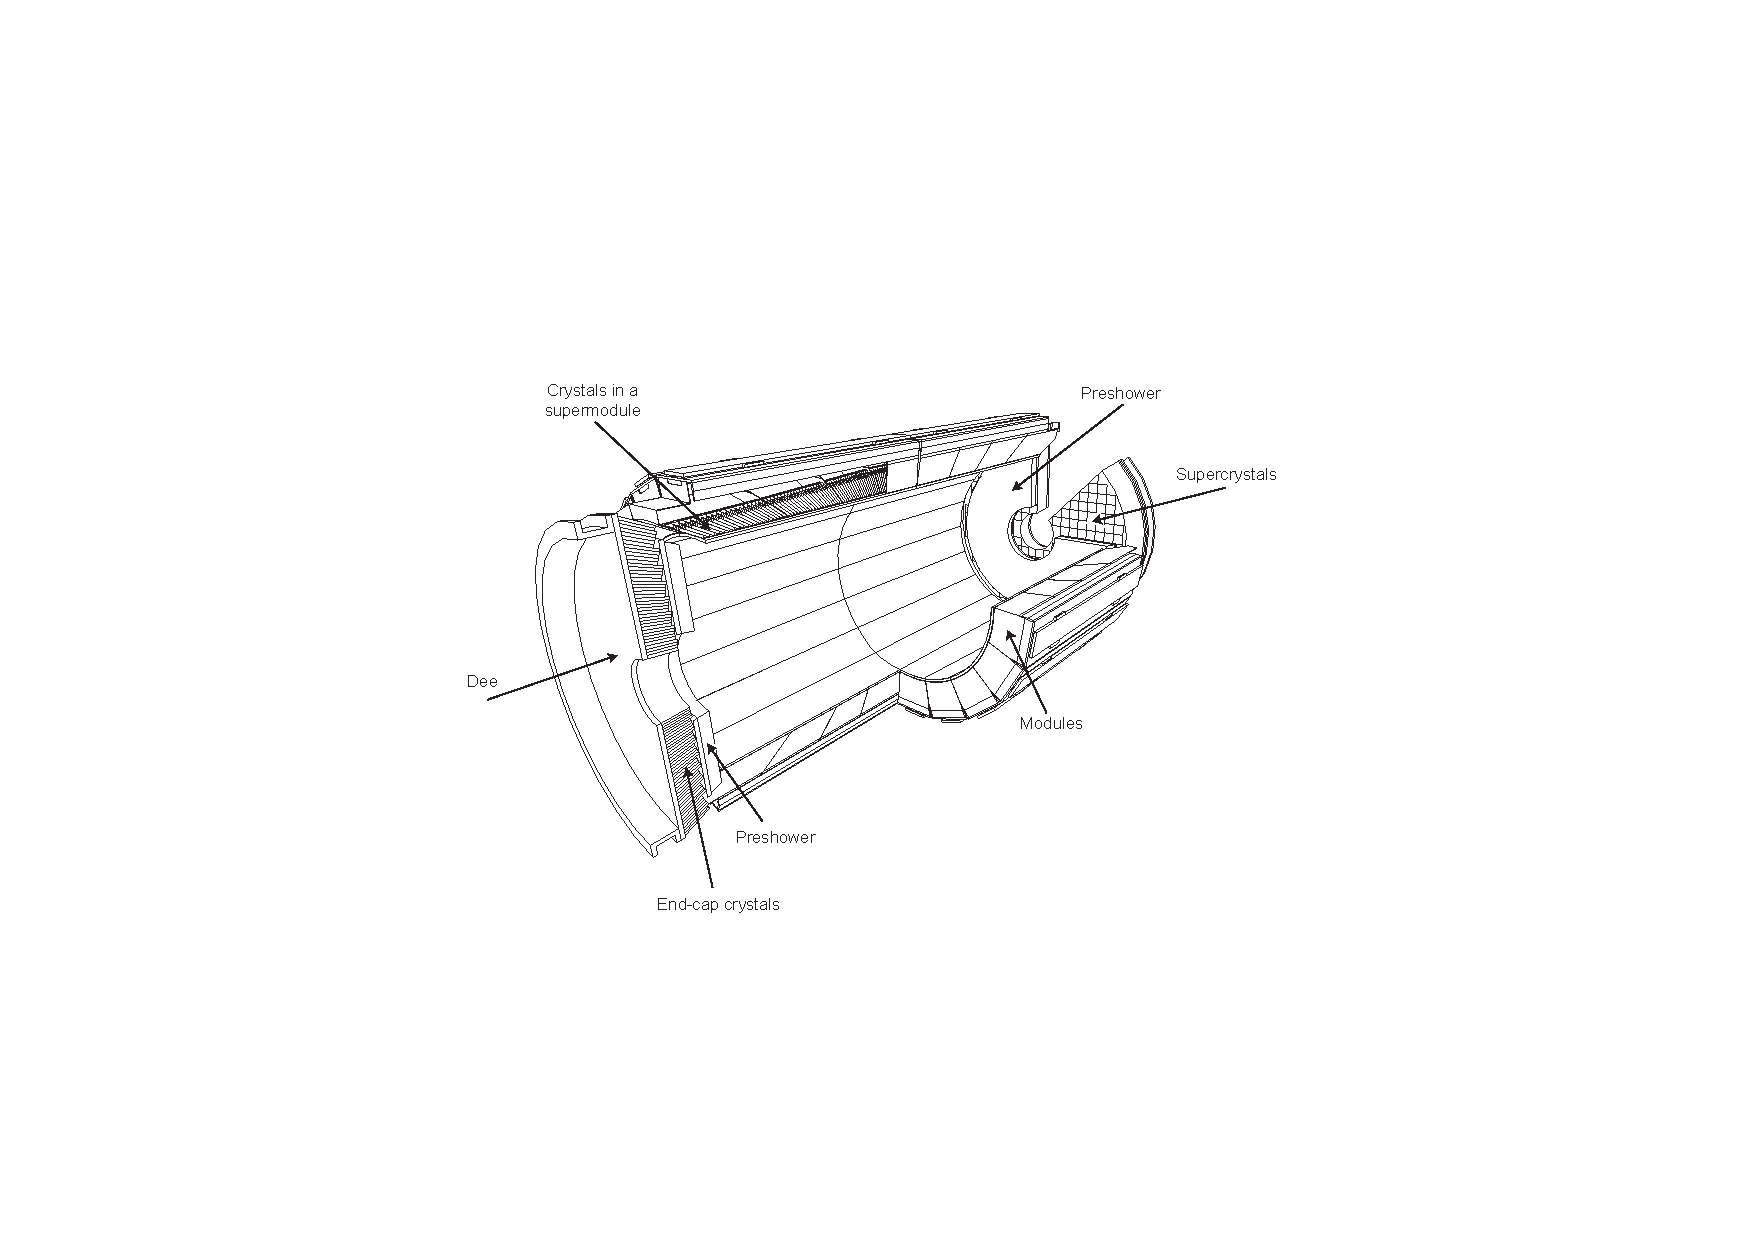
\includegraphics[width=.9\textwidth]{figs/cms/calorimeter.pdf}\centering
\caption{Layout of the CMS ECAL, showing the barrel supermodules, the
  two endcaps and the preshower detectors. The ECAL barrel coverage is
  up to $\abs{\eta} = 1.48$; the endcaps extend the coverage to $\abs{\eta} = 3.0$; the
  preshower detector fiducial area is approximately $1.65 < \abs{\eta}
  < 2.6$.\label{fig:ecal}}
\end{figure}

The crystal length of $23$ ($22$) \unit{cm}, corresponding to $25.8$
($24.7$) radiation lengths in the barrel (endcaps), is sufficient to
contain more than 98\% of the energy of electrons and photons up to
$1$ \TeV. The crystal material also amounts to about one nuclear interaction
length, causing about two thirds of the hadrons to start showering in
the ECAL.

The barrel crystal front face has an area of  $2.2 \times 2.2$ cm$^2$, equivalent to $0.0174 \times 0.0174$ in the ($\eta,\phi$)
plane, while in the endcaps, the crystals are arranged instead in a
rectangular ($x, y$) grid, with a front-face area of $2.9 \times 2.9$
cm$^{2}$. The crystal transverse size in the barrel matches the small Moli\`{e}re radius of
PbWO$_4$ ($2.2$ cm). This fine transverse granularity makes it possible to fully resolve hadron and photon
energy deposits as close as $5$ \unit{cm}. 
% for the benefit of exclusive particle identification in jets up to
% very large transverse momentum. 

The PbWO$_4$ crystals emit blue-green scintillation light with a broad
maximum at wavelengths $420–430$ \unit{nm}. The quantum efficiency and surface
coverage of the photodetectors are such that a particle depositing $1$
\unit{MeV} of energy in a crystal produces an average signal of about
$4.5$ photoelectrons.
% The stability of the temperature
%and of the photodetector gain are critical for an accurate
%determination of the energy deposited in the crystals.

The ECAL barrel energy resolution for electrons is measured in
an electron test beam to be~\cite{Adzic:2007mi,Chatrchyan:2013dga},
\begin{align}
\frac{\sigma_E}{E} &= \frac{S}{\sqrt E (\GeV)} \oplus \frac{N}{E (\GeV)} \oplus C \\
&= \frac{2.8\%}{\sqrt E (\GeV)} \oplus \frac{12\%}{E (\GeV)} \oplus 0.3\%
\end{align}
%\\&= \frac{7\%}{\sqrt E (\GeV)} \oplus \frac{35\%}{E (\GeV)} \oplus 0.7\%
where the three contributions are the stochastic, noise, and constant
terms.

A finer-grained detector, known as the preshower, is installed in
front of each endcap disks. It consists of two layers, each comprising
a lead radiator followed by a plane of silicon strip sensors, with a
pitch of $1.9$ \unit{mm}. The goal of the preshower is to enhance photon
identification capabilities.

Since ECAL crystals are approximately one Moli\'ere radius in lateral
dimension, high energy electromagnetic showers spread laterally over
several crystals. 
%Furthermore, in CMS, the presence of material in
%front of the electromagnetic calorimeter (corresponding to 1--2$\,X_0$
%depending on the $\eta$ region) causes conversion of photons and
%bremsstrahlung from electrons. The strong magnetic field of the
%experiment tends to spread this radiated energy along $\phi$.
Clustering algorithms are used to sum together energy
deposits in adjacent crystals belonging to the same electromagnetic
shower. The clustering algorithm proceeds first with the formation of ``basic clusters'', corresponding
to local maxima of energy deposits. The basic clusters are then merged
together to form a ``supercluster'', which is extended in
$\phi$, to recover the radiated energy. Because of the differences
between the geometric arrangement of the crystals in the barrel and
endcap regions, a different clustering algorithm is used in each
region. The clustering algorithm used in EB, called the `hybrid'
algorithm, is described in~\cite{CMS_TDR_v1}. In EE and ES, the
algorithm merges together fixed-size 5$\times$5 crystal basic clusters
and associates each with corresponding ES energy deposits.

\section{Hadron Calorimeter}
\label{sec:hcal}

The ECAL is surrounded by a hermetic sampling hadron
calorimeter (HCAL) consisting of several layers of brass absorber and plastic scintillator
tiles interleaved. A barrel detector ($\abs{\eta}<1.3$) and two endcap
disks ($1.3<\abs{\eta}<3.0$) provide pseudorapidity coverage up to
$3.0$. The scintillation light is converted by wavelength-shifting (WLS) fibers
embedded in the scintillator tiles and channeled to photodetectors via
clear fibers. This light is detected by photodetectors (hybrid
photodiodes, or HPDs) that can provide gain and operate in high axial
magnetic fields. This central calorimetry is complemented by a
tail-catcher in the barrel region (HO) ensuring that hadronic
showers are sampled with nearly 11 hadronic interaction
lengths.

The HCAL is read out in individual towers with a cross section of
$\Delta\eta\times\Delta\phi = 0.087 \times 0.087$ for $\abs{\eta}<1.6$
and $0.17\times 0.17$ at larger pseudorapidities. The HCAL energy resolution is measured in a pion test beam to
be~\cite{Abdullin:2009zz}
\begin{align}
\frac{\sigma_E}{E} &= \frac{110\%}{\sqrt E (\GeV)} \oplus 9\%~.
\end{align}

Coverage up to a pseudorapidity of $5.0$ is provided by a forward
hadron calorimeter (HF) situated at $11$ \unit{m} from the interaction
point.The HF consists of a steel absorber composed of grooved
plates. Radiation-hard quartz fibers are inserted in the grooves along
the beam direction. The signals from the fibers are grouped
so as to define calorimeter towers with a cross section of $\Delta\eta\times\Delta\phi = 0.175 \times
0.175$ over most of the pseudorapidity range. The \v{C}erenkov light emitted in the
quartz fibers is detected by photomultipliers. The forward
calorimeters ensure full geometric coverage, which is especially
important for the measurement of the
transverse energy in the event.

\section{Muon System}
\label{sec:muon}

The most outward part of the CMS detector is the muon spectrometer,
made up of four stations of gas-ionization detectors sandwiched between
three layers of iron return yoke. Drift tube (DT) chambers and cathode strip chambers (CSC) detect muons
in the regions $\abs{\eta} < 1.2$ and $0.9 < \abs{\eta} < 2.4$,
respectively, and are complemented by a system of resistive plate
chambers (RPC) covering the range $\abs{\eta} < 1.6$.  The
reconstruction involves a global trajectory fit across the muon
stations and the inner tracker. Due to the large amount of material before the muon chambers, low-\pt muons
undergo multiple scattering and thus the inner tracker dominates the
momentum measurement up to a muon \pt of about $300$ \GeV.

\section{Particle-Flow Reconstruction}
\label{sec:pf}
%The versatile, albeit simple, design of the CMS apparatus features
%most of the proper- ties required for particle-flow reconstruction: a
%granular tracker, a fine-grained elec- tromagnetic calorimeter, a
%hermetic hadron calorimeter, a large magnetic field, and an accurate
%muon spectrometer. 

Each particle yields a specific signature in the CMS detector: compared to charged
hadrons, electrons have no HCAL cluster; neutral hadrons have no
tracks; photons have neither of those; and muons leave a signal in the
muon chambers. Traditional reconstruction methods typically utilize
the information from only one subdetector in reconstrucing a
particular physics object: for example, jets are traditionally
reconstructed using only information from the HCAL. 

%Establishing a connection between the information
%provided by the successive detector layers provides a
%greater level of robustness to particle identifciation and determination of the particle
%properties.
%Thanks to the fine spatial granularity of the
%CMS detector, the final-state particles arising from
%LHC proton-proton collisions can be individually identified and
%reconstructed with an optimal combination of the information from
%all sub-detectors. 
The \emph{particle-flow (PF) reconstruction algorithm}, developed before the start of the
LHC, commissioned with the first 2010 data at
$\sqrt{s}=7$ \TeV, and still in use during Run 2, is an attempt to
construct a global event description based on an optimal combination
of information from all subdetectors. Individual particles (PF candidates) are reconstructed by combining the information from the inner
tracker, the calorimeters, and the muon system. Five categories of PF
candidates are defined: muons, electrons, photons (including their
conversions to $\Pep\Pem$ pairs), charged hadrons, and neutral
hadrons. This global event description leads to significantly improved performance for electron and muon identification, jet and
hadronic $\tau$ decay reconstruction, and missing transverse energy
evaluation. 

This approach enables the mitigation of effects due to
particles produced by additional $\Pp\Pp$ collisions in the same or in neigboring bunch
crossings (pileup). Charged PF candidates not compatible
with the interaction point are discarded and when computing lepton
isolation and jet energy, the corresponding contamination from neutral
particles is subtracted on average by applying an event-by-event correction based on the jet-area
method~\cite{jetarea_fastjet,jetarea_fastjet_pu,JME-JINST}. PF reconstruction also minimizes the need
for a posteriori corrections inherent to the information missing in
the traditional physics object reconstruction path. 

\subsection{Jets and Missing Transverse Energy}

To demonstrate the effectiveness of PF reconstruction over traditional
calorimeter-based (Calo) reconstruction, we can examine the response
and resolution of jets and missing transverse energy, the most
important physics objects in the searches for SUSY outlined in
Ch.~\ref{ch:analysis8TeV} and Ch.~\ref{ch:analysis13TeV}, with both
methods of reconstruction.

Jets are reconstructed with the anti-$\kt$ algorithm
\cite{antikt,fastjet} and a distance parameter $R=0.4$, clustering either the particles reconstructed by the
particle-flow algorithm (PF jets), the energy deposits observed in the
calorimeters (Calo jets), or the stable particles produced by the
event generator (Ref jets).

Each PF (Calo) jet is matched to the closest Ref jet within a cone of
angle 0.1 (0.2) in the $(\eta, \phi)$ space. The use of a twice
smaller cone angle for PF jets is justified by a twice better
resolution on the measurement of the jet direction, shown in
Fig.~\ref{fig:expected_performance_jets_angular}. 
The improved angular resolution for PF jets is mainly due
to the precise determination of the charged-hadron direction and
momentum. In Calo jets, the energy deposits of charged hadrons are spread
along the $\phi$ direction by the magnetic field, leading to a
degraded azimuthal resolution. 

\begin{figure}[htb]\centering 
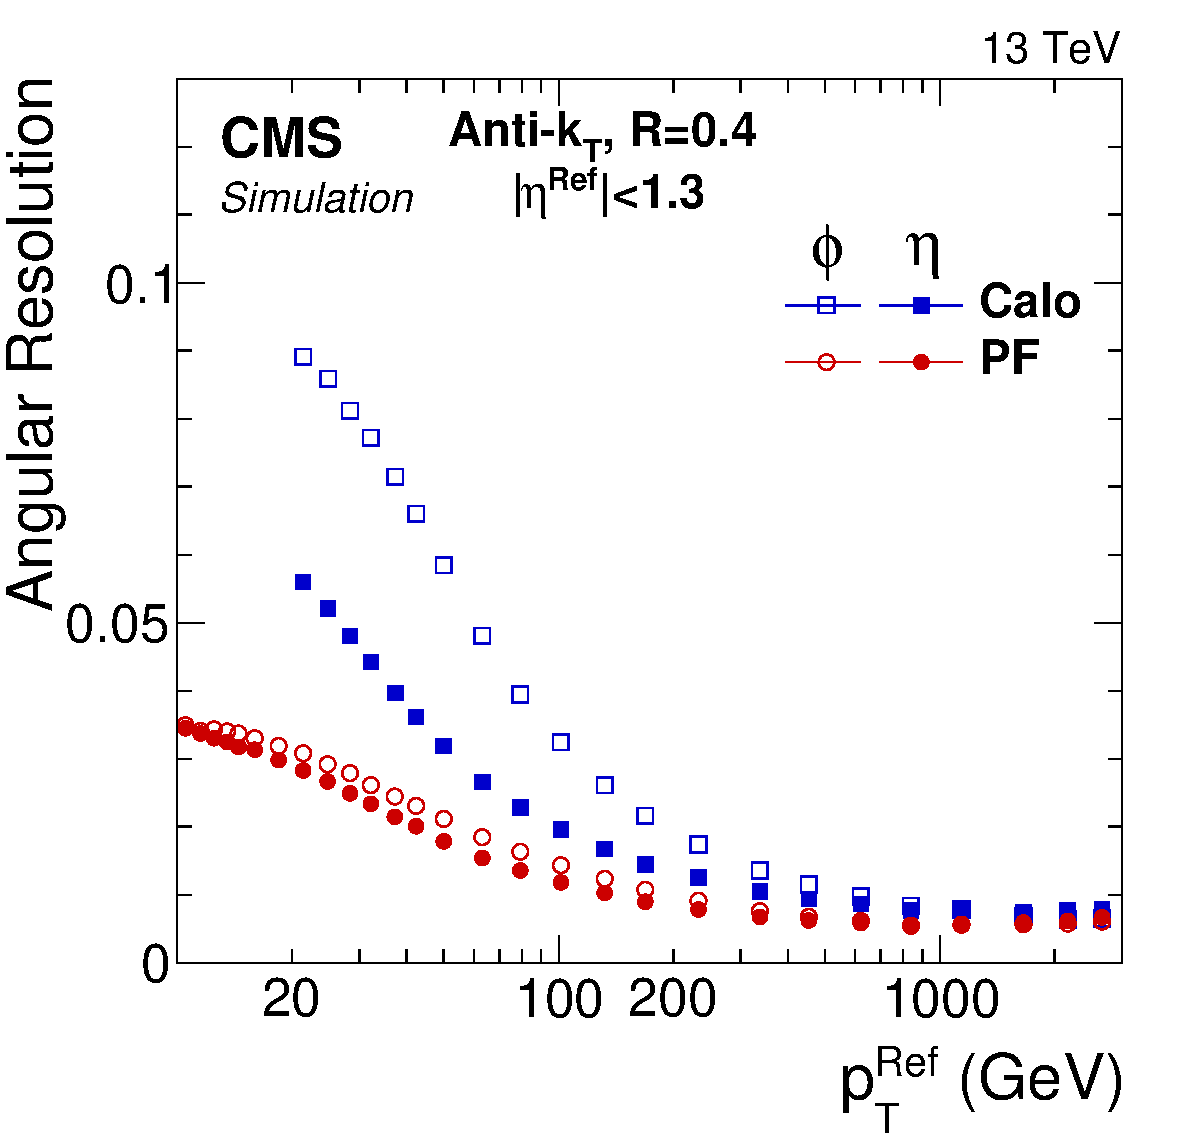
\includegraphics[width=0.45\textwidth]{figs/cms/EtaPhiResVsRefPt_Barrel_AK4CaloL2L3_AK4PFL2L3_RMS_no2000.pdf} 
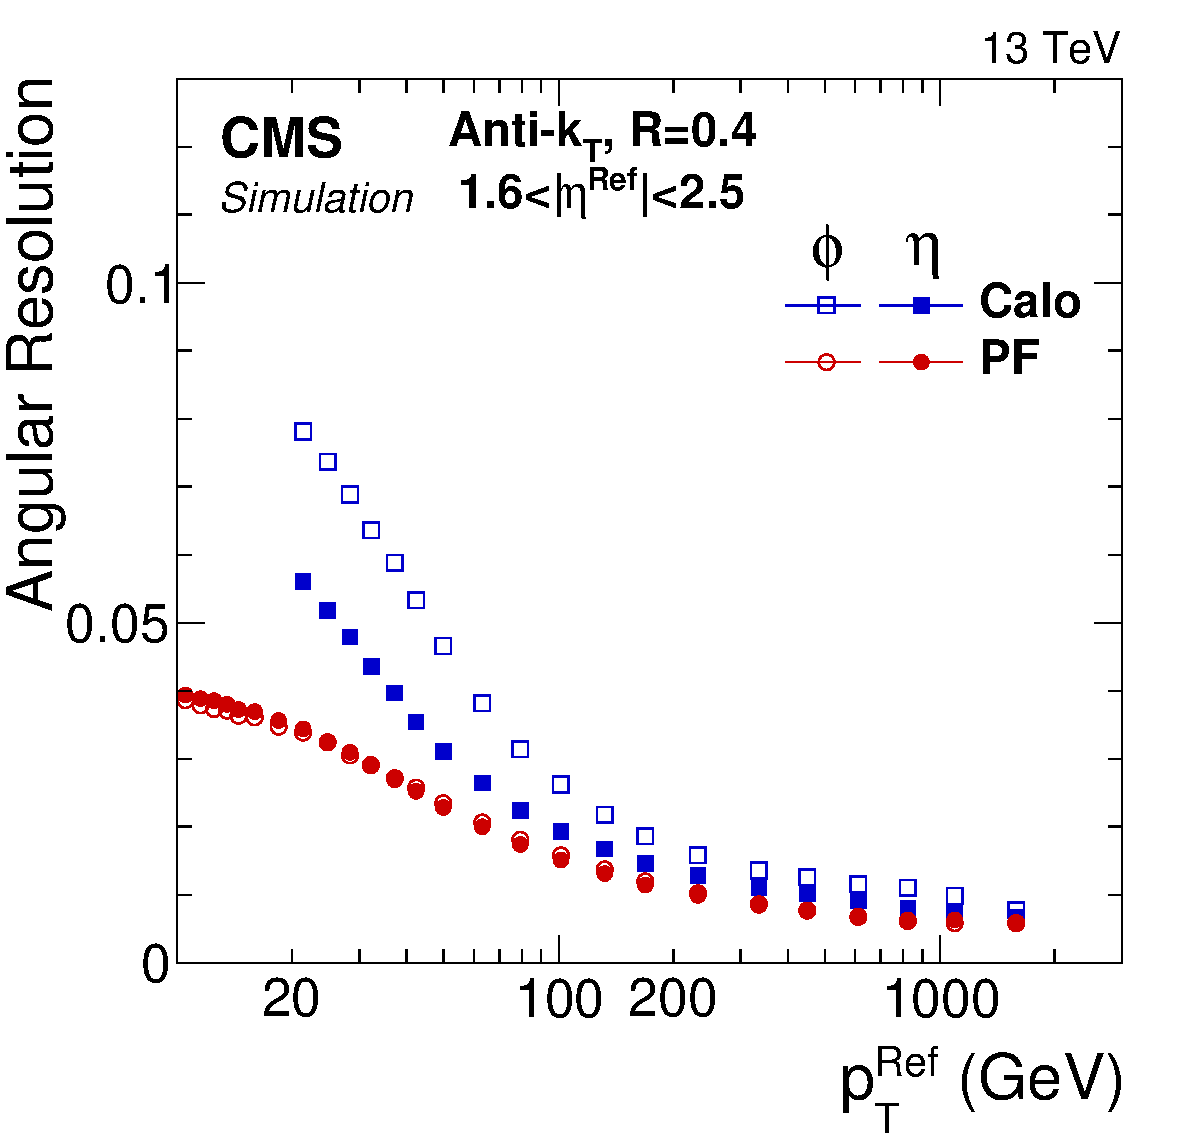
\includegraphics[width=0.45\textwidth]{figs/cms/EtaPhiResVsRefPt_Endcap_AK4CaloL2L3_AK4PFL2L3_RMS_no2000.pdf}
\caption{Jet angular resolution in the barrel (left) and endcap (right) regions, as a function of the transverse momentum of the reference jet.\label{fig:expected_performance_jets_angular}}
\end{figure}


%On average, 65\% of the jet energy is carried by charged hadrons, 25\%
%by photons, and 10\% by neutral hadrons. The ability of the PF
%algorithm to identify these particles in the jets is studied by
%comparing the jet energy fractions measured by the particle flow to
%the ones of the corresponding Ref jet. A significant portion of the
%transverse momentum carried by neutral hadrons is reconstructed as
%photons because the energy deposits of neutral hadrons in the ECAL are
%systematically used to reconstruct photons. Summing up the
%reconstructed energy from photons and neutral hadrons, around 80\% of the neutral hadron energy
%is recovered.

The raw jet energy response, defined as the mean ratio of the
reconstructed jet energy to the reference jet energy, is shown in
Fig.~\ref{fig:expected_performance_jets}. The PF jet response is
linear as a function of the jet transverse momentum and is above 90\%
across the whole detector acceptance. A jet energy correction procedure is used to bring the jet energy
response to unity, removing any dependence on \pt and
$\eta$~\cite{Khachatryan:2016kdb}. After this correction, the jet
energy resolution, defined as the Gaussian width of the ratio between
the corrected and reference jet energies, is also shown in Fig.~\ref{fig:expected_performance_jets}.

\begin{figure}[htbp]
  \centering 
  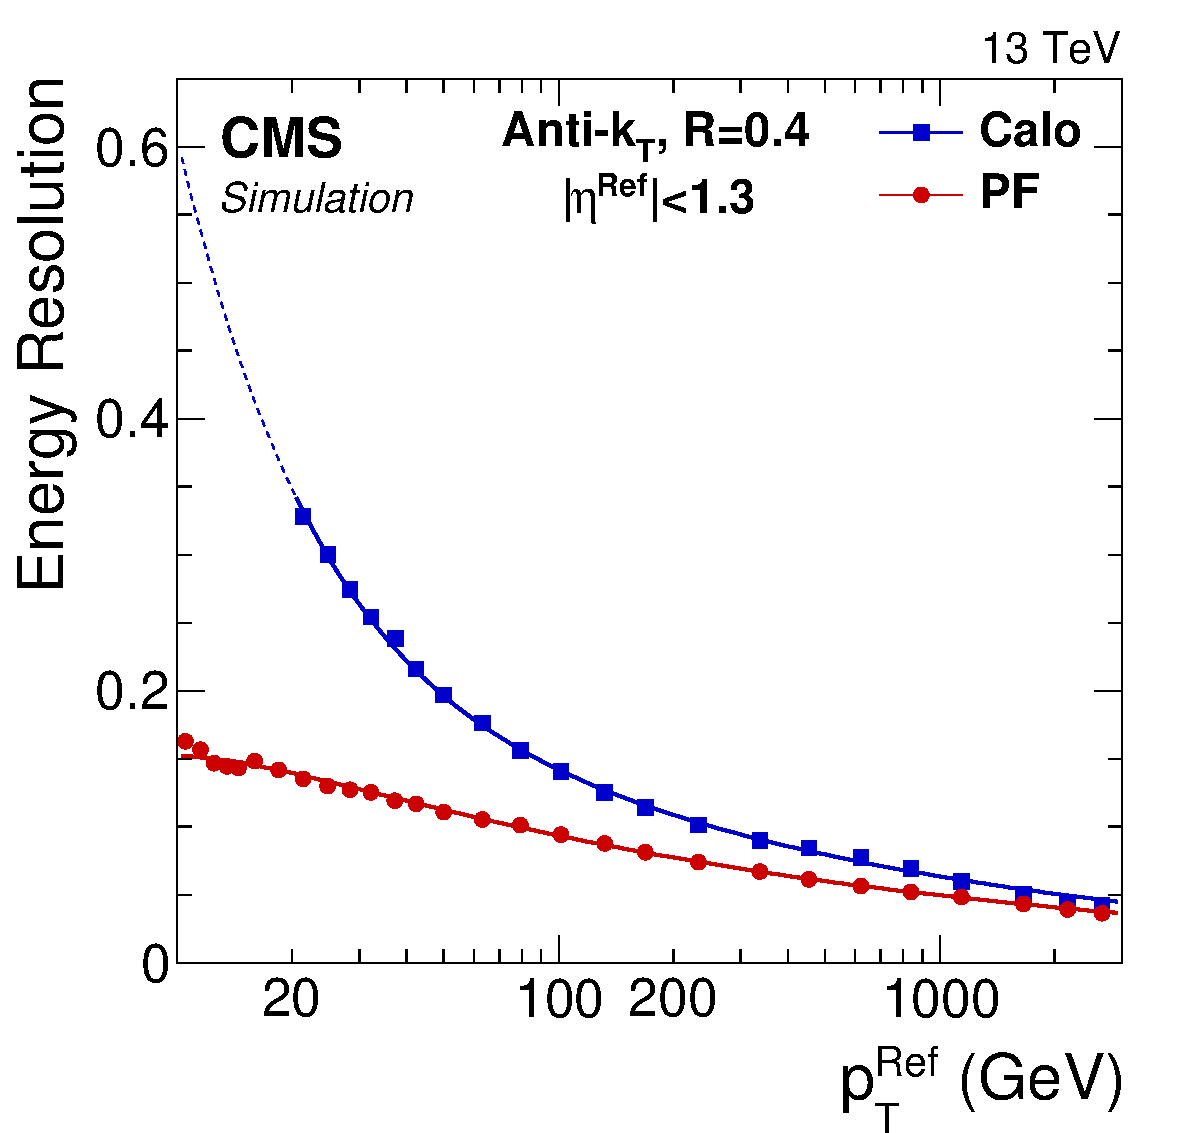
\includegraphics[width=0.45\textwidth]{figs/cms/RelResVsRefPt_Barrel_AK4CaloL2L3_AK4PFL2L3_no2000.pdf}
  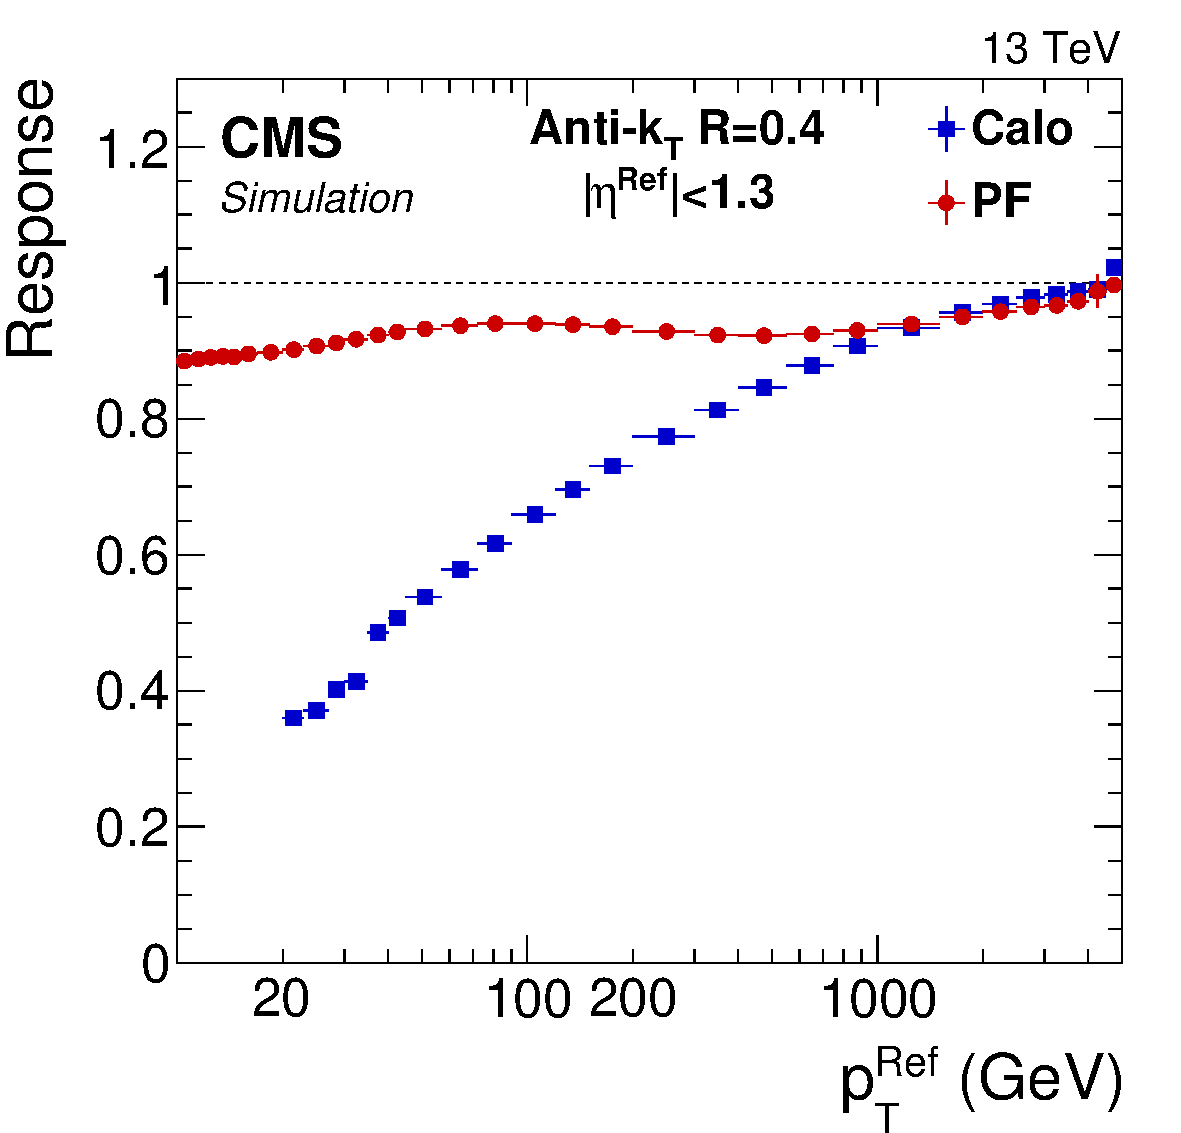
\includegraphics[width=0.45\textwidth]{figs/cms/ClosureRatioVsRefPt_RefEta0to1dot3_ak4caloOverak4pf_no2000.pdf}
  \caption{Jet \pt resolution (left) and jet \pt response (right) as a function of $\pt^{\mathrm{Ref}}$ in the barrel.\label{fig:expected_performance_jets}}
\end{figure}

The presence of particles that do not interact with the detector
material, such as a hypothetical dark matter particle, or simply
neutrinos, is indirectly revealed by missing transverse momentum,
often referred to as missing transverse energy~\cite{Khachatryan:2014gga}. The raw missing transverse momentum
vector is defined in such a way as to balance the vectorial sum of the
transverse momenta of all particles,
\begin{equation}
  \vecptmiss ({\mathrm{PF, raw}}) = - \sum_{i=1}^{N_{\mathrm{particles}}} \vecpt^{\,i}.
\end{equation}
The jet-energy-corrected missing transverse momentum,
\begin{equation}
  \vecptmiss ({\mathrm{PF}}) = - \sum_{i=1}^{N_{\mathrm{particles}}}
  \vecpt^{\,i} - \sum_{j=1}^{N_{\mathrm{PF\,jets}}} ({\vec p^{\,\mathrm{corr}\,j}_{\mathrm T}} - \vecpt^{\,j})~,
\end{equation}
includes a jet energy correction term that replaces the raw momentum
$\vecpt^{\,j}$  of each PF jet with $\vecpt^{\,j} >10\,\GeV$ by its
corrected value $\vec p^{\,\mathrm{corr}\,j}_{{\mathrm T}}$.
As seen in Fig.~\ref{fig:expected_performance_jets}, the
PF jet response is close to unity, making this correction term small
when the missing transverse energy is evaluated with reconstructed
particles.

Before the advent of PF reconstruction, the missing transverse
momentum was evaluated using information from the calorimeters and the
muon system as,
\begin{equation}
  \vecptmiss ({\mathrm{Calo}}) = - \sum_{i=1}^{N_{\mathrm{cells}}}
  \vecpt^{\,i} - \sum_{j=1}^{N_{\mathrm{Calo\,jets}}} ({\vec p^{\,\mathrm{corr}\,j}_{\mathrm T}} - \vecpt^{\,j}) - \sum_{k=1}^{N_{\mathrm{muons}}} \vecpt^{\,k}~,
\end{equation}
where in the first term, the transverse momentum $\vecpt^{\,i}$ of a
given calorimeter cell is calculated assuming that the energy
measured by the cell has been deposited by a massless particle coming
from the origin. The jet energy correction term, computed with all
Calo jets with $\pt>20\,\GeV$, is sizeable given the relatively low energy response
of Calo jets. The second correction term accounts for the presence of
identified muons, which do not deposit significant energy in the calorimeters.

The performance improvement due to PF reconstruction may be
quantified by comparing $\vecptmiss(\mathrm{PF})$ and
$\vecptmiss(\mathrm{Calo})$ in terms of \MET response and
resolution. The \MET resolution is measured for a simulated QCD
multijet sample of events in Fig~\ref{fig:expected_performance_met} as a function of $\sumET$, the total
transverse energy developed in the event. Since the vast majority of
QCD multijet events have no true \MET, the distribution of the
transverse components of the \vecMET, $\vecMETxy$, is a Gaussian centred at
zero and its width provides an estimate of the \MET resolution as $\sigma(\MET)=\sqrt{2} \times
\sigma(\METxy)$. The \sumET response, defined as the average fraction of the true \sumET to
be reconstructed, is also shown in Fig~\ref{fig:expected_performance_met}. Finally, the \vecMET
angular resolution, measured for a sample of \ttbar events in which at
least one neutrino is produced in the decay of a $\PW$ boson, is shown
in Fig.~\ref{fig:expected_performance_met_phi_resolution}.  As in
the case of jets, the superior response and resolution mainly arises
from the improved measurement of the momenta of charged hadrons.


\begin{figure}[htbp]
\centering
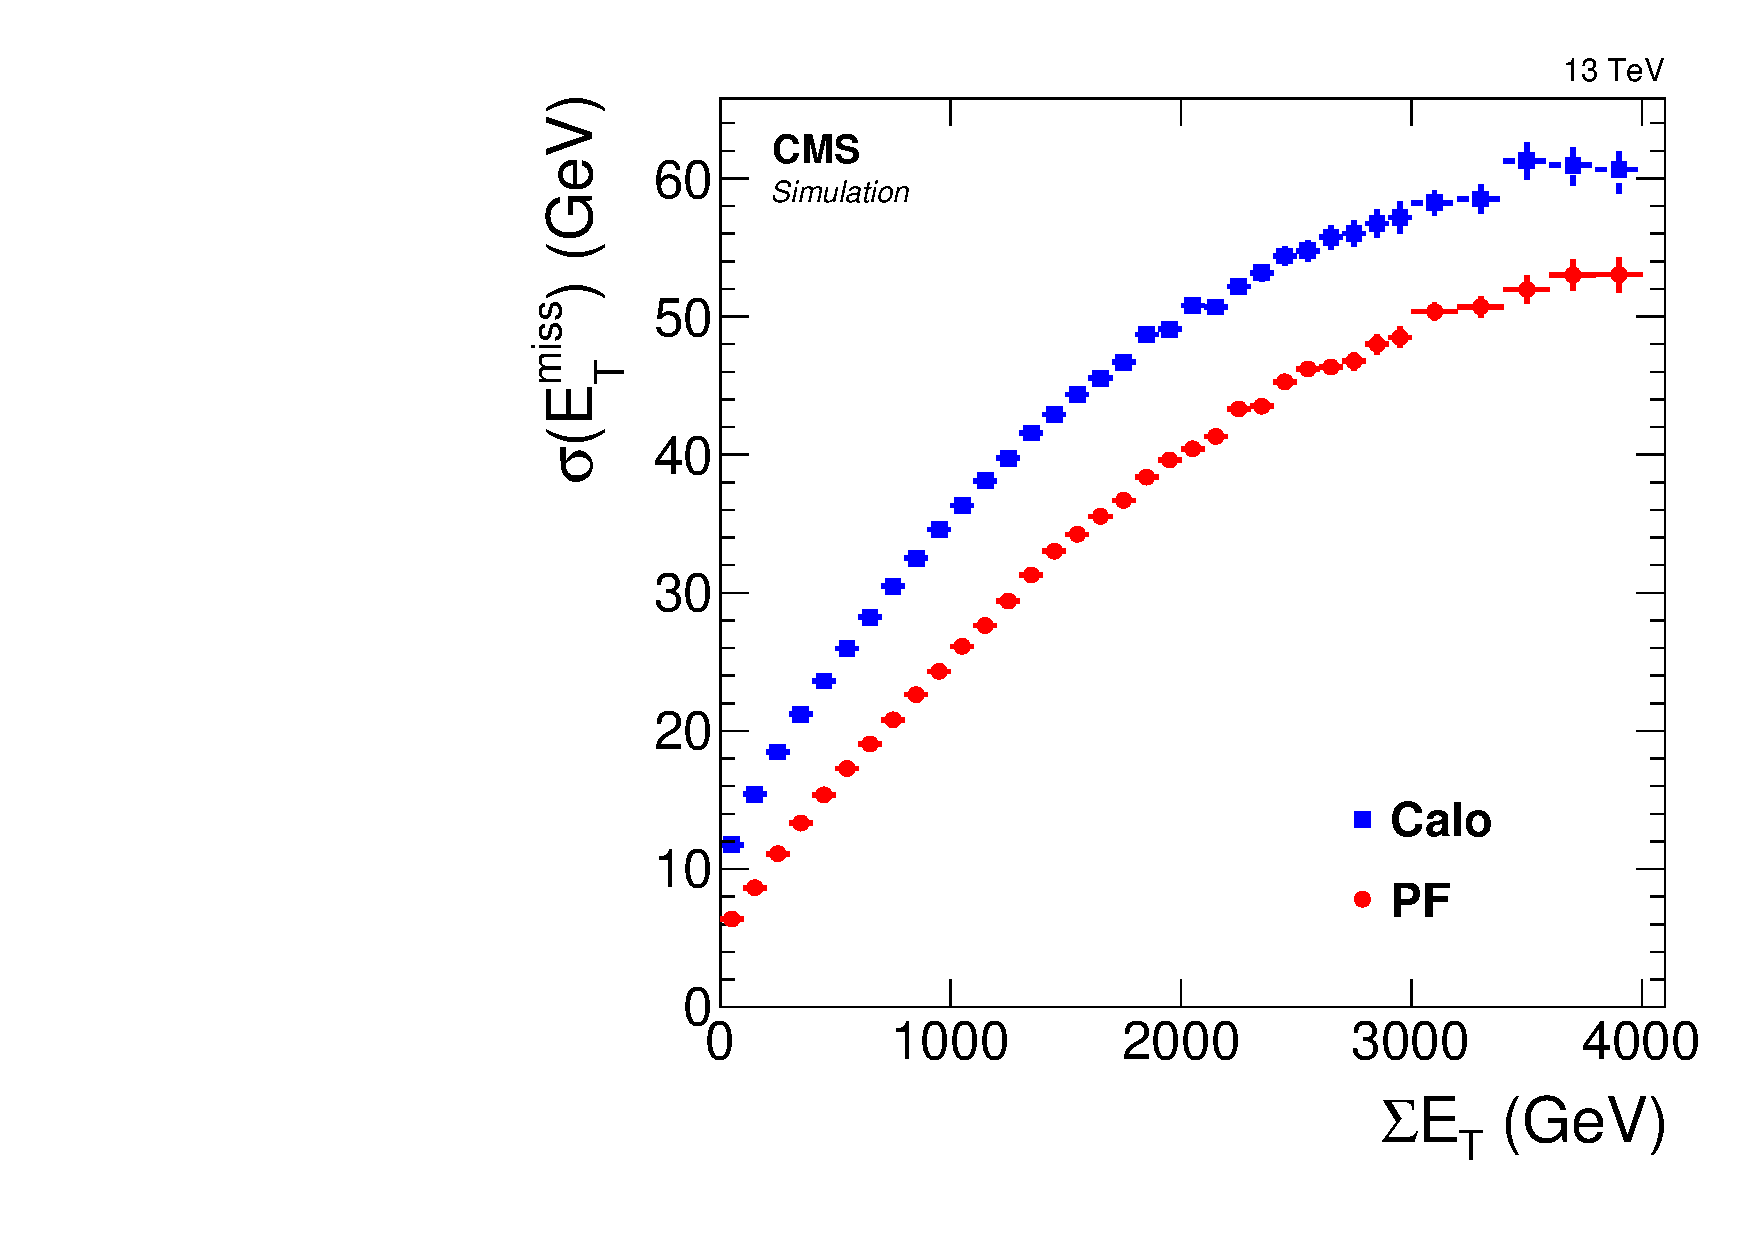
\includegraphics[width=0.45\textwidth]{figs/cms/met_sigma_vs_sumet.pdf}
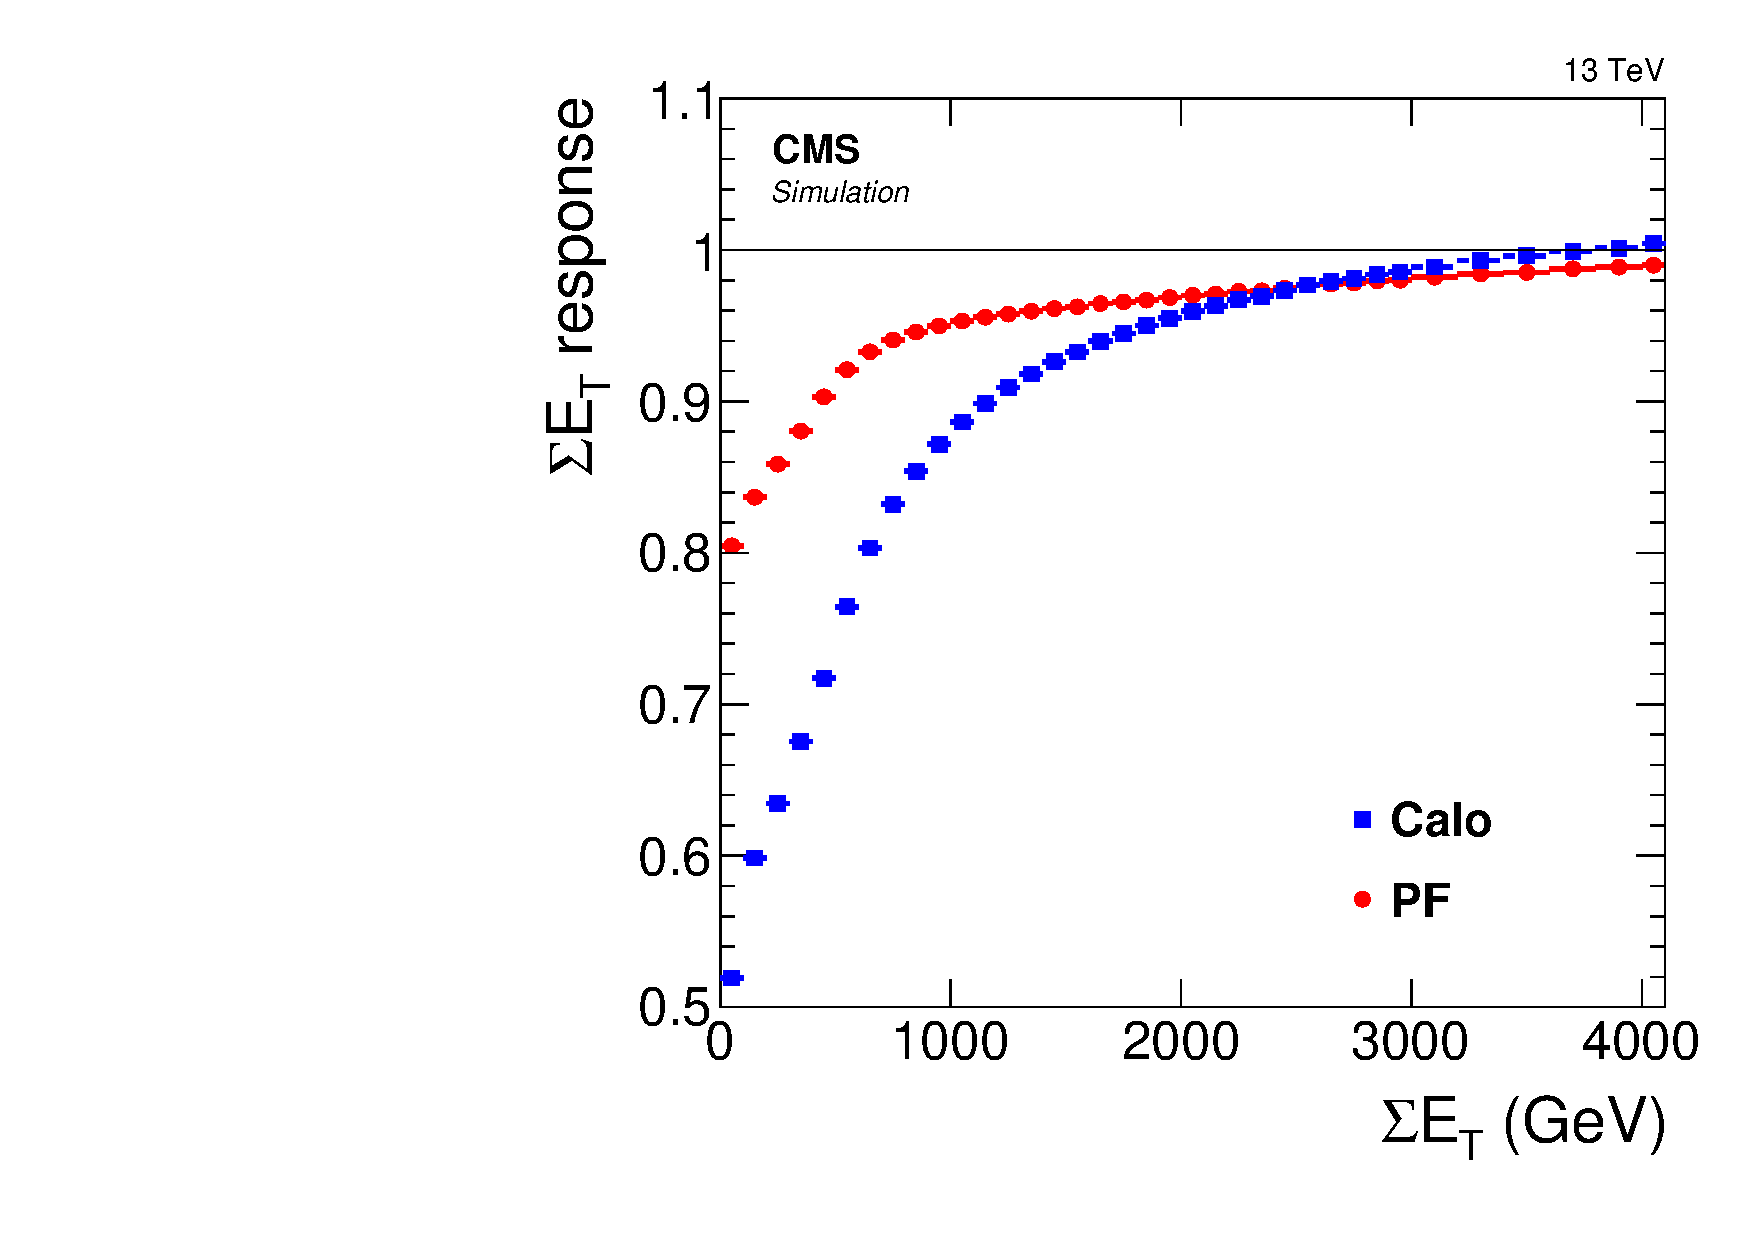
\includegraphics[width=0.45\textwidth]{figs/cms/met_response_vs_sumet.pdf}
\caption{Absolute \MET resolution (left) and \sumET response (right) for a simulated QCD multijet sample.
In the case of the particle flow estimate, \MET stands for $\MET ({\mathrm{PF}})$ and \sumET for $\sumET ({\mathrm{PF}})$. In the case of the calorimeter-based estimate, they stand for $\MET ({\mathrm{Calo}})$ and $\sumET ({\mathrm{Calo}})$.\label{fig:expected_performance_met}}
\end{figure}

\begin{figure}[htbp]
\centering
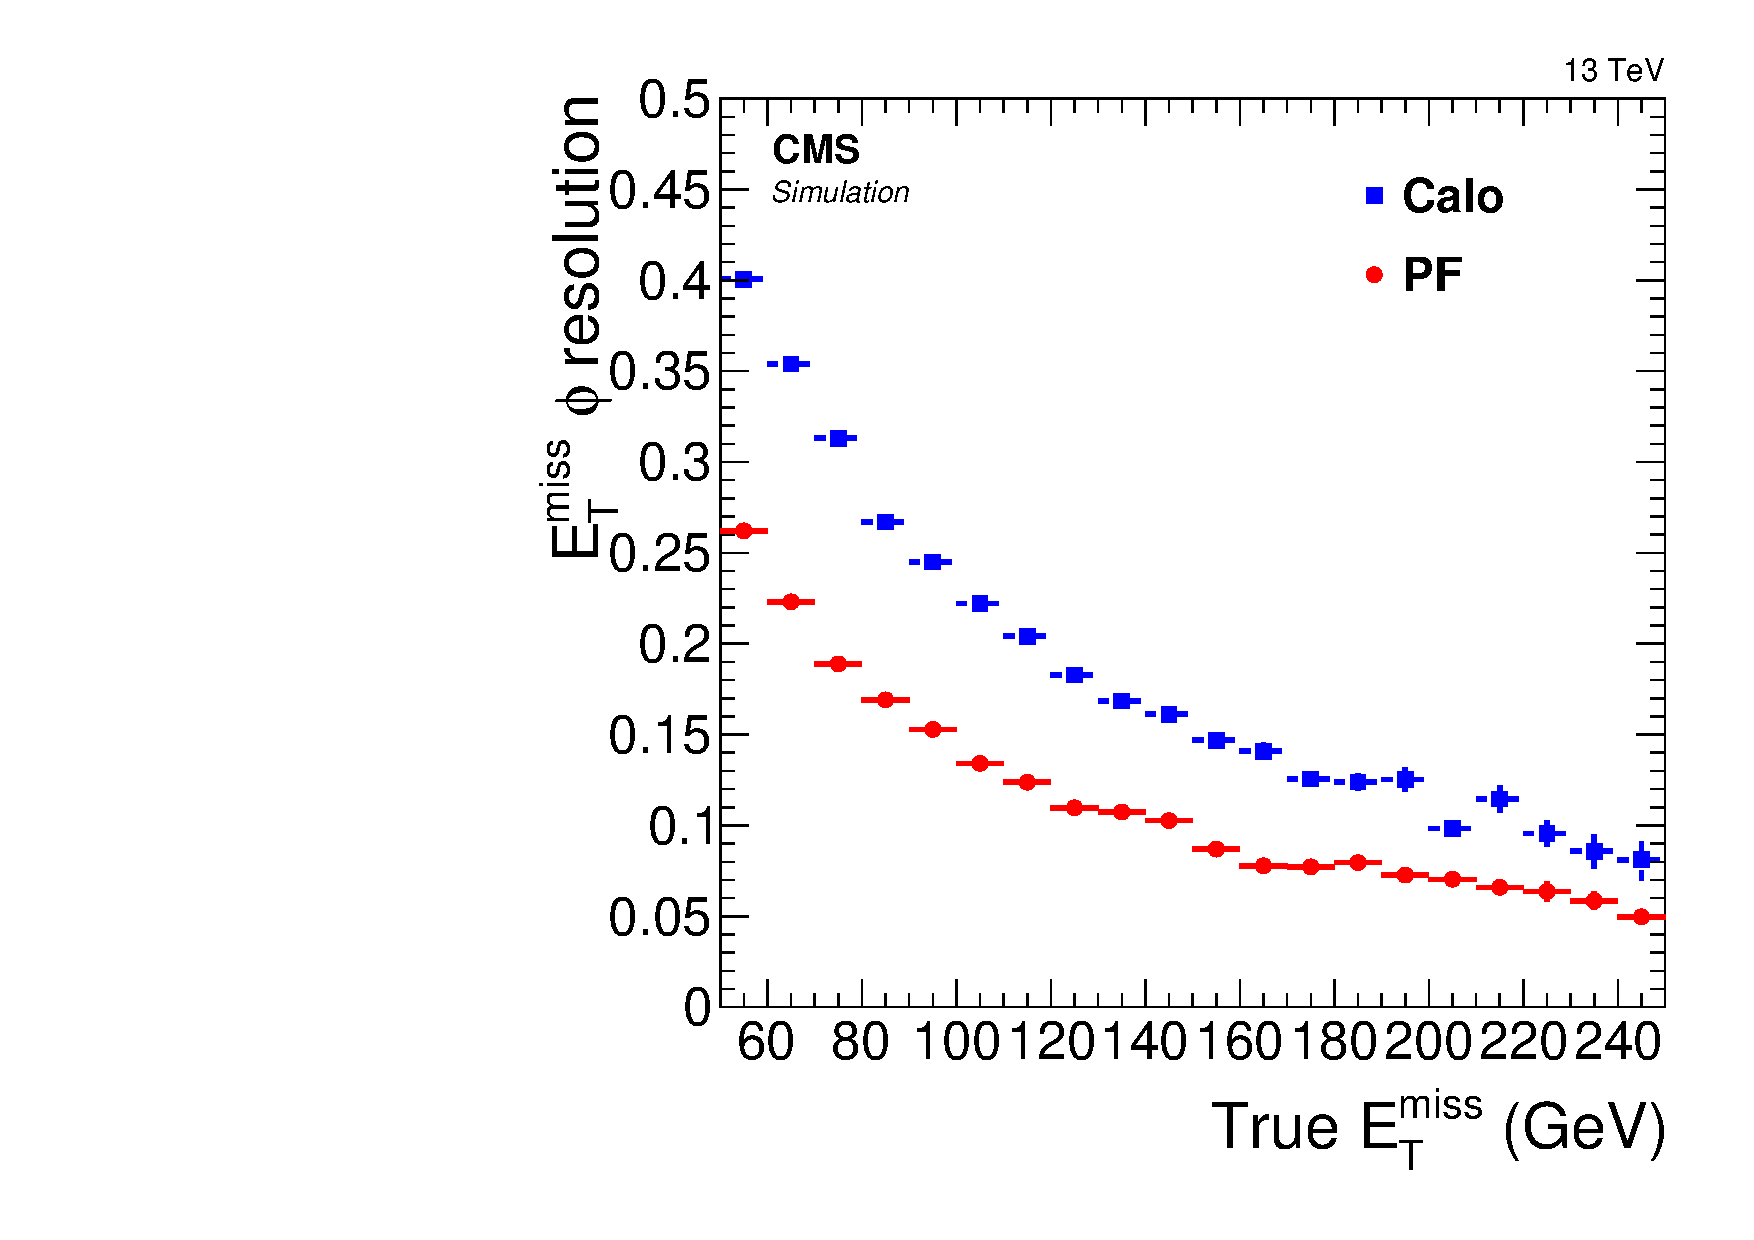
\includegraphics[width=0.49\textwidth]{figs/cms/met_phi_vs_truemet.pdf}
\caption{
Resolution on the measurement of the \vecMET azimuthal angle as a function of the true \MET for a simulated \ttbar sample.
\label{fig:expected_performance_met_phi_resolution}}
\end{figure}

Rare failures related to the detector, the reconstruction of the PF inputs, 
and the algorithm itself generally translate to unexpectedly large values of the \MET.
Events with such large values are systematically scrutinised and when a shortcoming of the PF algorithm is fixed, 
the global performance of the PF reconstruction typically improves as a whole population of events were affected at lower values
of the \MET. 

The performance of \VEtmiss reconstruction with all corrections
applied is assessed with a sample
of observed events selected in the dimuon final state that is
dominated by events with a $\cPZ$ boson decaying to two
muons~\cite{Khachatryan:2014gga}. The dataset is collected with a
trigger requiring the presence of two muons passing \pt thresholds of
17 and 8\GeV, respectively. The two reconstructed muons must fulfill $\pt > 20 $\GeV and $|\eta| <
2.1$, satisfy isolation requirements, and have opposite charge. Events where the invariant mass of the dimuon system is outside the
window $60<m_{\mu\mu}<120$\GeV are rejected.
%The expression of $\vecMET (\mathrm{PF})$, defined above, includes a
%correction term accounting for the response of the jets in the final
%state. Here, two additional terms are introduced, the first to correct
%for the presence of many low-energy particles from pileup
%interactions, and a second one to correct for an observed $\Phi$
%asymmetry due to a shift in $\vecMET (\mathrm{PF})$ along the detector
%$x$ and $y$ axes.
Figure~\ref{fig:met_distribution} shows the spectrum
of $\MET ({\mathrm{PF}})$ in the $\cPZ\rightarrow\mu\mu$ event sample. The
simulation describes the observed distribution over more than five
orders of magnitude.

\begin{figure}[htp]\centering
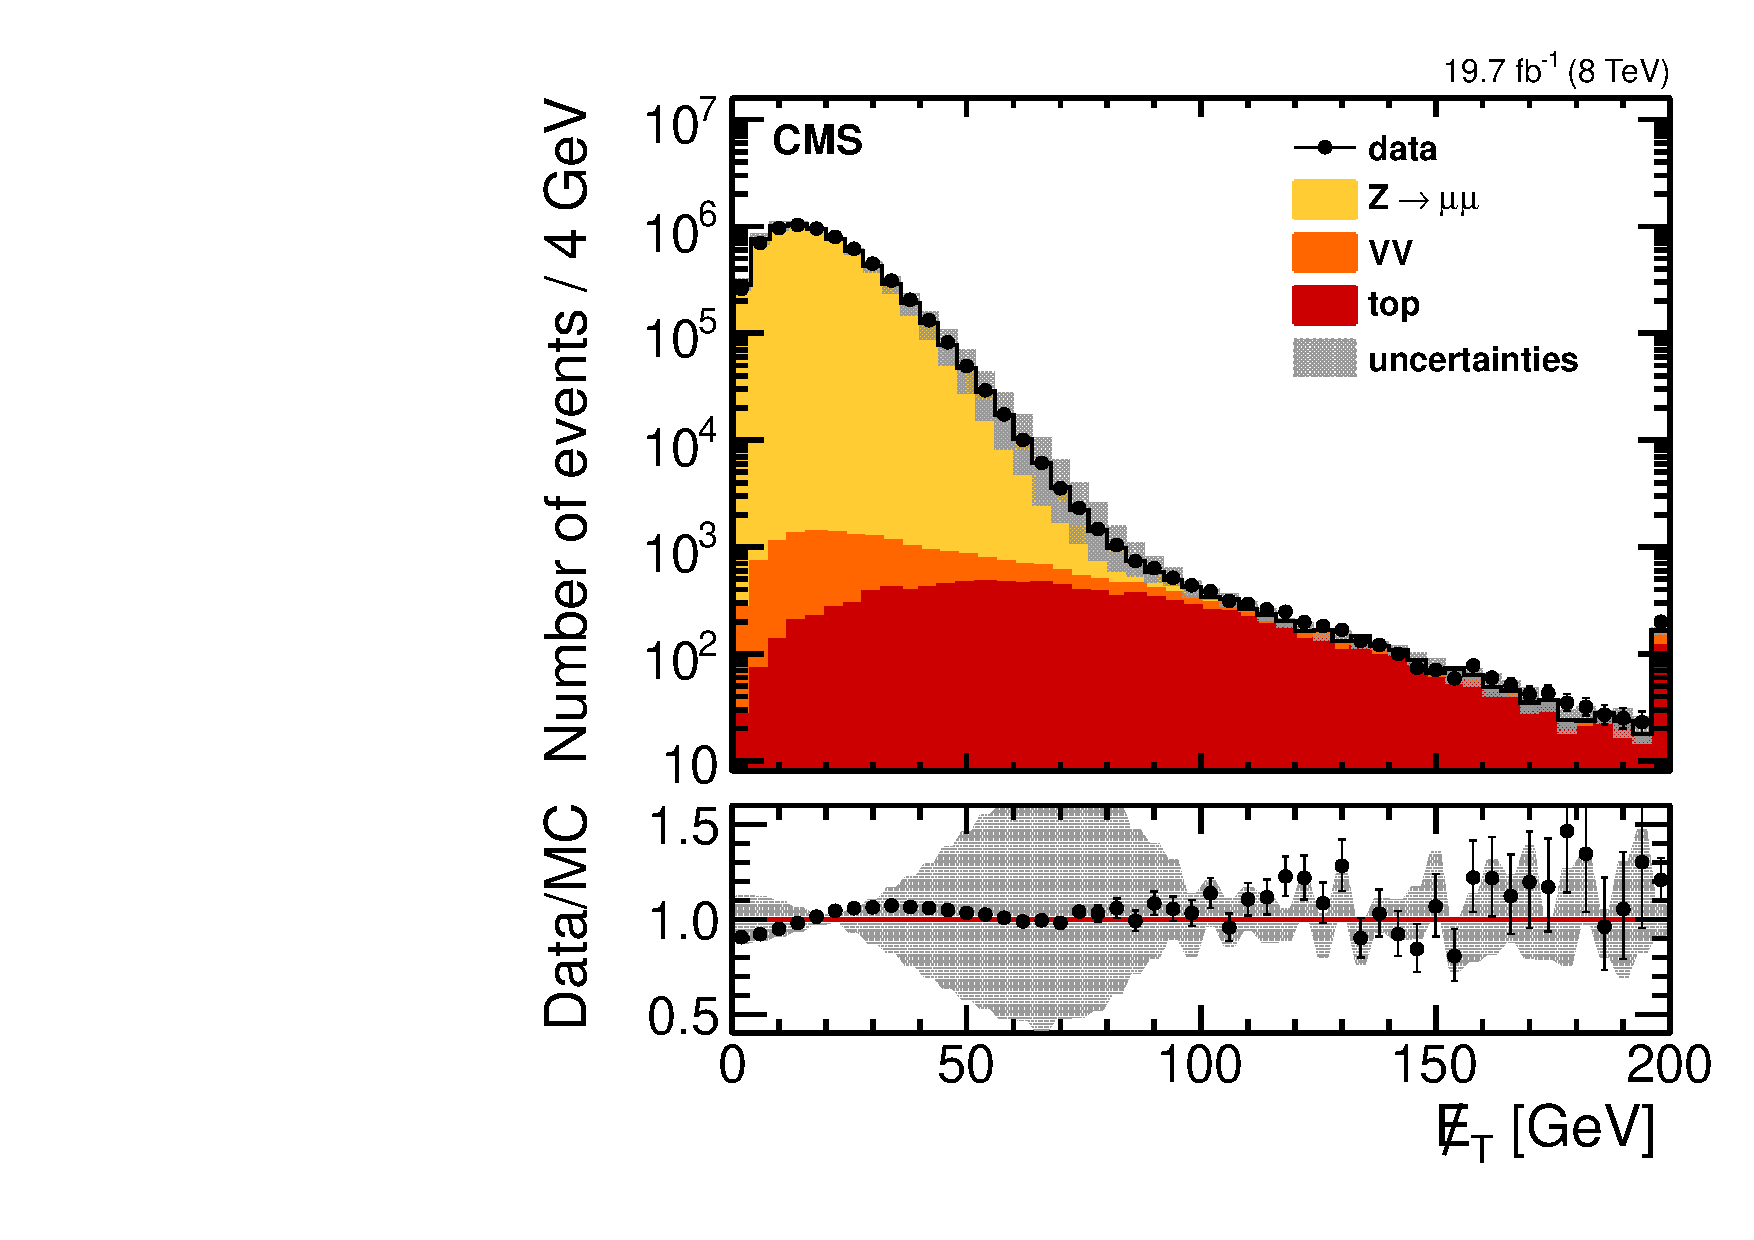
\includegraphics[width=.7\linewidth]{figs/cms/pFlowPFMET.pdf}
\caption{Spectrum of $\MET (\mathrm{PF})$ in the $\cPZ\rightarrow\mu\mu$ dataset.
The observed data are compared to simulated $\cPZ\rightarrow\mu\mu$,
diboson (VV), and $\ttbar$ plus single-top-quark events (top).
The lower frame shows the ratio of data to simulation, with the
uncertainty bars of the points including the statistical uncertainties
of both observed and simulated events and the grey uncertainty band
displaying the systematic uncertainty of the simulation. The last bin contains the overflow.\label{fig:met_distribution}}
\end{figure}

\subsection{Identification of \PQb-quark Jets}
\label{sec:btag}
Jets that arise from bottom-quark hadronization (\cPqb-jets) are
present in many physics processes, such as the decay of top quarks,
the Higgs boson, and top and bottom squarks predicted by natural supersymmetric models. 
The ability to accurately identify \cPqb-jets is crucial in reducing
the otherwise overwhelming background to these channels from processes
involving jets from gluons (\cPg) and light-flavor quarks (\cPqu,
\cPqd, \cPqs), and from \cPqc-quark fragmentation. 

The properties of the bottom and, to a lesser extent, the charm
hadrons can be used to identify the hadronic jets into which the
\cPqb\ and \cPqc\ quarks fragment.  These hadrons have relatively
large masses, long lifetimes ($c\tau\sim 450~\mu\mathrm{m}$) and daughter particles with hard momentum
spectra. Their semileptonic decays can be exploited as well.

A variety of reconstructed objects -- tracks, vertices and identified
leptons -- can be used to build observables that discriminate between
\Pqb- and light-parton jets. Several simple and robust algorithms use
just a single observable, while others combine several of these
objects to achieve a higher discrimination power. Each of these
algorithms yields a single discriminator value for each jet. The
minimum thresholds on these discriminators define loose (``L''), medium
(``M''), and tight (``T'') operating points with a misidentification
probability for light-parton jets of close to 10\%, 1\%, and 0.1\%,
respectively, at an average jet \pt of about $80 \GeV$.

The algorithm that was shown to have the best performance
in terms of \cPqb-jet identification efficiency and light-parton-jet fake rate
in Run 1 is the \emph{Combined Secondary Vertex} (CSV)
algorithm, which makes use of multivariate techniques to combine
discriminating variables built from displaced track and secondary
vertex information as well as jet
kinematics~\cite{btag7TeV,btag8TeV}. In short, the following set of
variables with high discriminating power and low correlations is used
(if no secondary vertex is reconstructed, only the last two variables are available): 
\begin{itemize}
\item the vertex category (real, ``pseudo,'' or ``no vertex'');
\item the flight distance significance (ratio of the flight
  distance to its estimated uncertainty) in the transverse plane (``2D'');
\item the vertex mass;
\item the number of tracks at the vertex;
\item the ratio of the energy carried by tracks at the vertex with respect to all tracks in the jet;
\item the pseudorapidities of the tracks at the vertex with respect to the jet axis;
\item the 2D impact parameter (IP) significance (ratio of the IP to its estimated uncertainty, ) of the first track that raises the invariant mass above the charm threshold of $1.5 \GeV$ (tracks are ordered by decreasing IP significance and the mass of the system is recalculated after adding each track);
\item the number of tracks in the jet;
\item the 3D IP significances for each track in the jet.
\end{itemize}
Two likelihood ratios are built from these variables to
discriminate between \cPqb-  and \cPqc-jets and between \cPqb\ and
light-parton jets. They are combined with prior weights of $0.25$ and $0.75$, respectively.

The \cPqb-jet identification
efficiency is about 70\% for a misidentification probability for
light-parton jets of about 1\% for jets with \pt between $80$ and $120 \GeV$,
as seen in Fig.~\ref{fig:mcPerformance}.
For Run 2, the CSV algorithm was significantly improved (CSVv2) by
updating the multivariate algorithm from a simple likelihood
ratio to a neural network, improving the track selection and
adding new variables, and using a new algorithm for the
reconstruction of the secondary vertices, the so-called Inclusive
Vertex Finder (IVF).  These updates turn into a net improvement in
performance of about a 10\% increase in the \cPqb-jet identification
efficiency at a 1\% of light-parton-jet misidentification rate, as pictured
in Fig.~\ref{fig:mcPerformance2015}. The \cPqb-jet identification at
HLT uses the same algorithm as in the offline reconstruction, optimized to reduce the execution time~\cite{Tosi:2015zhy}. 
%This was achieved thanks to a more extensive use of the Iterative Tracking reconstruction in the regions-of-interest, which helps in reducing the combinatorics. The second goal is to improve the performance of the online version of the b-tagging algorithm. This was achieved thanks to the Iterative Tracking reconstruction, to the new implementation of the b-tagging algorithm (CSVv2+IVF) and to a better resolution on the position of the primary vertex. By using tracks from the Iterative Tracking, and performing the vertex fitting with an Adaptive Vertex Fitter [6] where the track clustering is made with a Deterministic Annealing (DA) algorithm [7], indeed, the resolution on the position of the primary vertex along the z-axis is about 20-30 μm.

\begin{figure}
\centering
\subfigure{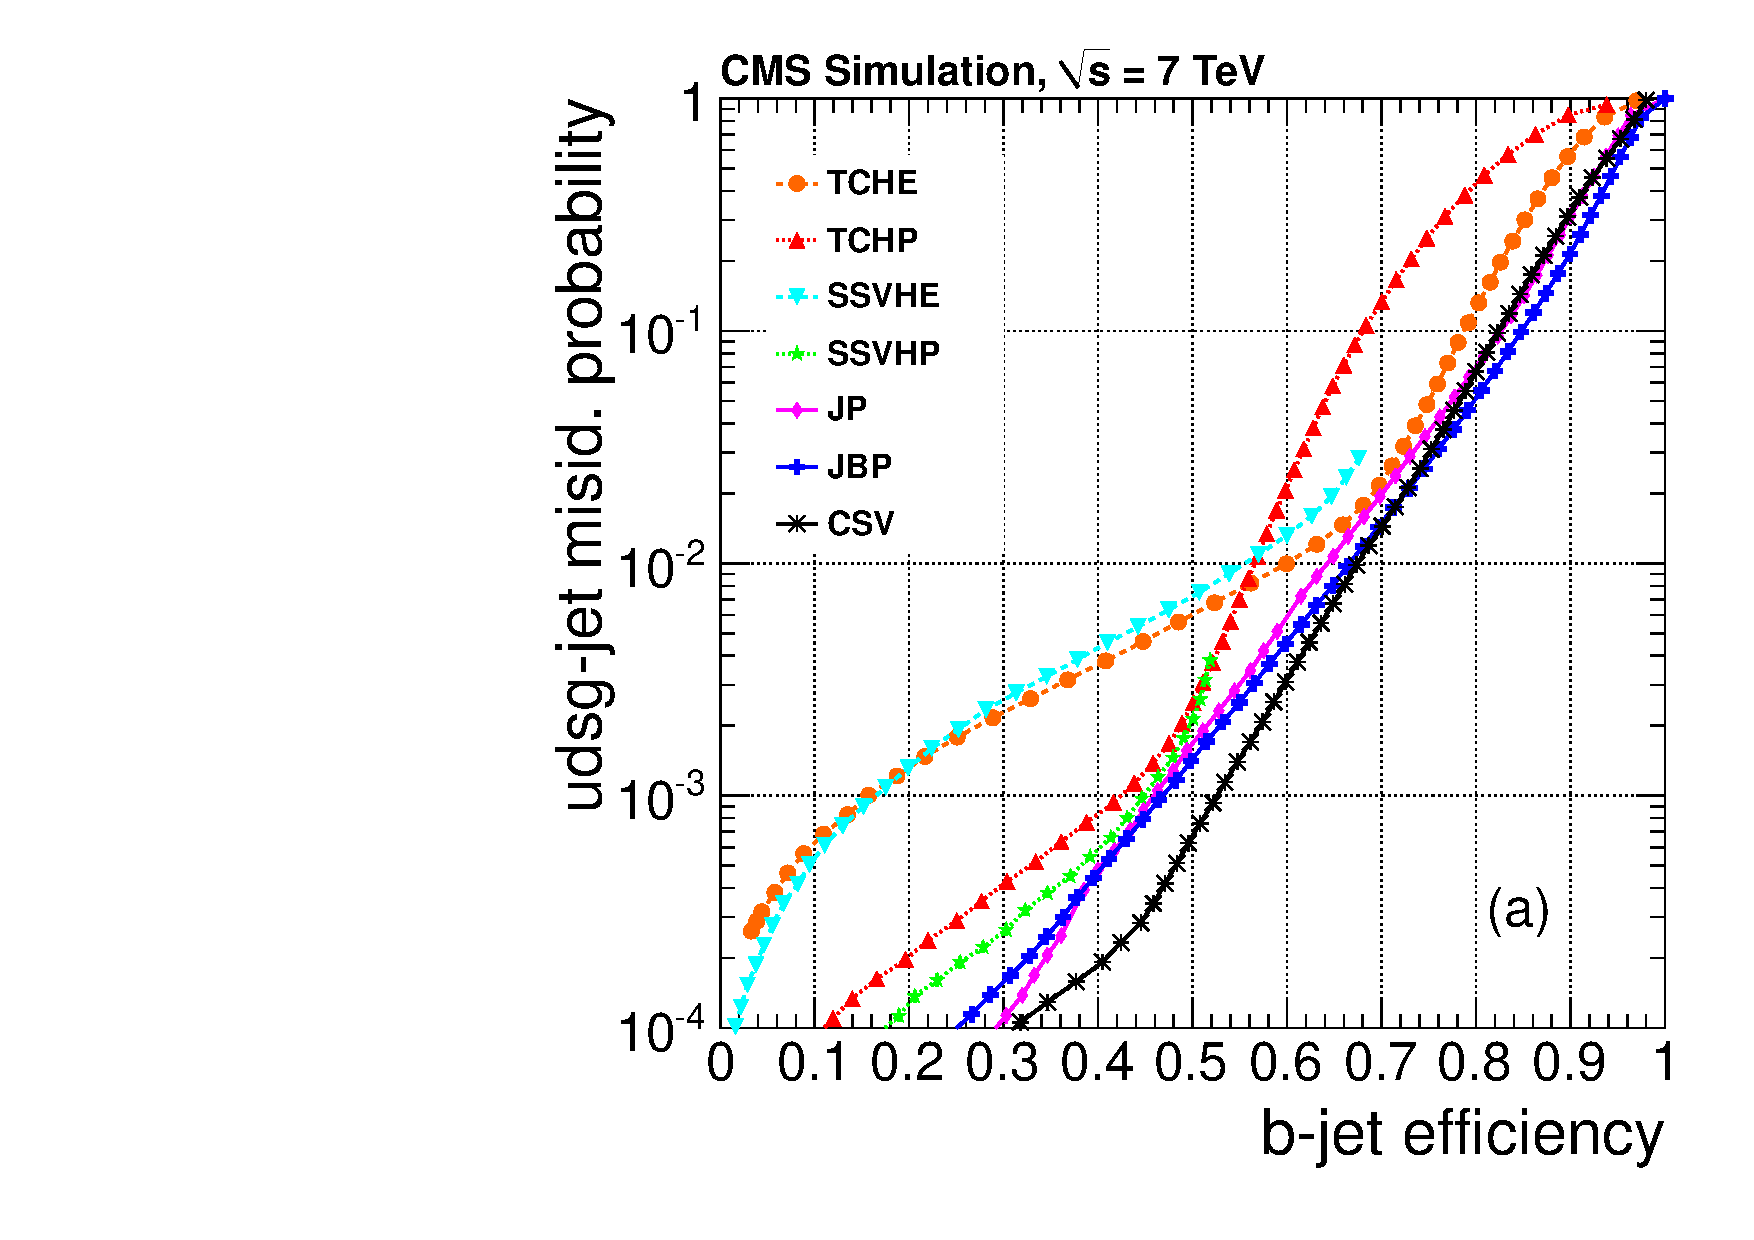
\includegraphics[width=0.45\textwidth]{figs/cms/Combined_udsgvsb_Efficienies.pdf}}
\subfigure{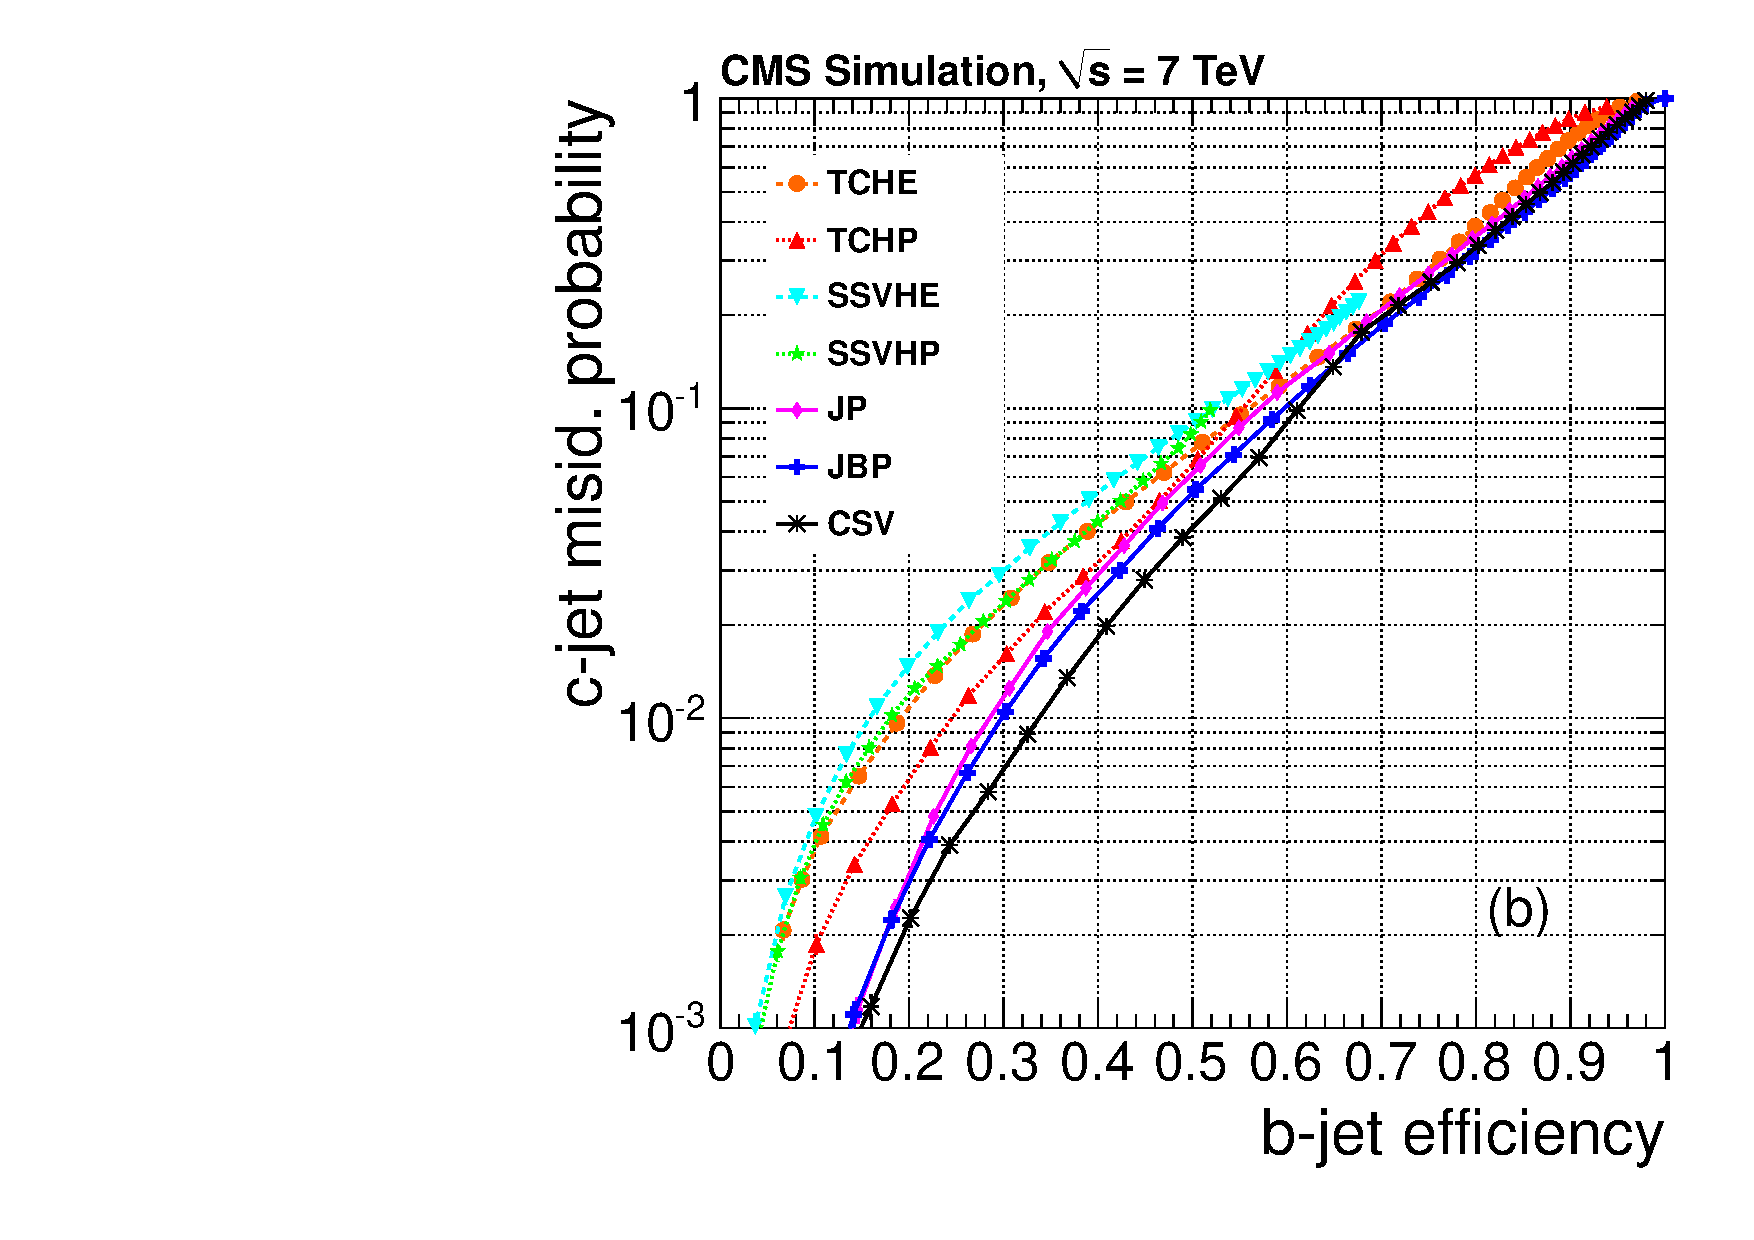
\includegraphics[width=0.45\textwidth]{figs/cms/Combined_cvsb_Efficienies.pdf}}
\caption{
Performance curves obtained from simulation for the different
\cPqb-jet tagging algorithms. Light-parton- (left) and \cPqc-jet (right) misidentification probabilities as a function of the \cPqb-jet efficiency.  Jets with $\pt > 60\GeV$ in a sample of simulated multijet events are used to obtain the efficiency and misidentification probability values.
\label{fig:mcPerformance}}
\end{figure}

\begin{figure}
\centering
\subfigure{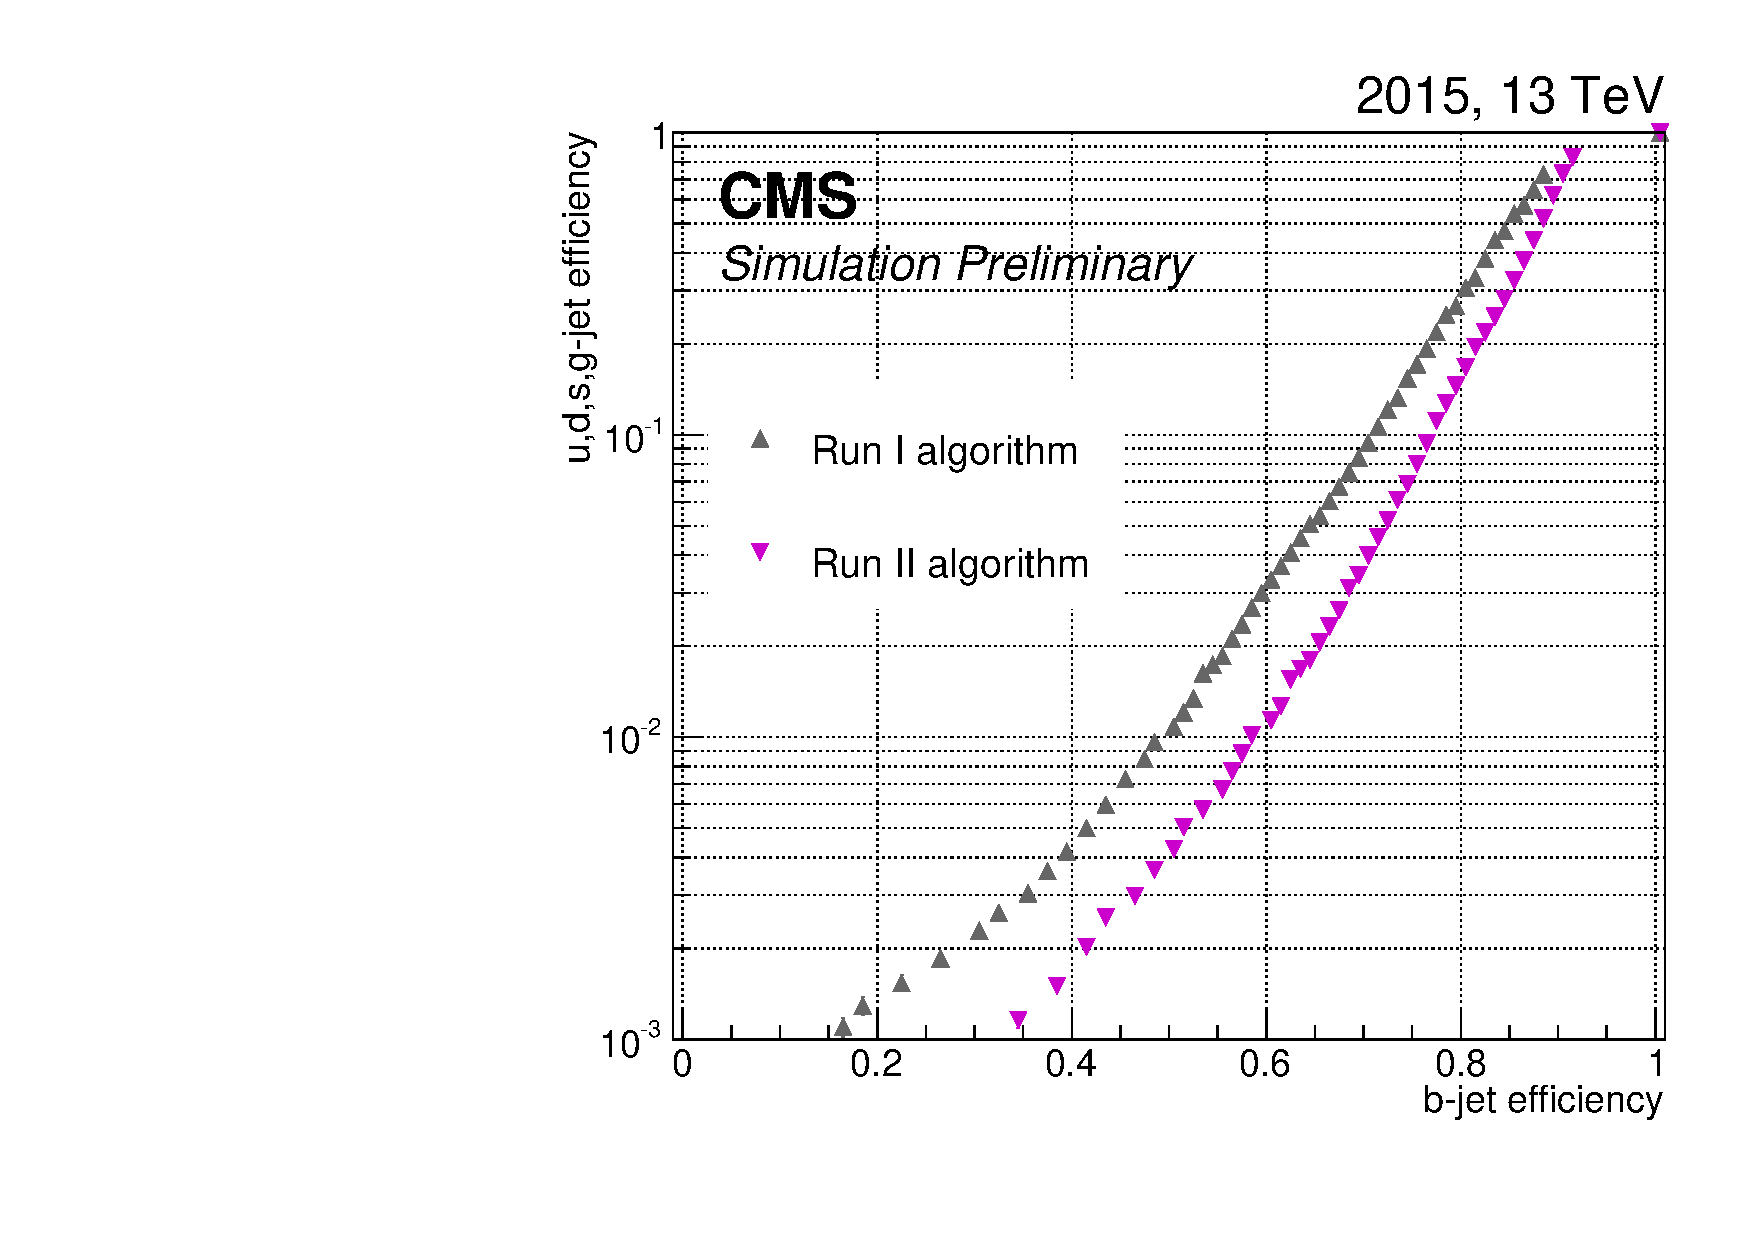
\includegraphics[width=0.45\textwidth]{figs/cms/b_udsg_RunI-II_ttbar_PU40_bx25.pdf}}
\subfigure{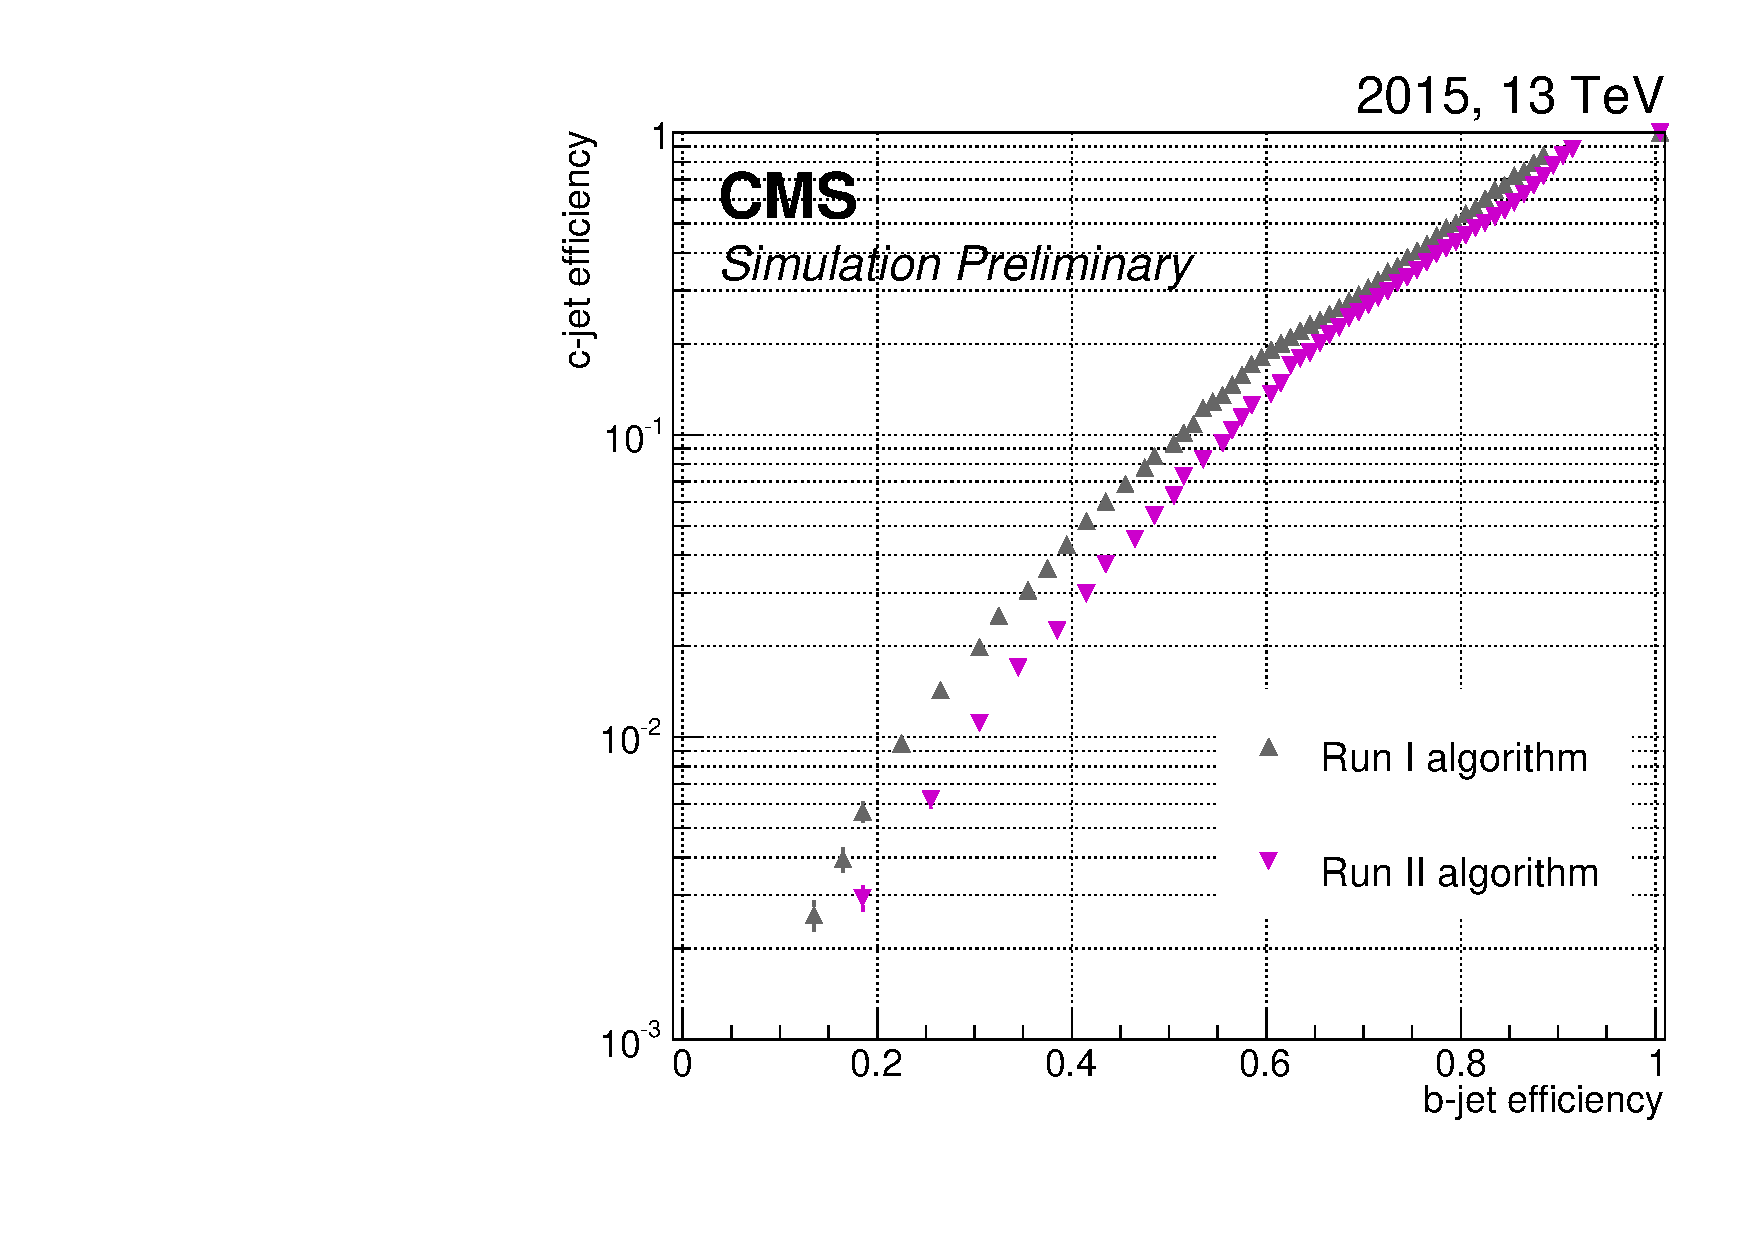
\includegraphics[width=0.45\textwidth]{figs/cms/b_c_RunI-II_ttbar_PU40_bx25.pdf}}
\caption{
Light-parton- (left) and \cPqc-jet (right) misidentification
probabilities as a function of the \cPqb-jet efficiency for the
\cPqb-jet tagging algorithms used at HLT. The gray and
magenta curves show the performance of the Run 1 and Run 2 algorithms,
respectively. 
%The Run 1 algorithm uses primary vertices made out of pixel tracks and CTF tracks as input to the CSV
%algorithm while the Run II algorithm uses iterative tracks and deterministic annealing primary vertices made out of iterative tracks
%as input to the CSVv2+IVF algorithm. 
Jets from simulated \ttbar events at $\sqrt{s} = 13$ \TeV with 40
average pileup interactions and a bunch spacing of 25 \unit{ns} are considered. 
\label{fig:mcPerformance2015}}
\end{figure}


% INFOS FROM SIMONE, DON'T REMOVE
%
% limitations of the HLT
%  time
%  paths should be independent
% 
% Even the regional tracking cannot work. 
% select events from a given L1 seed
% reconstruct calo based quantities with the same algorithms as offline
% each path defines calo-based selection, and then pf-based selection
%    so e.g. if calo MET > 80, then tracking, PF, then cut on PFMET
%
% tracking:
% reconstruct all pixel tracks as in offline (tight selections, narrow vertices)
% vertices from pixel tracks 
% take the first 3 or 4 vertices (sumpt2 + other ranking criteria)
%
% reconstruct tracks from all of these vertices and to the interesting regions. 
% 0 : start from all pixel tracks from subsample of vertices - no regions 
% 1 : define regions in which we have isolated tracks from previous iteration. 
%     combine with calo jet regions (now regional, still from same vertices)
% 2 : rinse and repeat 1 with looser seeding conditions.  


\section {Level-1 and High-Level Trigger}
\label{sec:trigger}

The role of the trigger is to reduce the rate of recorded collision to
a level which is manageable by the following data acquisition (DAQ)
and online reconstruction. At the LHC, the proton beams are organized in
bunches separated in time by 50 \unit{ns} during Run 1 (2010-2013) and 25 \unit{ns}
during Run 2 (2015-present), implying a collision rate on the order of
40 \unit{MHz}.
%in reality a bit less, because not all bunches in the machine are filled with protons
The maximum acceptable rate for data acquisition and storage is of the order of 1 \unit{kHz}, and
the trigger is designed to reduce the rate to that level, while
maintaining the largest possible acceptance of interesting physics signal
events from the collisions and efficiently rejecting the
non-interesting ones. Figure~\ref{fig:streams}

\begin{figure}\centering
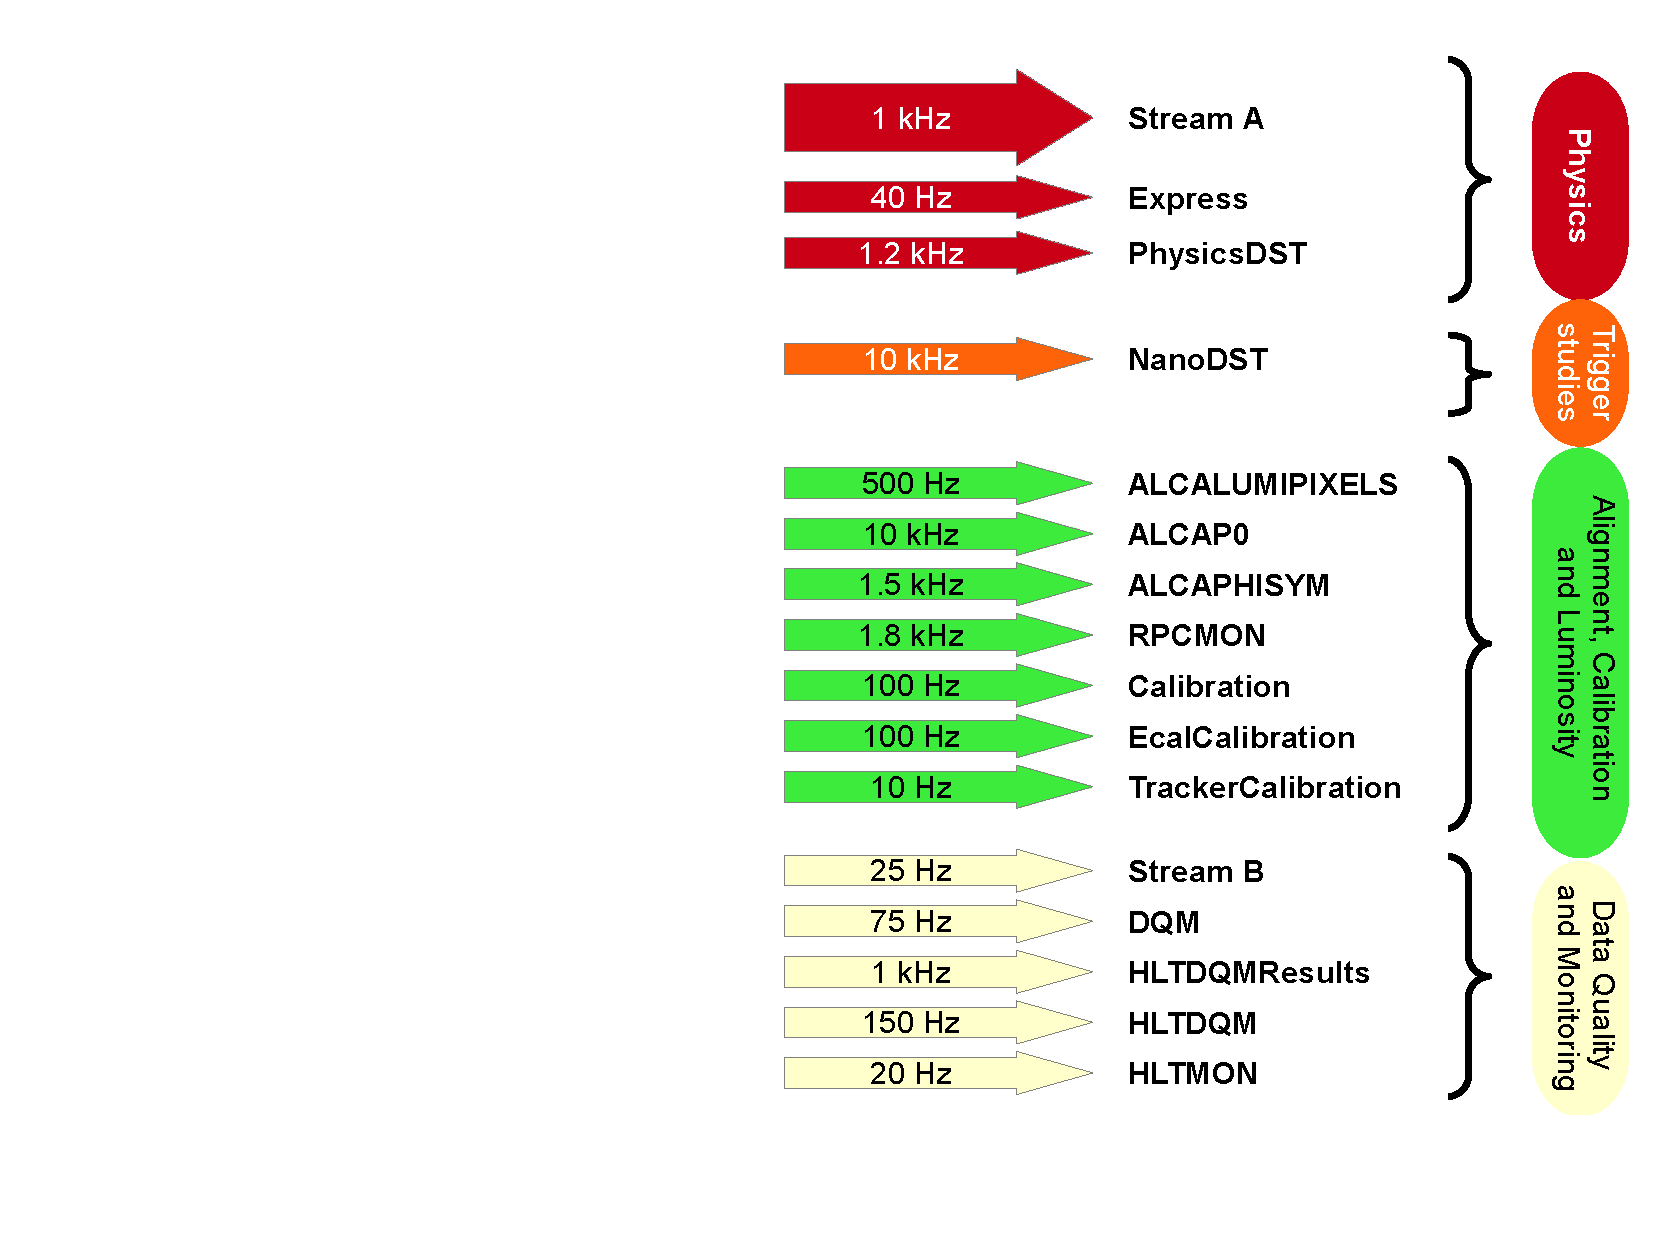
\includegraphics[width=.45\textwidth]{figs/cms/Streams2012.pdf}
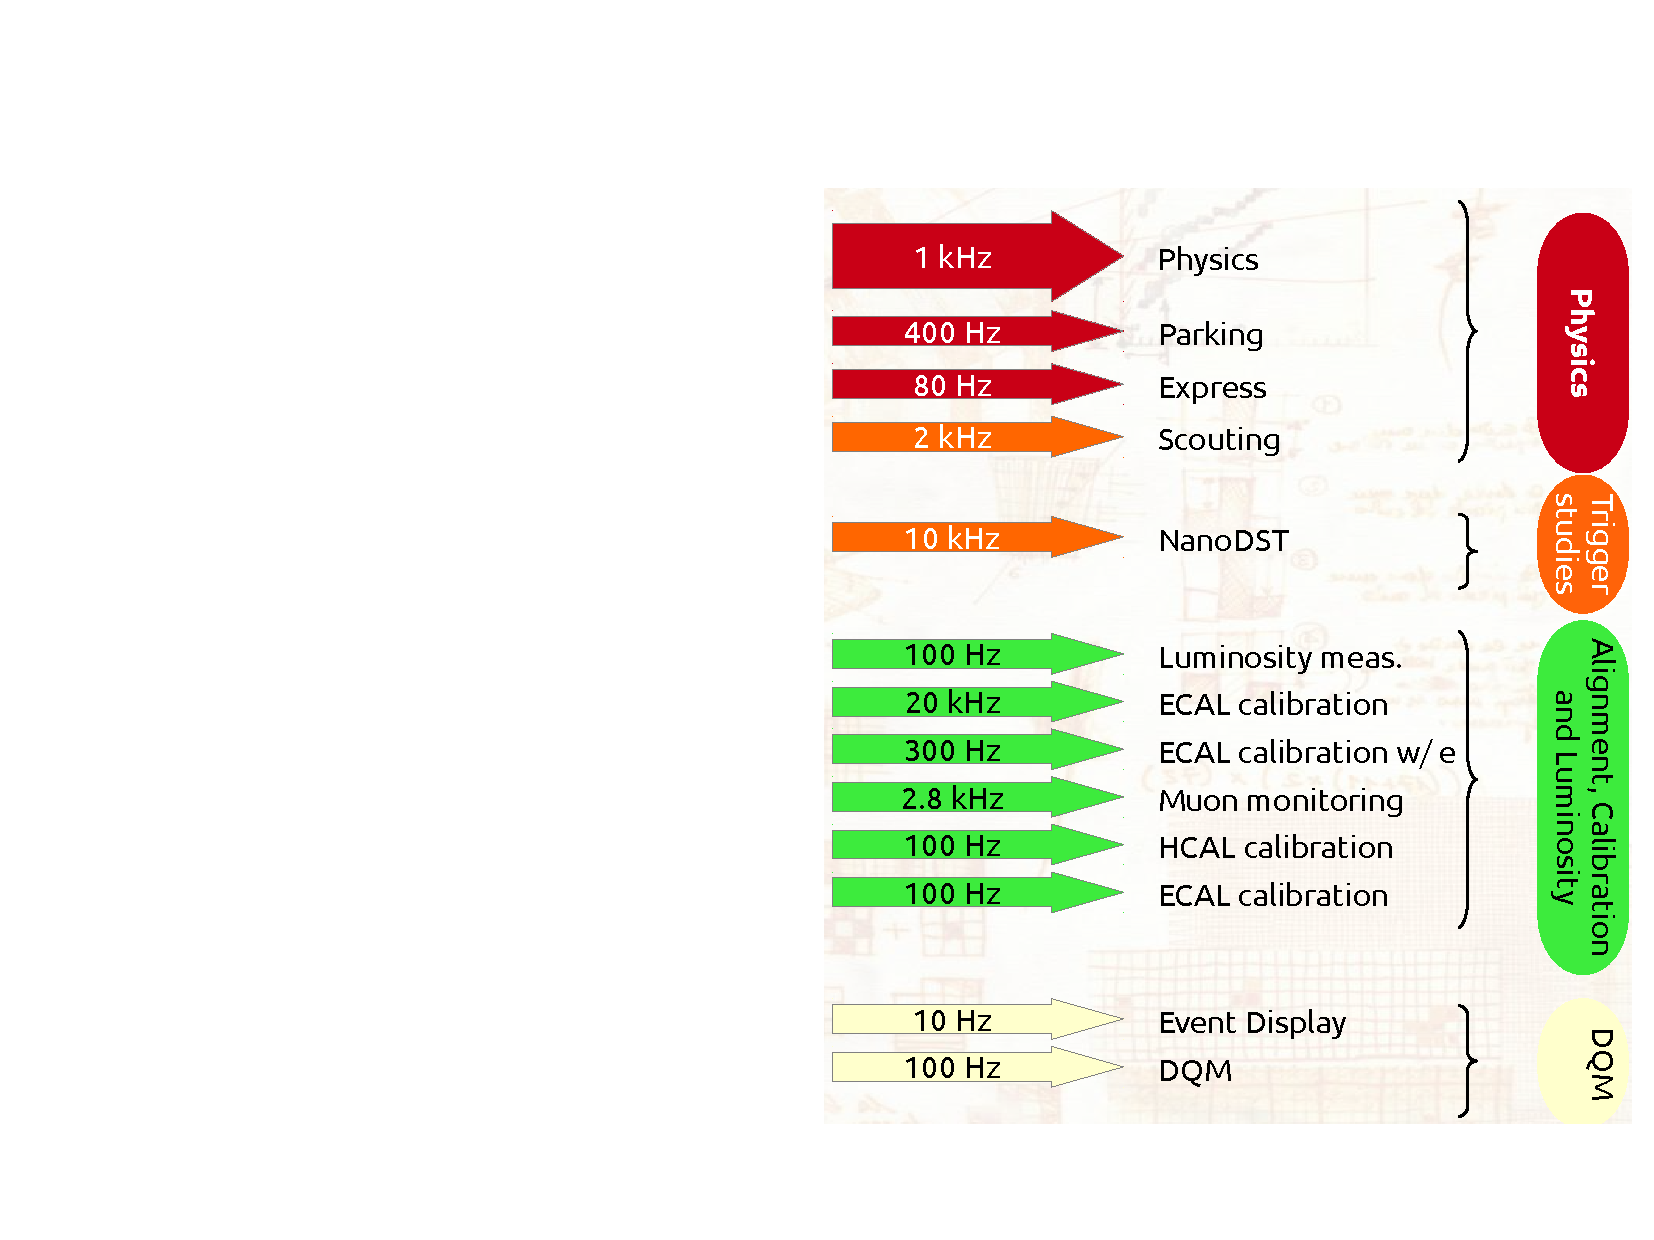
\includegraphics[width=.45\textwidth]{figs/cms/Streams2015.pdf}
\caption{Data streams during 2012 (left) and 2015 (right)
\label{fig:streams}}
\end{figure}

The design chosen for the trigger of the CMS experiment is a two-level system. The
Level 1 (L1) trigger is based on FPGA and custom ASIC technology and uses information
from the calorimeters and muon spectrometers of the experiment in order to accept or reject
an event; it reduces the event rate down to approximately 100 \unit{kHz}, acceptable by the readout
electronics. The High-Level Trigger (HLT) is implemented in software running on a farm of
commercial computers which includes approximately 16,000 CPU cores, and reduces the L1 output rate
to the sustainable level for storage and physics analysis of about 1 \unit{kHz}. The HLT software
consists of a streamlined version of the offline reconstruction
algorithms; it exploits the same software used for offline
reconstruction and analysis, optimized in order to comply with the
strict time requirements of the online selection.

The L1 trigger decision is made within a fixed time
interval of less than 4 $\mu\mathrm{s}$. The operational L1 output
rate of 100 \unit{kHz}, together with the number of CPUs in the HLT
farm, imposes a fundamental constraint on the amount of time available for the HLT to process events.
Exceeding this limit impacts the ability of CMS to collect data
efficiently. Given the CPUs available in 2015, the timing budget of the HLT is
measured to be about 300\unit{ms} when the machines are fully loaded
(or 160\unit{ms} when the machines are running a single
job)~\cite{Richardson:2015zdg}.

The HLT menu in CMS has a modular structure, which is graphically depicted in Fig~\ref{fig:modular}.
The menu is subdivided into logically independent paths, which may be
run in parallel; more than 400 different HLT paths are used for Run 2
data taking. Each path is a sequence of
reconstruction modules (producers) and filtering modules
(filters). Filters typically select events based on the properties of a given physics object (photons, electrons,
muons, jets, \ptvecmiss, \PQb-tagged jets, etc.), or, as in the case of the razor triggers
detailed in Ch.~\ref{ch:hlt13TeV}, the properties of a combination of physics objects
along with the values of topological variables $\MR$ and  $\Rtwo$. The modules
within a path are arranged in blocks of increasing complexity, so that faster
algorithms are run first and their products are filtered: if a filter fails, the rest of the path is
skipped. 

%There are other important differences between the algorithms used at HLT and
%the ones used for the offline reconstruction, intended to reduce the CPU time consumption at
%HLT. For example, some online reconstruction algorithms have a specified regionality (detector read-out and reconstruction
%are restricted to narrow regions around the L1 or higher-level
%candidates), and the tracking and PF algorithms are simplified. 

\begin{figure}\centering
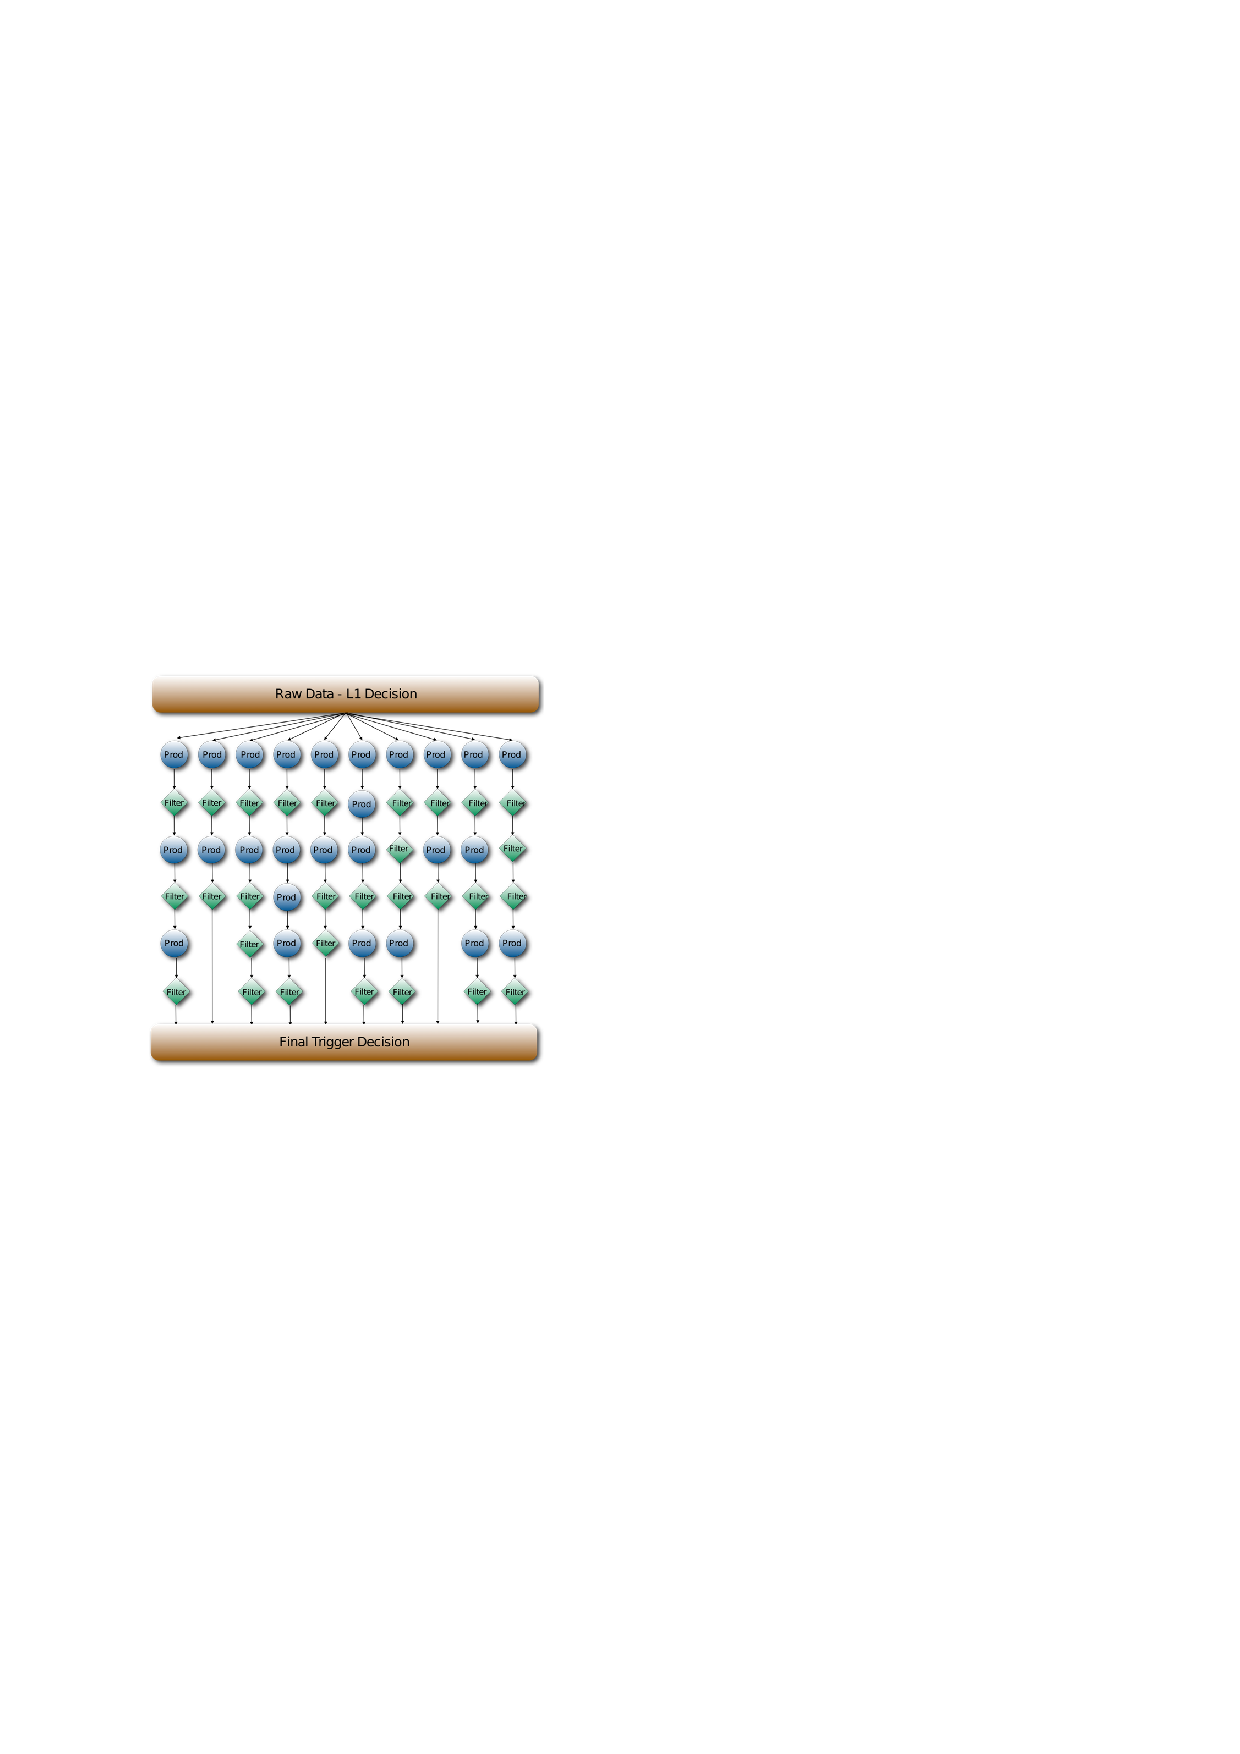
\includegraphics[width=.7\textwidth]{figs/cms/HLTschematic.pdf}
\caption{Schematic representation of the modular design of an HLT menu in CMS. The final trigger decision is the logical OR of the decisions of the single paths.
\label{fig:modular}}
\end{figure}

In order to keep the online reconstruction of physics objects at HLT as
close as possible to offline reconstruction, PF algorithms are used at
the HLT whenever possible. 
%to limit the triggering inefficiency and the false trigger rate
However, to stay within the HLT timing budget, the online
reconstruction of a single event for the HLT must be done more than one
hundred times faster than offline on average.
Offline, most of the processing time is spent reconstructing the inner
tracks for the PF algorithm. For the HLT, the tracking is reduced to three iterations, 
dropping the time-consuming reconstruction of tracks with a low
transverse momentum or arising from nuclear interactions in the
tracker material. These modifications preserve the reconstruction efficiency for
tracks with $\pt>0.8\,\GeV$ originating from the primary vertex, even
when these tracks are produced in the decay of a B hadron.
After track reconstruction, a specific instance of the particle identification and reconstruction algorithm runs online, 
with only two minor differences with respect to the offline algorithm:
the electron identification and reconstruction is not integrated in
the PF algorithm, and the reconstruction of nuclear interactions in the tracker is not performed.
The main effect of these modifications is a slightly higher jet energy
scale for jets featuring an electron or a nuclear interaction.


\subsection{Data Scouting}
\label{sec:scouting}

One of the main technical limitations of LHC data processing is the available bandwidth at which events can be
recorded on disk. Typically, this limitation forces the LHC experiments to increase the thresholds of their
triggers, in order to keep an acceptable data volume despite the increasing collision rate. 

An alternative strategy, referred to as \emph{data scouting}, is reducing the
event size from the default of $\sim 1$\unit{MB} in order to increase the recorded event rate. This
approach, first implemented at the LHC by the CMS experiment in
2011~\cite{CMS-DP-2012-022}, allows us to increase the physics signal
acceptance of CMS even in the presence of backgrounds with large cross
sections. This is particularly useful in the search for
narrow resonances in the dijet mass spectrum, as described in Ch.~\ref{ch:dijet}, where this strategy allows the search to
be extended into a low-dijet-mass region previously only accessible at
lower-energy colliders~\cite{Khachatryan:2016ecr,CMS-PAS-EXO-16-032}.

Fig~\ref{fig:DataScouting} schematically displays the $H_{\mathrm{T}}$
thresholds used for the different varieties of data scouting during the
2015 and 2016 runs and Fig~\ref{fig:DataScoutingContent} displays the
corresponding event content. \emph{Calo scouting}, which selects
events based only on Calo jets and records only calorimetric
information, has a very small event size of $\sim 1.5$\unit{kB}, allowing the
rate to go as a high as 3.8 \unit{kHz}. Meanwhile, \emph{PF scouting},
which runs the full PF algorithm and records all PF-reconstructed
information, including leptons, photons, and jets with \cPqb-tagging
information, has a larger event size $\sim 10$\unit{kB}. In order to stay within the
HLT timing budget, the maximum permissible rate is 720 \unit{Hz}. Simultaneously, the \emph{data parking} stream sends the
full raw events from PF scouting directly to tape without reconstruction. This
multifaceted approach is advantageous in the case that a signal is
seen in the scouting data that warrants more investigation.

\begin{figure}\centering
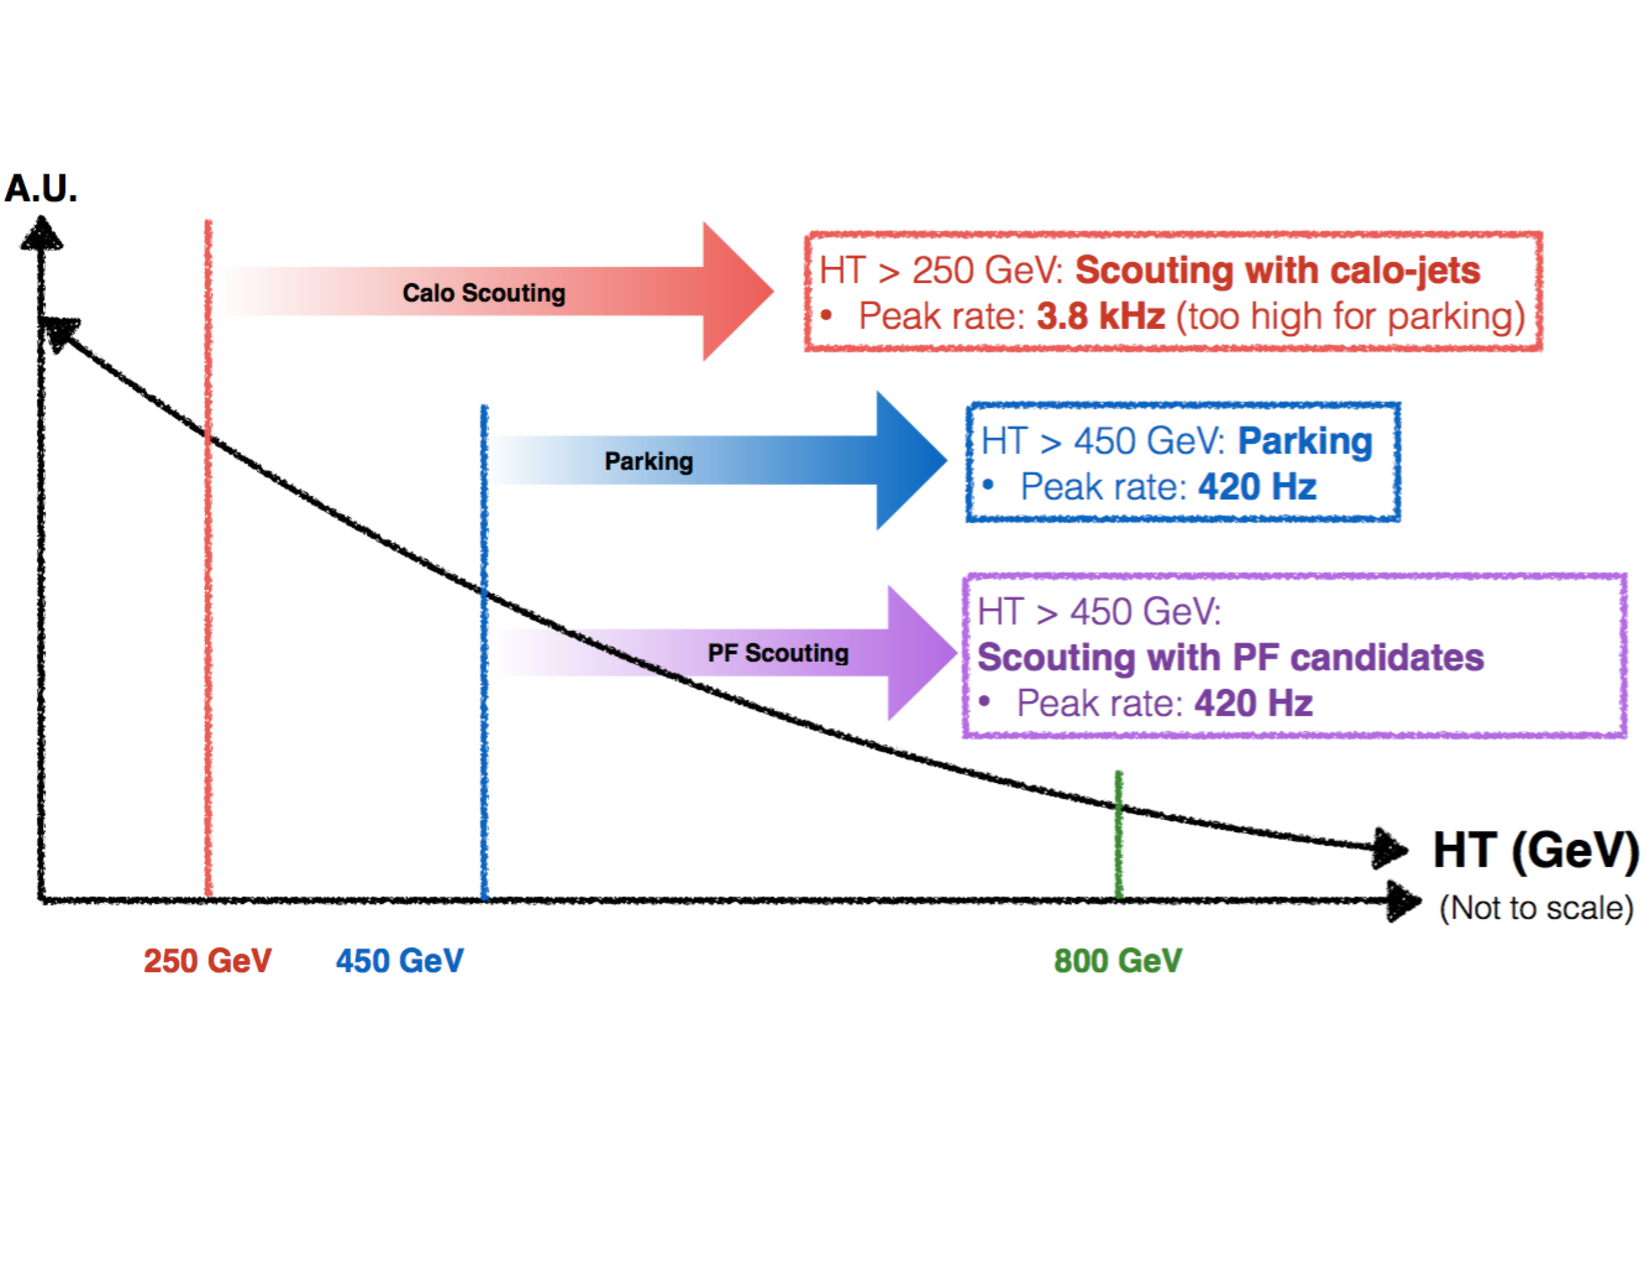
\includegraphics[width=.9\textwidth]{figs/cms/Scouting2015.pdf}\\
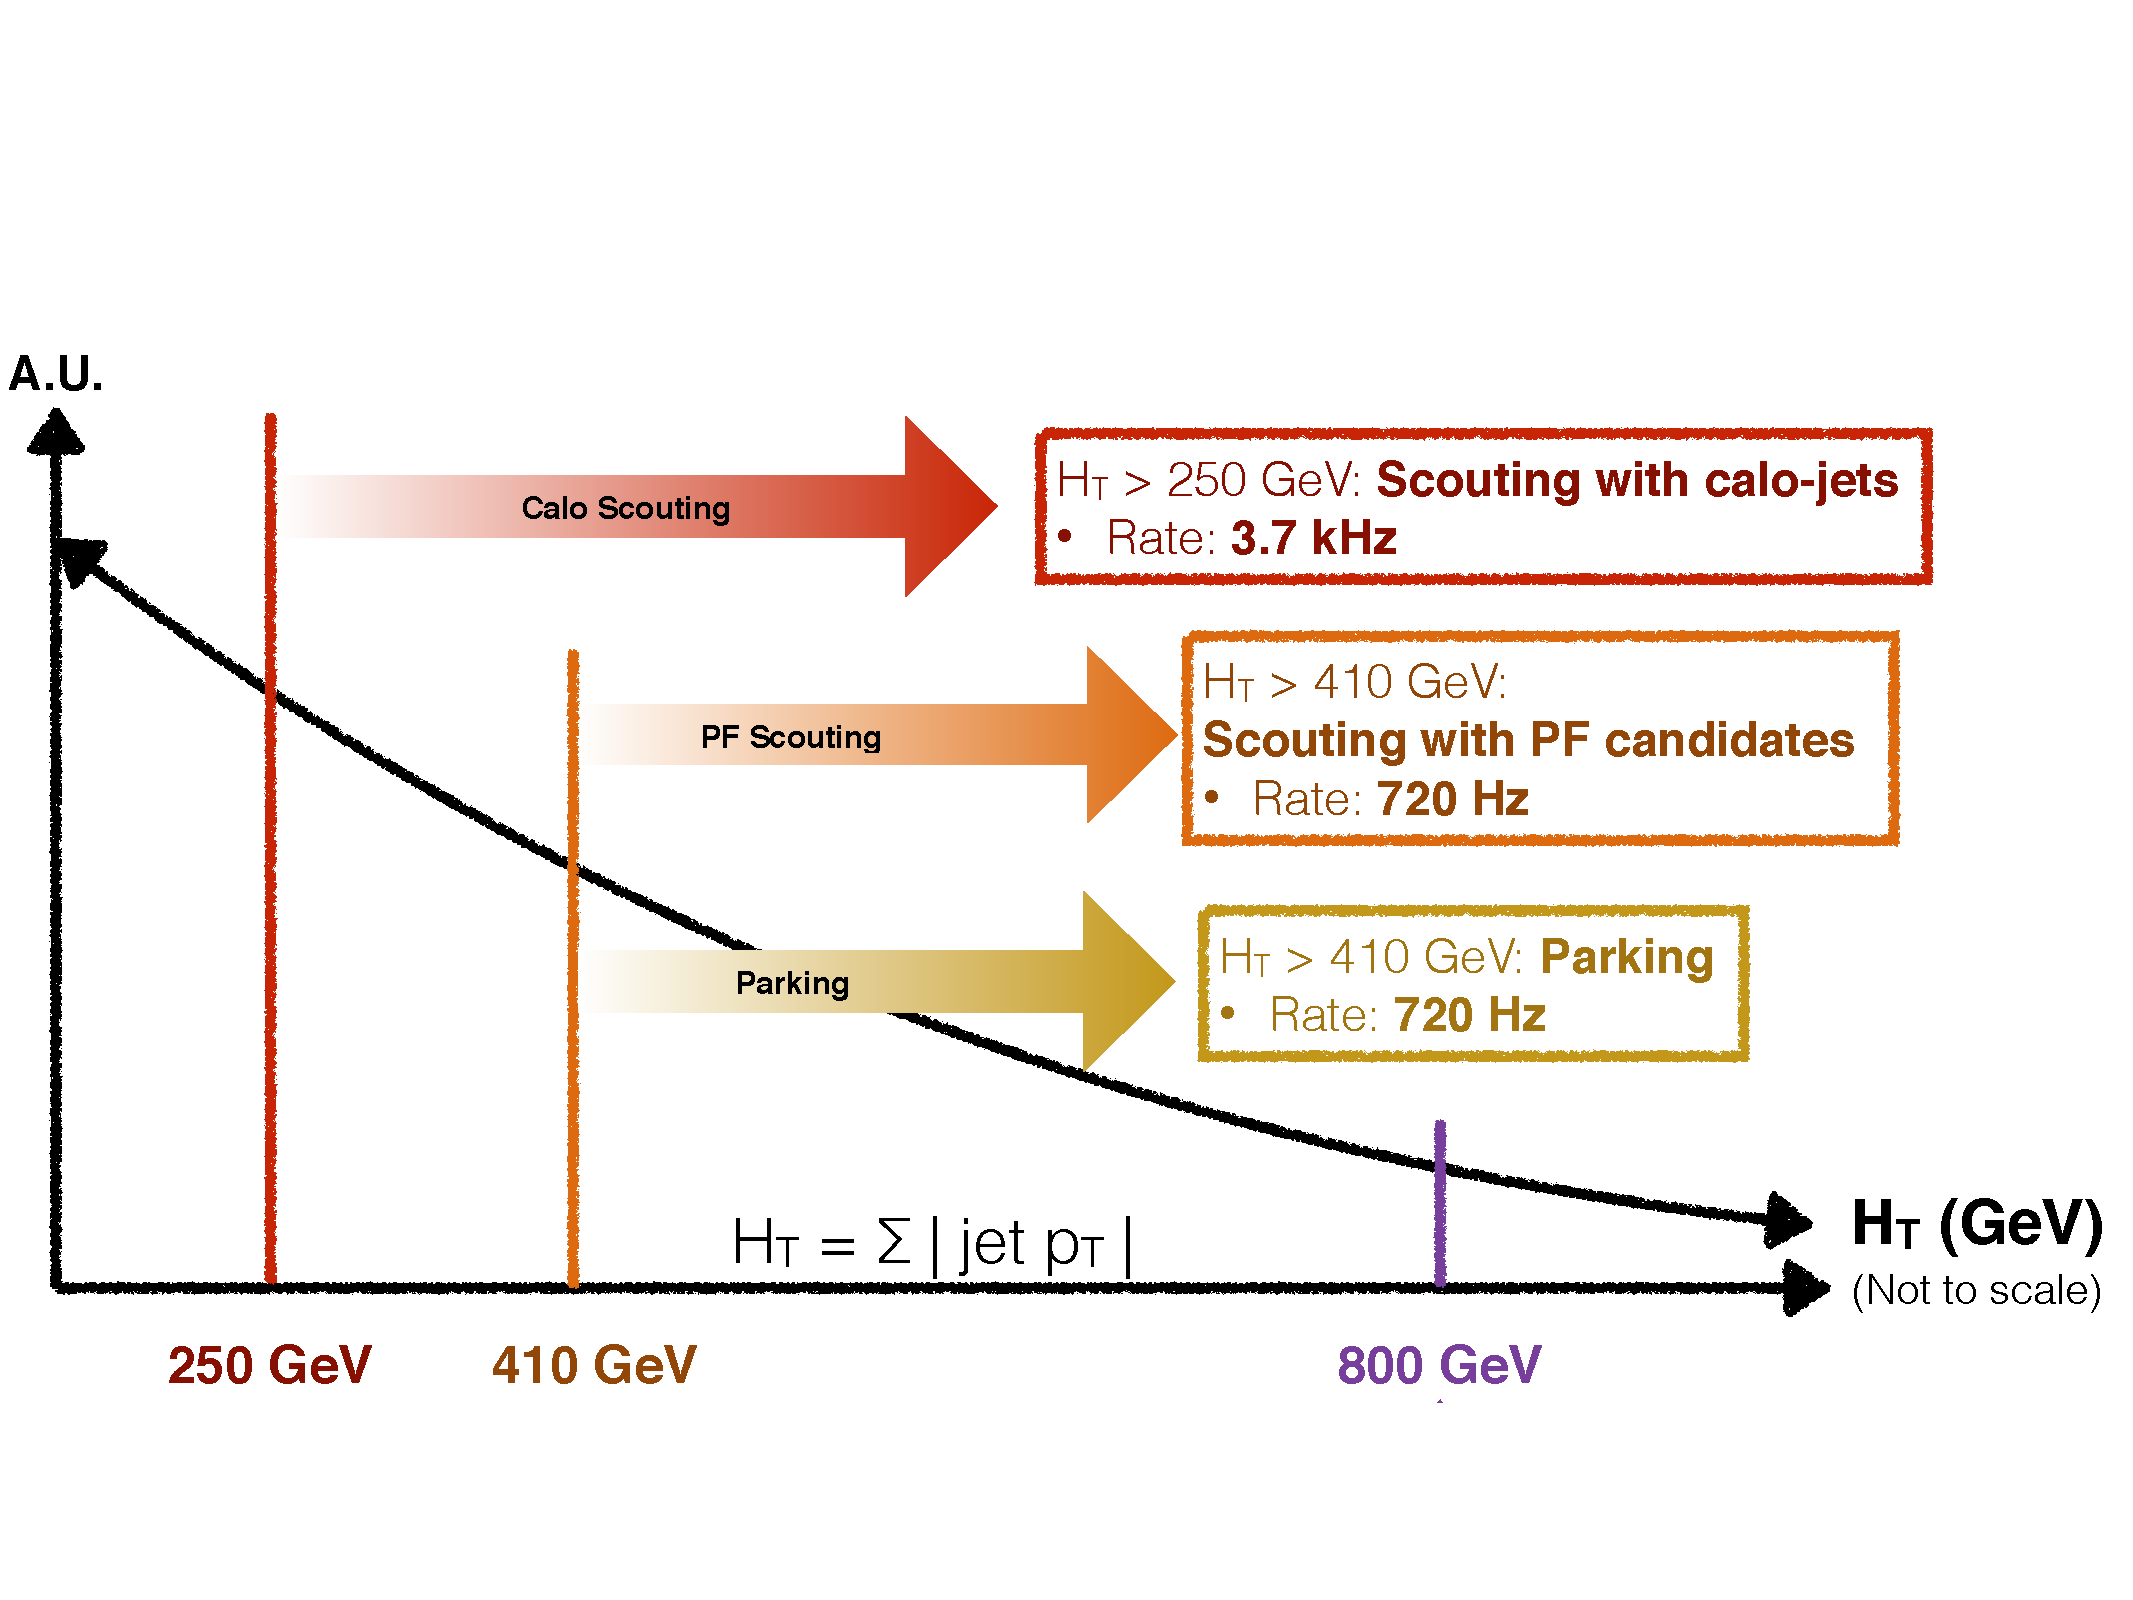
\includegraphics[width=.9\textwidth]{figs/cms/Scouting2016.pdf}
\caption{HLT $H_\mathrm{T}$ thresholds for Calo and PF scouting for
  2015 (top) and 2016 (bottom) data-taking runs. The
  rates for the 2015 (2016) are normalized to an instaneous luminosity
  of $7\times 10^{33}$ cm$^{-2}$ s$^{-1}$ ($10^{34}$ cm$^{-2}$
  s$^{-1}$). \label{fig:DataScouting}}
\end{figure}

\begin{figure}\centering
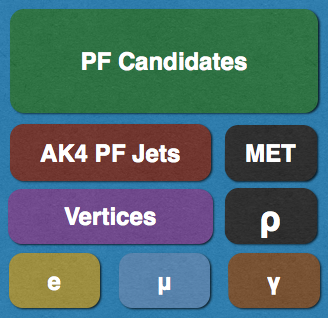
\includegraphics[width=.45\textwidth]{figs/cms/pfscoutingeventcontent.png}
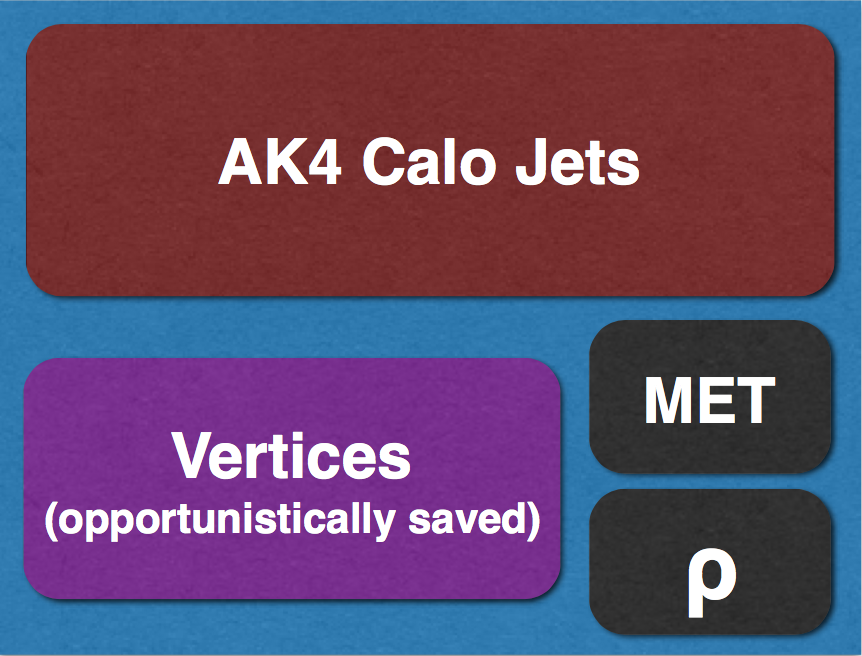
\includegraphics[width=.45\textwidth]{figs/cms/caloscoutingeventcontent.png}
\caption{The event content for PF scouting (left), which amounts to
  $\sim 10$\unit{kB}, and Calo scouting (right), which amounts to
  $\sim 1.5$\unit{kB}.\label{fig:DataScoutingContent}}
\end{figure}

\section{Alignment and Calibration}
\label{sec:alca}

Fast and efficient methods for the calibration and the alignment of
the detector are a key ingredient in exploiting the physics potential of
CMS. To this end, CMS has a powerful framework for alignment and
calibration, which is based on dedicated ``skims,'' or subsets of data samples, providing a highly
compact input for the various workflows computing the
calibration and alignment constants. 
%This includes a prompt calibration concept, which allows
%for a fast turnaround of the calibration process which is instrumental
%to ensure timely preparation of results for conferences and
%publications.
%The high level of complexity and the large number of detector channels
%reflect in an elaborated structure for the management and computation
%of the detector calibration and alignment. The present contribution
%reviews the workflows developed for this purpose focusing on a few
%selected examples. 

Most of the alignment and calibration workflows are fed with dedicated
data samples, called AlCaReco, optimized both in terms of event
selection and event content. Depending on the needs of the specific
workflow, these samples can be selected offline, while performing the
reconstruction, or directly online, at the HLT level. 
%The great
%flexibility of the HLT, which runs offline-quality software on a farm of commercial processors, is a key asset for this
%online selection since it guarantees an adequate rate of events that
%would not be selected by the standard trigger paths meant for physics
%analysis.

An example of an online calibration stream is the one selecting events
containing $\pi^0$ and $\eta$ candidates detected in the ECAL and used
for the intercalibration of the PbWO$_4$ scintillating
crystals~\cite{Chatrchyan:2013dga}. The calibration performance
depends on the number of selected $\pi^0$ candidates per crystal and
on the signal-to-background ratio. The candidate diphoton decays are
selected at the HLT level from events passing single-$e/\Pgg$ and
single-jet L1 triggers. After selection, only information about a
limited region of ECAL (energy deposits in 20 to 40 individual
crystals) near the $\pi^0$ candidates is stored for the actual
calibration. This allows to sustain a high rate of calibration events
(1 to 10 kHz) whilst saving bandwidth and CPU time.


Detector conditions that change on a short time scale require a special
calibration workflow designed to allow updates with very short
latency. To meet this need, the organization of data streams is as follows:
\begin{itemize}
\item express processing: reconstruction of a limited selection of
  data in order to give quick feedback about the detector status and
  physics performance and to provide data for calibration
  workflows. The results of the express reconstruction for a given run
  are usually available one or two hours after the raw data are
  collected;
\item bulk processing: reconstruction of the main data stream for
  physics analysis. This step, called prompt reconstruction, is
  delayed by 48 hours to allow for the computation and usage of 
  new calibration constants relating to fast-changing conditions. The output is divided in
  several Primary Datasets (PD) on the basis of the HLT paths that select the events;
\item calibration streams: streams of events selected at the HLT level
  and processed at Tier-0 for calibration purposes.
\end{itemize}

During Run 1 normal operation, about $300-400$\unit{Hz} of data 
were processed in the bulk processing, while about $30-40$\unit{Hz} was allocated for express
processing in order to guarantee a fast reconstruction. A selection of
data from the express and calibration streams is used
to compute the updated conditions for a given run while the bulk of
the data is buffered on disk. The calibration workflows run on a
dedicated farm at CERN called the CMS Analysis Facility (CAF). In this
way the prompt reconstruction can profit from the updated constants,
reducing the need for offline reprocessing of the data. This workflow
is called the \emph{prompt calibration loop} and is illustrated schematically
in Fig.~\ref{fig:AlCa}. The conditions currently updated through this kind of
workflow are:
\begin{itemize}
\item measurement of the beam-line parameters;
\item monitoring and masking of problematic channels of the silicon strip tracker to respond to
HV trips or noise;
\item transparency corrections based on the laser monitoring system for the PbWO$_4$ crystals of the ECAL
  calorimeter.
\end{itemize}
The delayed prompt reconstruction is also exploited to
monitor possible movements of large structures of the silicon tracker,
mainly due to thermal stress, and problematic channels in the
electromagnetic and hadronic calorimeters allowing for quick reaction
time in case of ``hot'' regions identified in the express
reconstruction.

\begin{figure}\centering
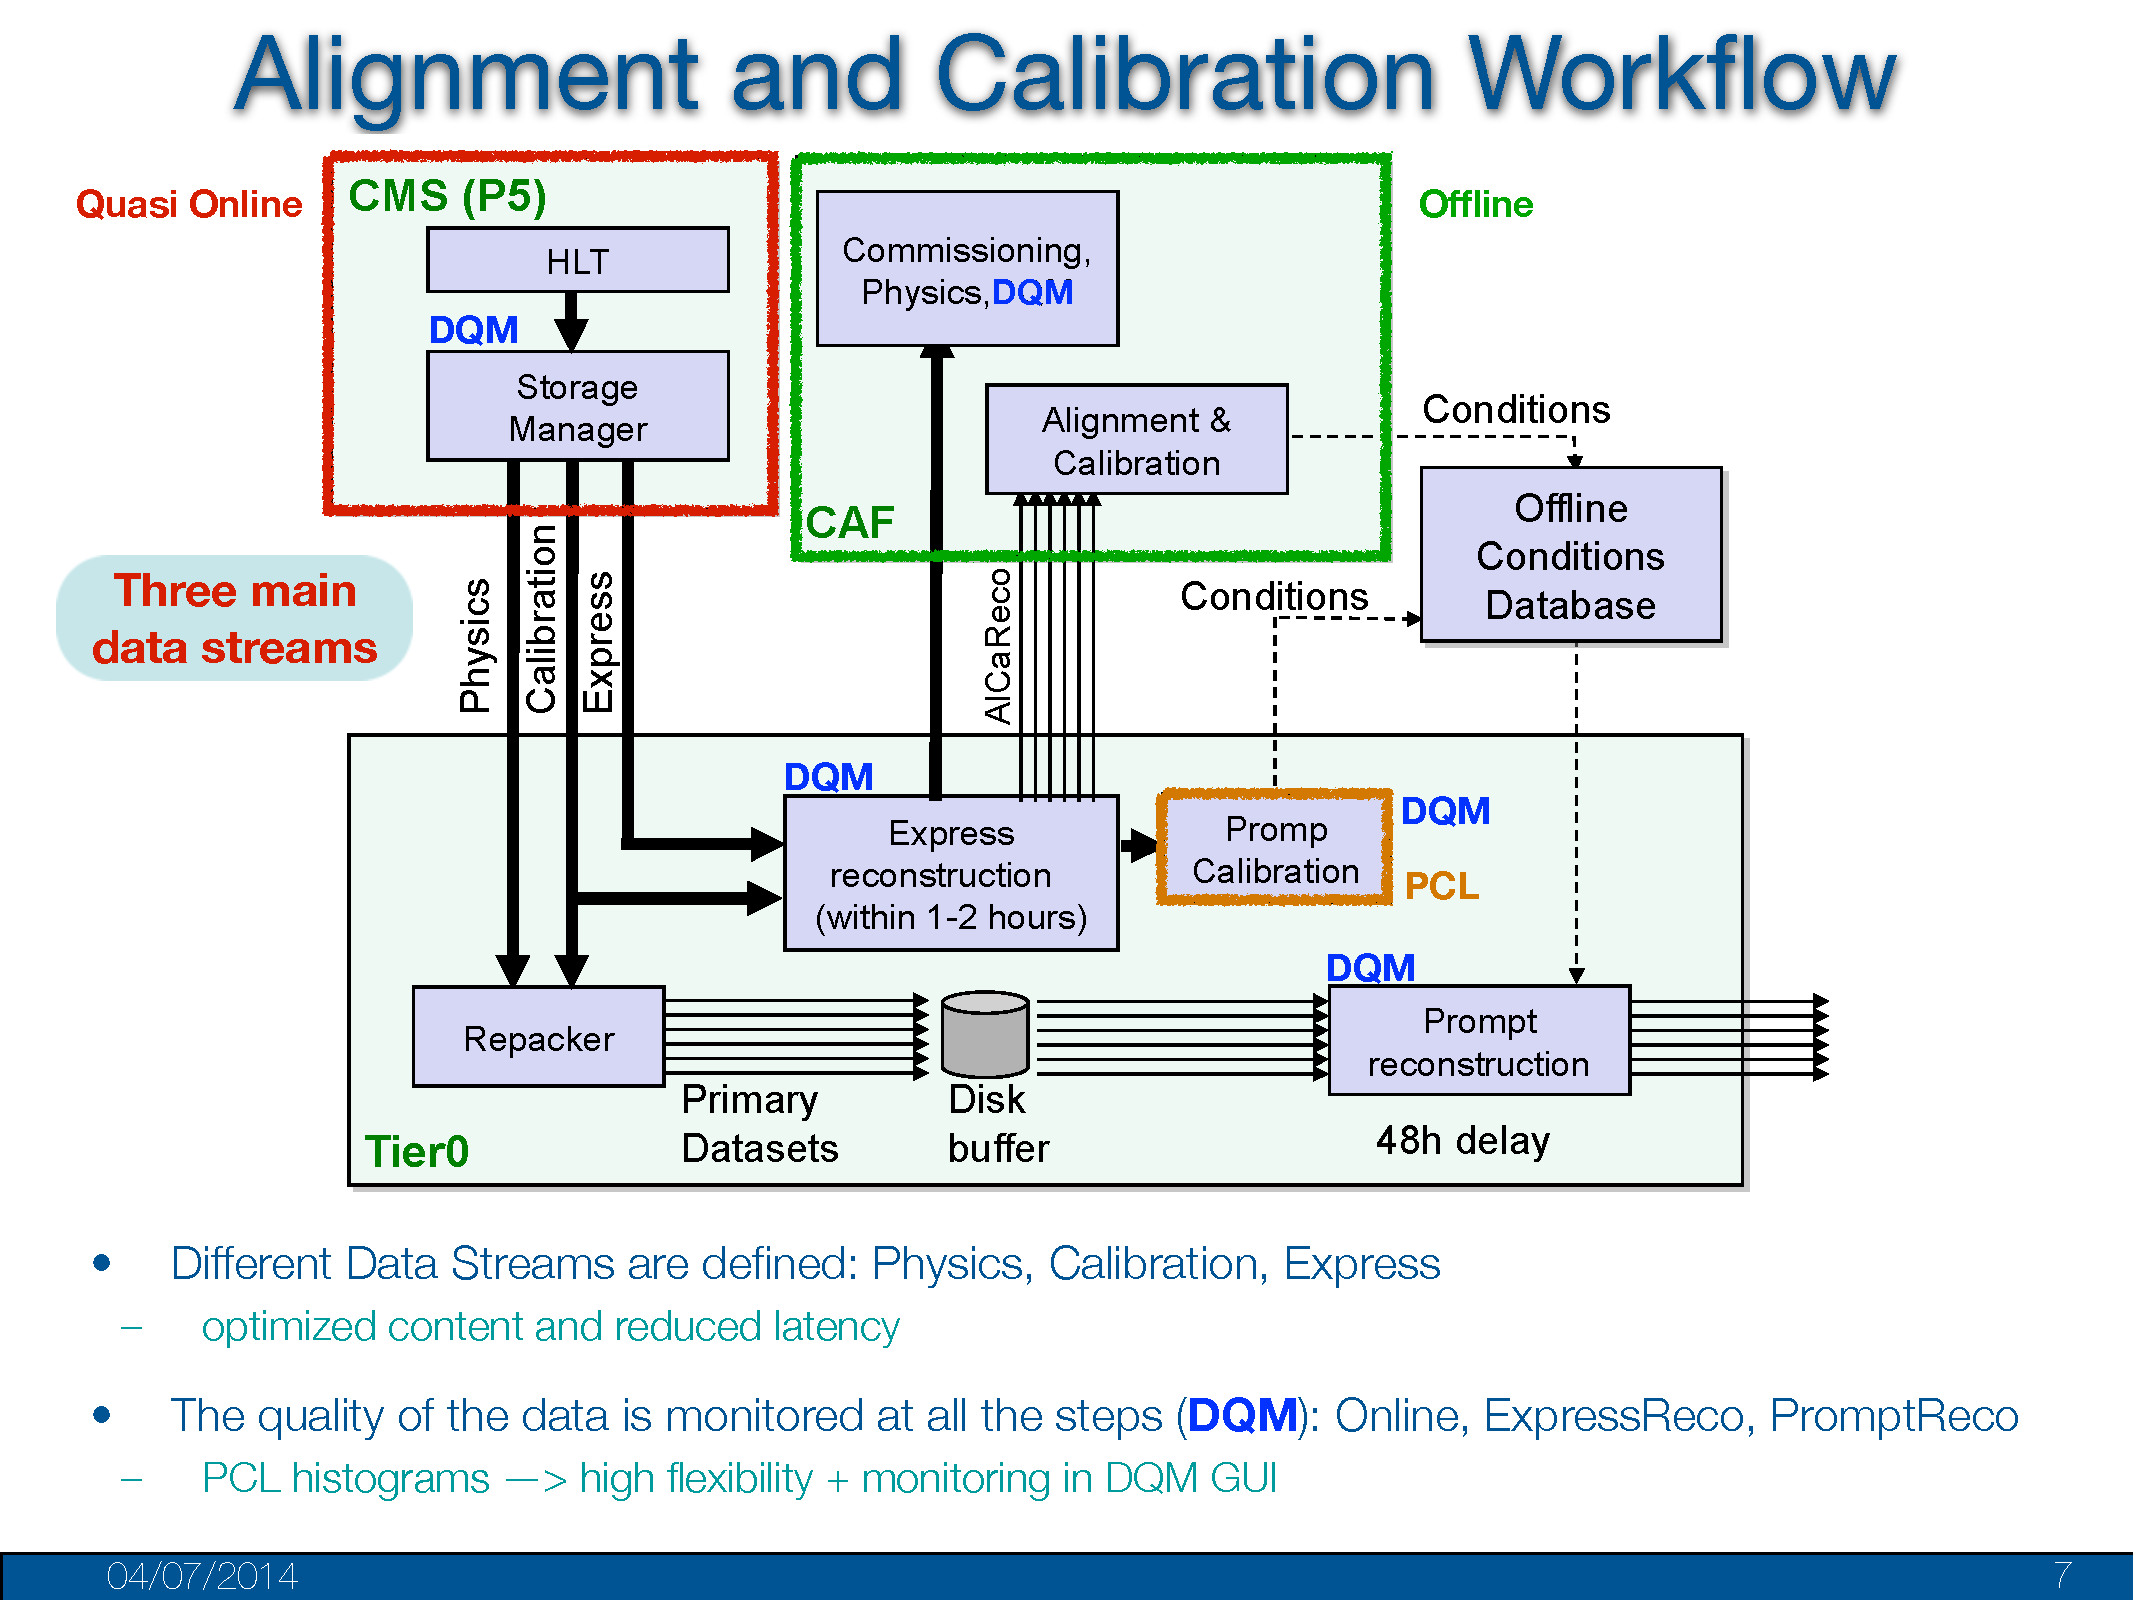
\includegraphics[width=.9\textwidth,clip=true,viewport=0 180 900 700]{figs/cms/AlCa.pdf}
\caption{Alignment and calibration data-processing flow.\label{fig:AlCa}}
\end{figure}

In order to reach the ultimate accuracy, more sophisticated
alignment and calibration workflows are run offline. No time
constraints are present in this case and the full treatment of the
detector’s alignment and calibration inter-dependencies can be
studied and taken into account. The full data sample is exploited to
provide the final set of conditions which are then used in the
reprocessing of the data. In normal conditions the full dataset is
reprocessed once per year. Some important offline workflows are as follows:
\begin{itemize}
\item energy calibration of the ECAL response (single channel and overall energy scale calibration);
\item measurement and correctionion of the tracker orientation with respect to the magnetic field;
\item tracker module alignment.
\end{itemize}

A third class of calibration workflows, the quasi-online calibration,
is meant to update conditions at HLT for data taking. %The measurement
%of the beam-line parameters falls in this category as well. 
For some very stable corrections that do not need to be validated, such as the measurement of beam-line
parmaters, an application running in the Data Quality Monitoring (DQM)
framework~\cite{DeGuio:2014taa} automatically derives and stores conditions in a database which is
then accessed at the HLT during the online event
reconstruction. This feedback from the DQM to the HLT happens with a
time granularity of 2 minutes (5 luminosity sections).
For other corrections that do need to be validated, such as the ECAL transparency
corrections, a validation workflow is run, involving ECAL experts who
derive, carefully check, and upload the corrections to the database on
a weekly basis during data taking.


\subsection{ECAL Laser Monitoring}

The crystals have to withstand the damage to the crystal
lattice caused by radiation expected throughout the duration of LHC operation. The
expected integrated ionizing dose in the ECAL is up to $4$ \unit{kGy} in the
barrel and $200$ \unit{kGy} at $\abs{\eta} = 3$ after $10$ years of LHC operation
corresponding to an integrated luminosity of $500$ \fbinv~\cite{CMSECALTDR}. The
expected hadron fluence varies between about $10^{13}$ cm$^{-2}$ in the barrel
and $10^{14}$ cm$^{-2}$ at $\abs{\eta} = 3$. The main observable effect of the radiation
is a wavelength-dependent loss of crystal transparency due to the
formation of color centers, but without changes to the scintillation
mechanism~\cite{Adzic:2009aa}. In order to measure and correct for
response change during LHC operation, the ECAL is equipped with a
light monitoring (LM) system~\cite{Anfreville:2007zz,Zhang:2005ip}. 

The evolution of the ECAL response to the laser light (440 \unit{nm} in 2011 and 447 \unit{nm} from 2012 onwards) from 2011
through 2016 is shown in Fig.~\ref{fig:ECALLaserHistory}, as a function of time~\cite{CMS-DP-2016-031}. 
%An average value is shown for each of six pseudorapidity ranges. The data are normalized to the
%measurements at the start of 2011. The corresponding instantaneous
%luminosity is also shown. 
The response drops during periods of LHC operation, and recovers
during shutdown periods (or periods of low-luminosity data-taking). These
observations correspond to changes in crystal
transparency~\cite{Adzic:2009aa} and are used to correct the physics
data. The response change observed in the ECAL channels is up to 6\% in the
barrel and it reaches up to 30\% at $\abs{\eta} \sim 2.5$, the limit
of the tracker acceptance. The response change is up to 70\% in the
region closest to the beam pipe. 

%A second effect of the
%radiation is that the VPT response decreases with accumulated
%photocathode charge to a plateau [17]. Radiation does not affect the
%gain of the APDs but in large doses induces dark currents which cause
%small reductions in the bias voltage at the APDs if not compensated
%for. 

\begin{figure}\centering
%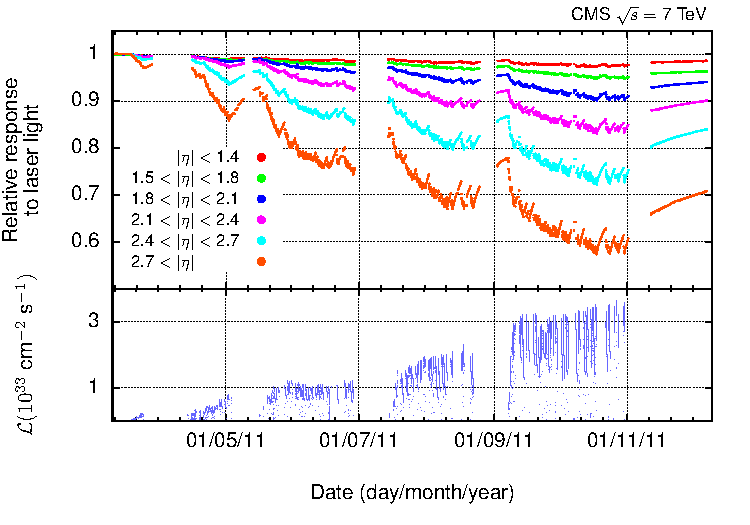
\includegraphics[width=.9\textwidth]{figs/cms/histories_2011_v2.pdf}
\includegraphics[width=.9\textwidth]{figs/cms/histories_2016.pdf}
\caption{Relative response to laser light from 2011 to 2016, normalized to
  data at the start of 2011. An average is shown for each
  pseudorapidity range. The bottom plot shows the corresponding
  instantaneous luminosity. After each LHC technical stop, a
  recovery of crystal transparency is observed.\label{fig:ECALLaserHistory}}
\end{figure}

The ECAL light monitoring system is used to determine corrections,
denoted $S(t)$, to response changes in the ECAL. The
laser light is injected through optical fibers in each crystal. The spectral
composition and the path for the collection of laser light at the
photodetector are different from those for scintillation light. A
conversion factor is required to relate the changes in the ECAL
response to laser light to the changes in the scintillation
signal. The relationship is described by a power law~\cite{CMSECALTDR}:
\begin{equation}
\frac{S(t)}{S_0} = \left(\frac{R(t)}{R_0}\right)^{\alpha}~,
\end{equation}
where $S(t)$ is the channel response to scintillation light at a particular time $t$, $S_0$ is the initial
response, and $R(t)$ and $R_0$ are the corresponding response to laser
light. The exponent $\alpha$ is independent of the loss for small
transparency losses and was measured in test beams to be $1.52$ and
$1.0$ for crystals from the two different
producers~\cite{VanLysebetten:787485,Adzic:2006za,Ghezzi:934066}.

Different forms of these laser corrections, differing in time and
spatial granularity, are utilized at different
times in the data processing: online at the HLT, during the prompt
reconstruction, and during offline reprocessing of the data. At HLT,
the laser corrections are updated once-per-week and are applied to 11
different $\eta$ rings in each endcap and 17 different $\eta$ rings in
the barrel (the corrections are averaged over each ring). For the prompt reconstruction and the offline
reprocessing, the laser corrections are updated every 40 minutes
and are applied crystal-by-crystal.

The validation of the HLT laser corrections uses a custom workflow which
re-runs the HLT reconstruction on recently collected data with two versions of
laser corrections: the version currently online (and now out-of-date)
and the version to be validated (and up-to-date). An example of a
succesfully validated HLT laser correction for a particular week of
data-taking in 2015 is shown in Fig.~\ref{fig:ECALHLT}. Unlike the
outdated laser corrections (shown in blue), the updated
laser corrections (shown in black) correct the energy response and
improve the energy resolution for both the endcaps and the barrel.

\begin{figure}\centering
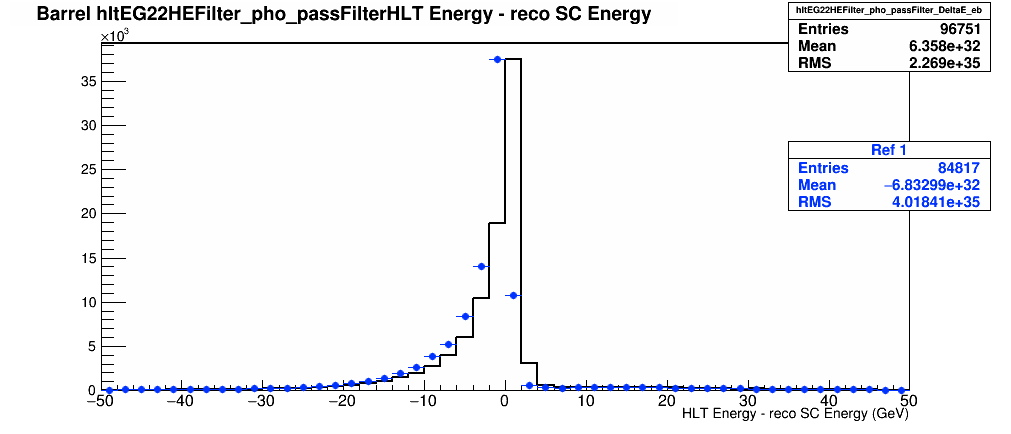
\includegraphics[width=.9\textwidth]{figs/cms/Week42_transpCorr_EB_overlay_IntermediateBlack_oldBlue.png}\\
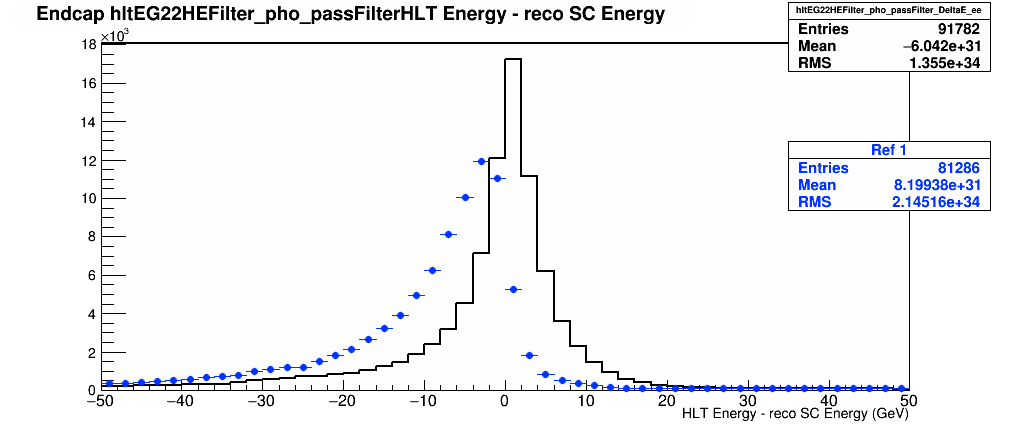
\includegraphics[width=.9\textwidth]{figs/cms/Week41_transpCorr_EE_overlay_newBlack_oldBlue.png}
\caption{The top (bottom) plot shows the difference between the supercluster energy
  reconstructed at HLT and a reference energy for the ECAL barrel (endcaps) for a particular
  week of data-taking in 2015. The blue data points show the
  difference using the week-old laser corrections, while the solid black histogram shows the reconstructed energy with the
  updated laser correction undergoing validation.\label{fig:ECALHLT}}
\end{figure}
%https://twiki.cern.ch/twiki/bin/viewauth/CMS/EGammaHLT2015LaserCorrValWeeklyReport

The $\Pgh$ meson data are used to validate the laser corrections for prompt reconstruction. The events are
selected online by a dedicated calibration trigger and recorded with
reduced event content. A fit is carried out on the invariant mass distribution of the photon
pairs in the mass range of the $\Pgh$ meson. The fit comprises a
polynomial function to describe the background and a Gaussian
distribution to describe the resonance peak. Fig.~\ref{fig:etaEB}
shows an example of the $\Pgh$-meson peak with the fit superimposed,
and the relative value of the fitted $\Pgh$ mass versus time in EB for
a period of 60 hours. The plot shows the data before (red points) and
after (green points) the laser corrections applied. A number of
measurements are possible for each LHC fill, owing to the high
rate for recording $\Pgh$ events. This permits short-term changes in
the ECAL response to be verified before the prompt reconstruction
takes place.

\begin{figure}[bht]
\begin{center}
 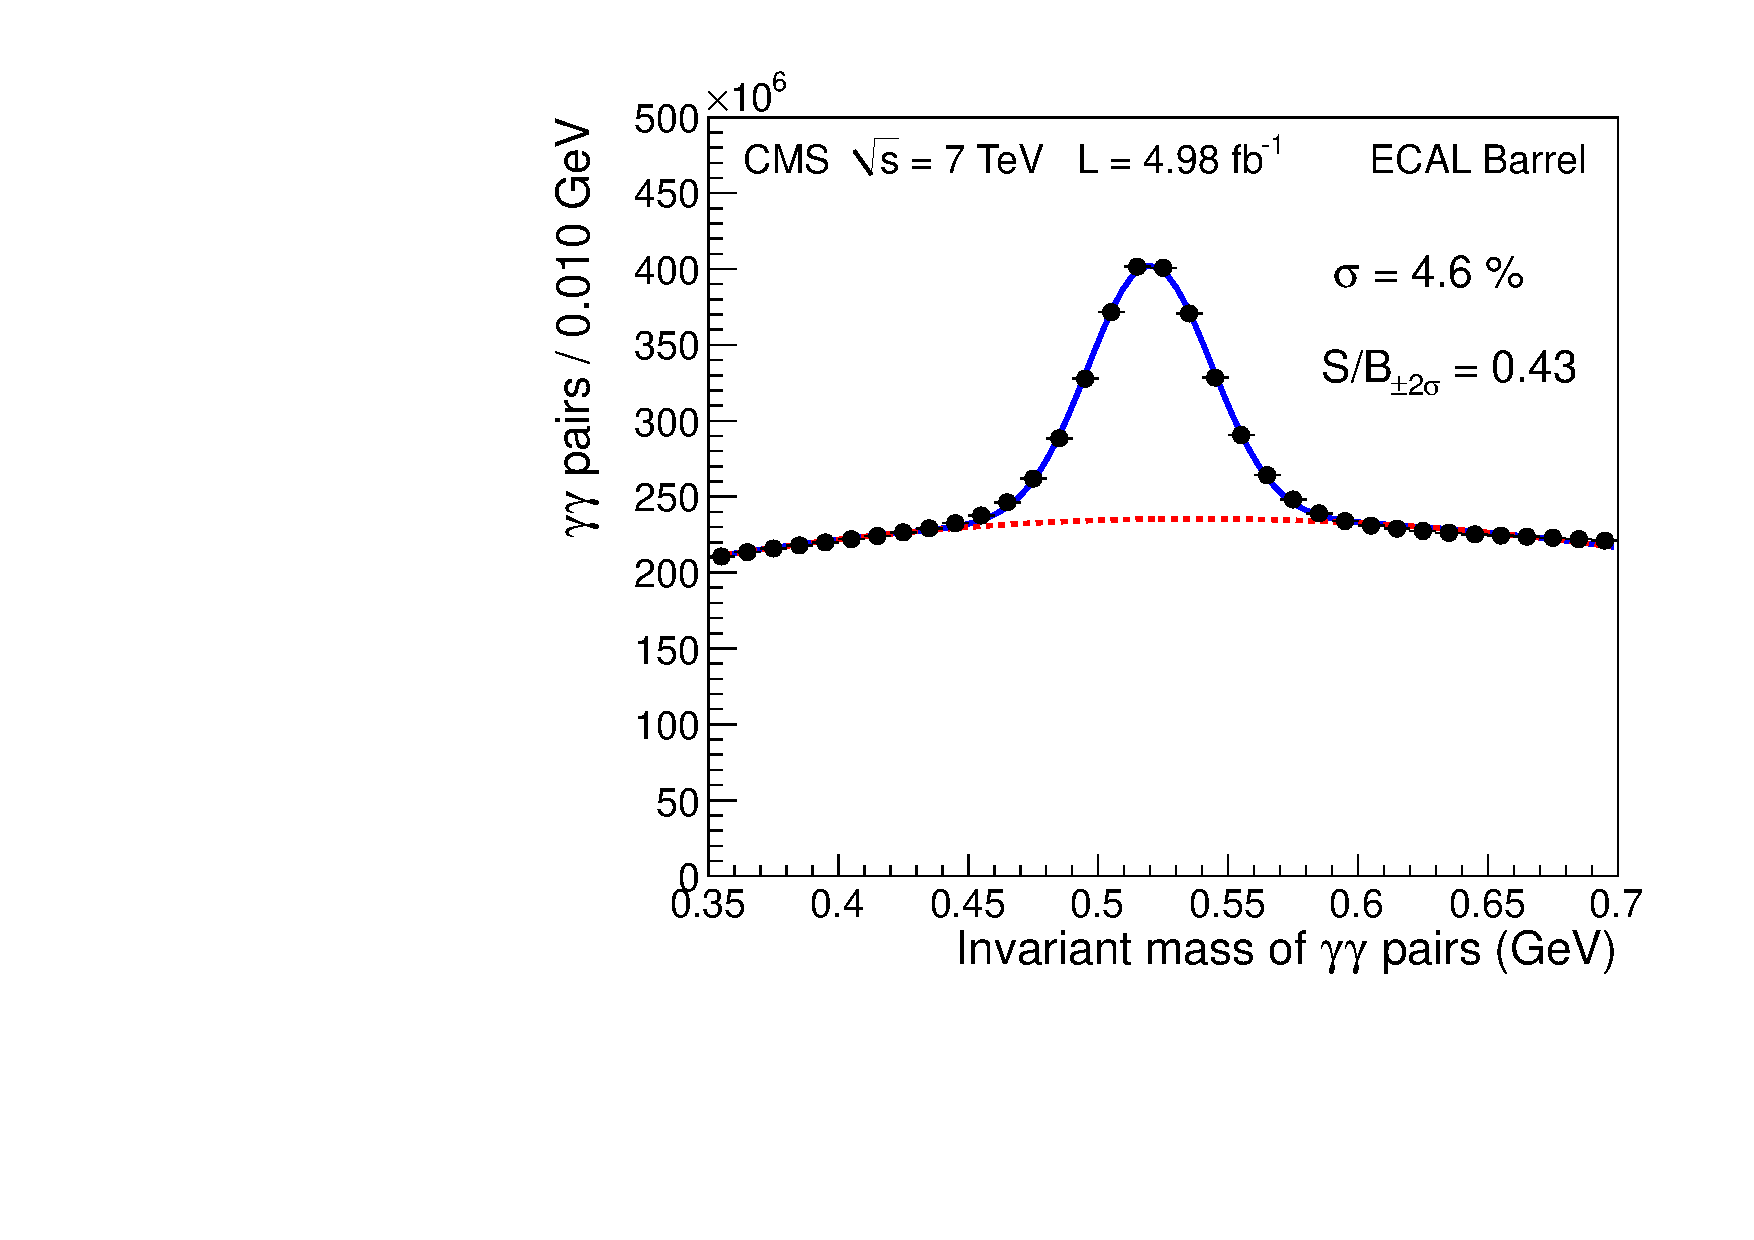
\includegraphics[width=0.40\linewidth,height=5.6cm]{figs/cms/eta_peak.pdf}
 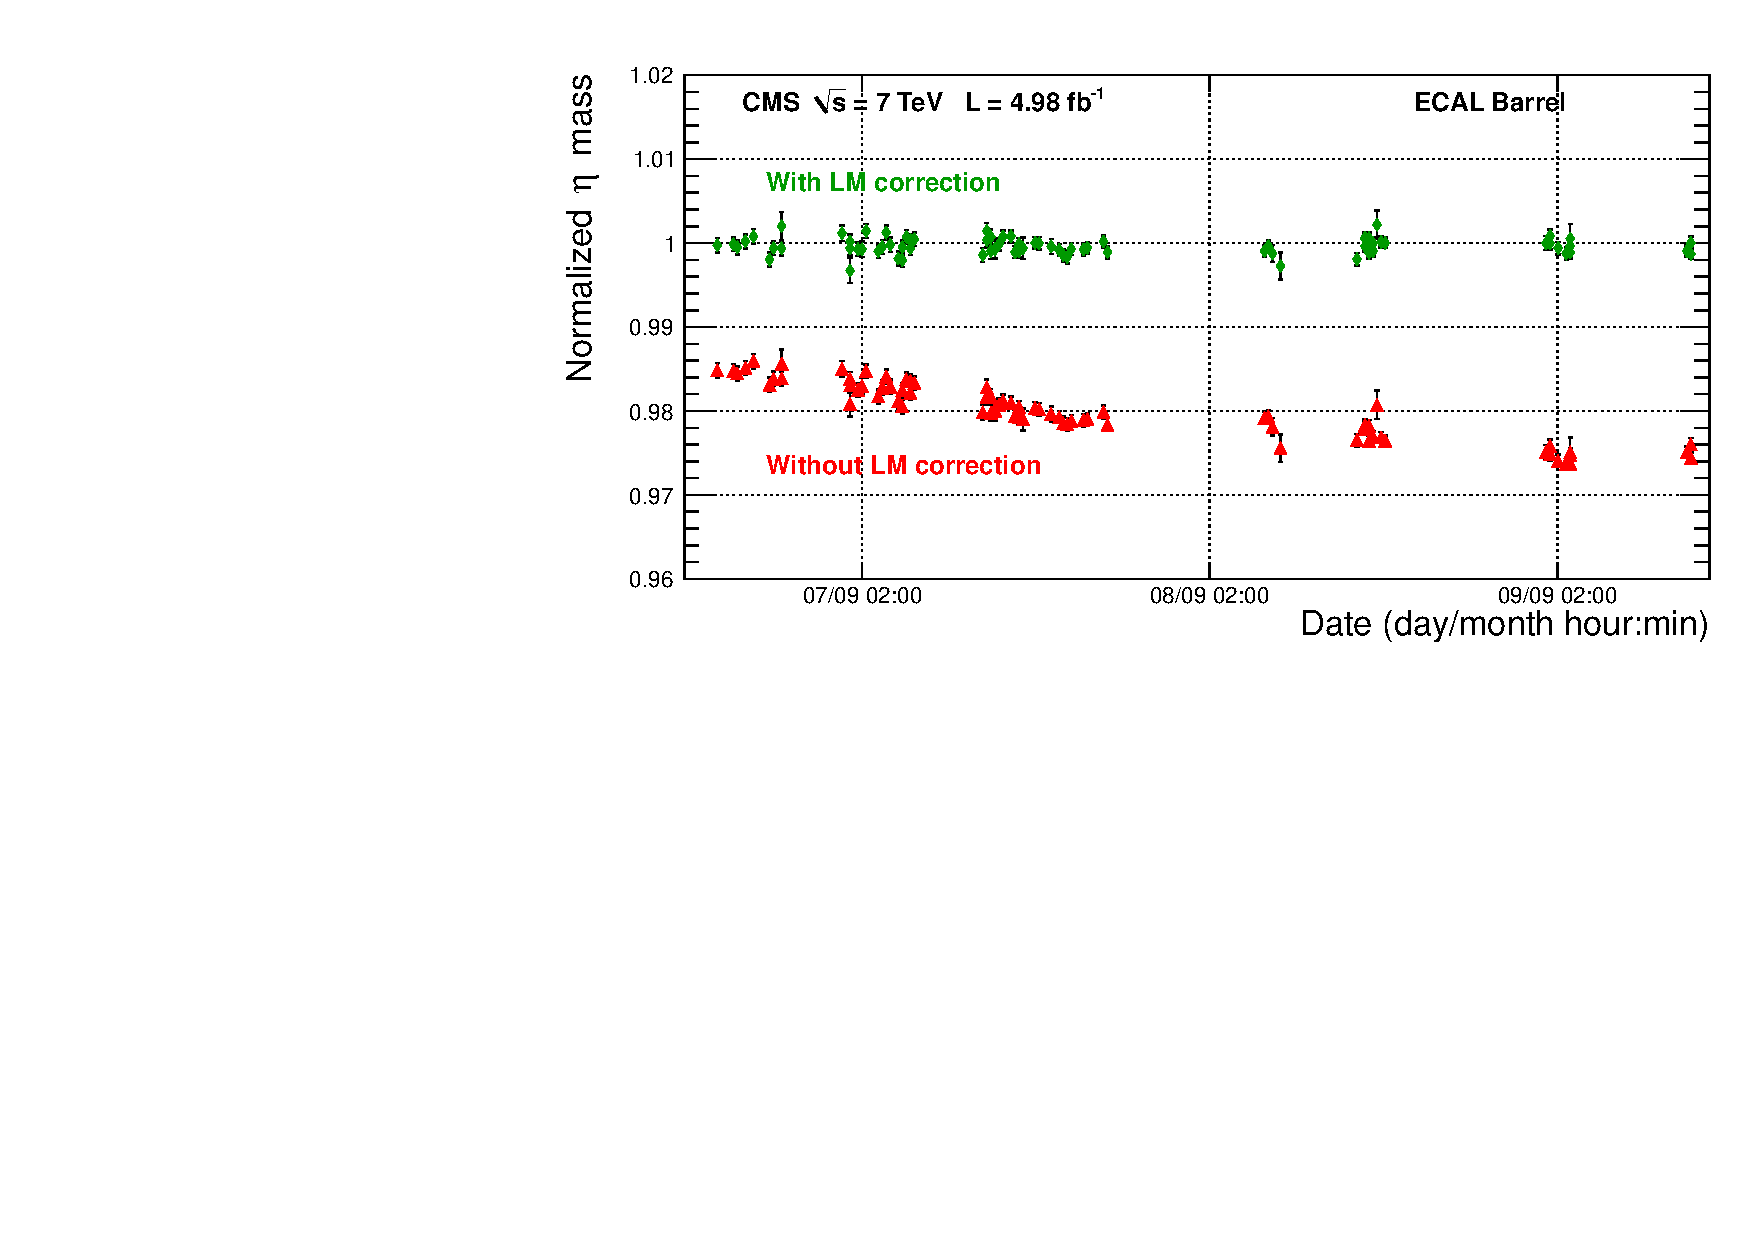
\includegraphics[width=0.59\linewidth,height=5.6cm]{figs/cms/eta_zoom.pdf}
\end{center}
\caption{\label{fig:etaEB}
Left: An example of the $\Pgh$-meson peak reconstructed from the invariant
mass of photon pairs in the barrel, with the result of the fit with a Gaussian
distribution (continuous line) and a polynomial function (dotted line);
Right: Stability of the $\Pgh\to\Pgg\Pgg$ mass measurement in the barrel as a
function of time, over a period of 60 hours, for data recorded in
September 2011. The plot shows the data with (green points) and
without (red points) laser corrections applied.}
\end{figure}

Finally, isolated electrons from $\PW$-boson decays are used to provide an energy
scale to validate the laser corrections over periods of days to
weeks. The event selection is described
in~\cite{EGM-10-004,Khachatryan:2010xn}.
The ratio of the electron energy, $E$, measured in the ECAL, to the
electron momentum, $p$, measured in the tracker, is computed in each
event, and a reference $E/p$ distribution is obtained from the entire
data set after applying laser corrections. The width of the $E/p$
reference distribution is dominated by the energy and momentum
resolution and is not biased by residual imperfections in the laser
corrections. This reference distribution is then scaled to fit
$E/p$ distributions obtained by dividing the same data in groups of
12000 consecutive events. The scale factors provide a measure of the
relative response and are shown in Fig.~\ref{fig:wenuEB} for 2011, as
a function of time. The data are shown before (red points) and after
(green points) laser corrections to the ECAL channel response are
applied. The magnitude of the average correction for each point is
indicated by the continuous blue line. A stable response to
electromagnetic showers is achieved throughout 2011 with an RMS of
0.12\% in the barrel and 0.35\% in the endcaps. This method does not require a
knowledge of the absolute calibration of both the energy and the
momentum.

\begin{figure}
\begin{center}
\begin{tabular}{cc}
 \hspace{-0.5cm}
 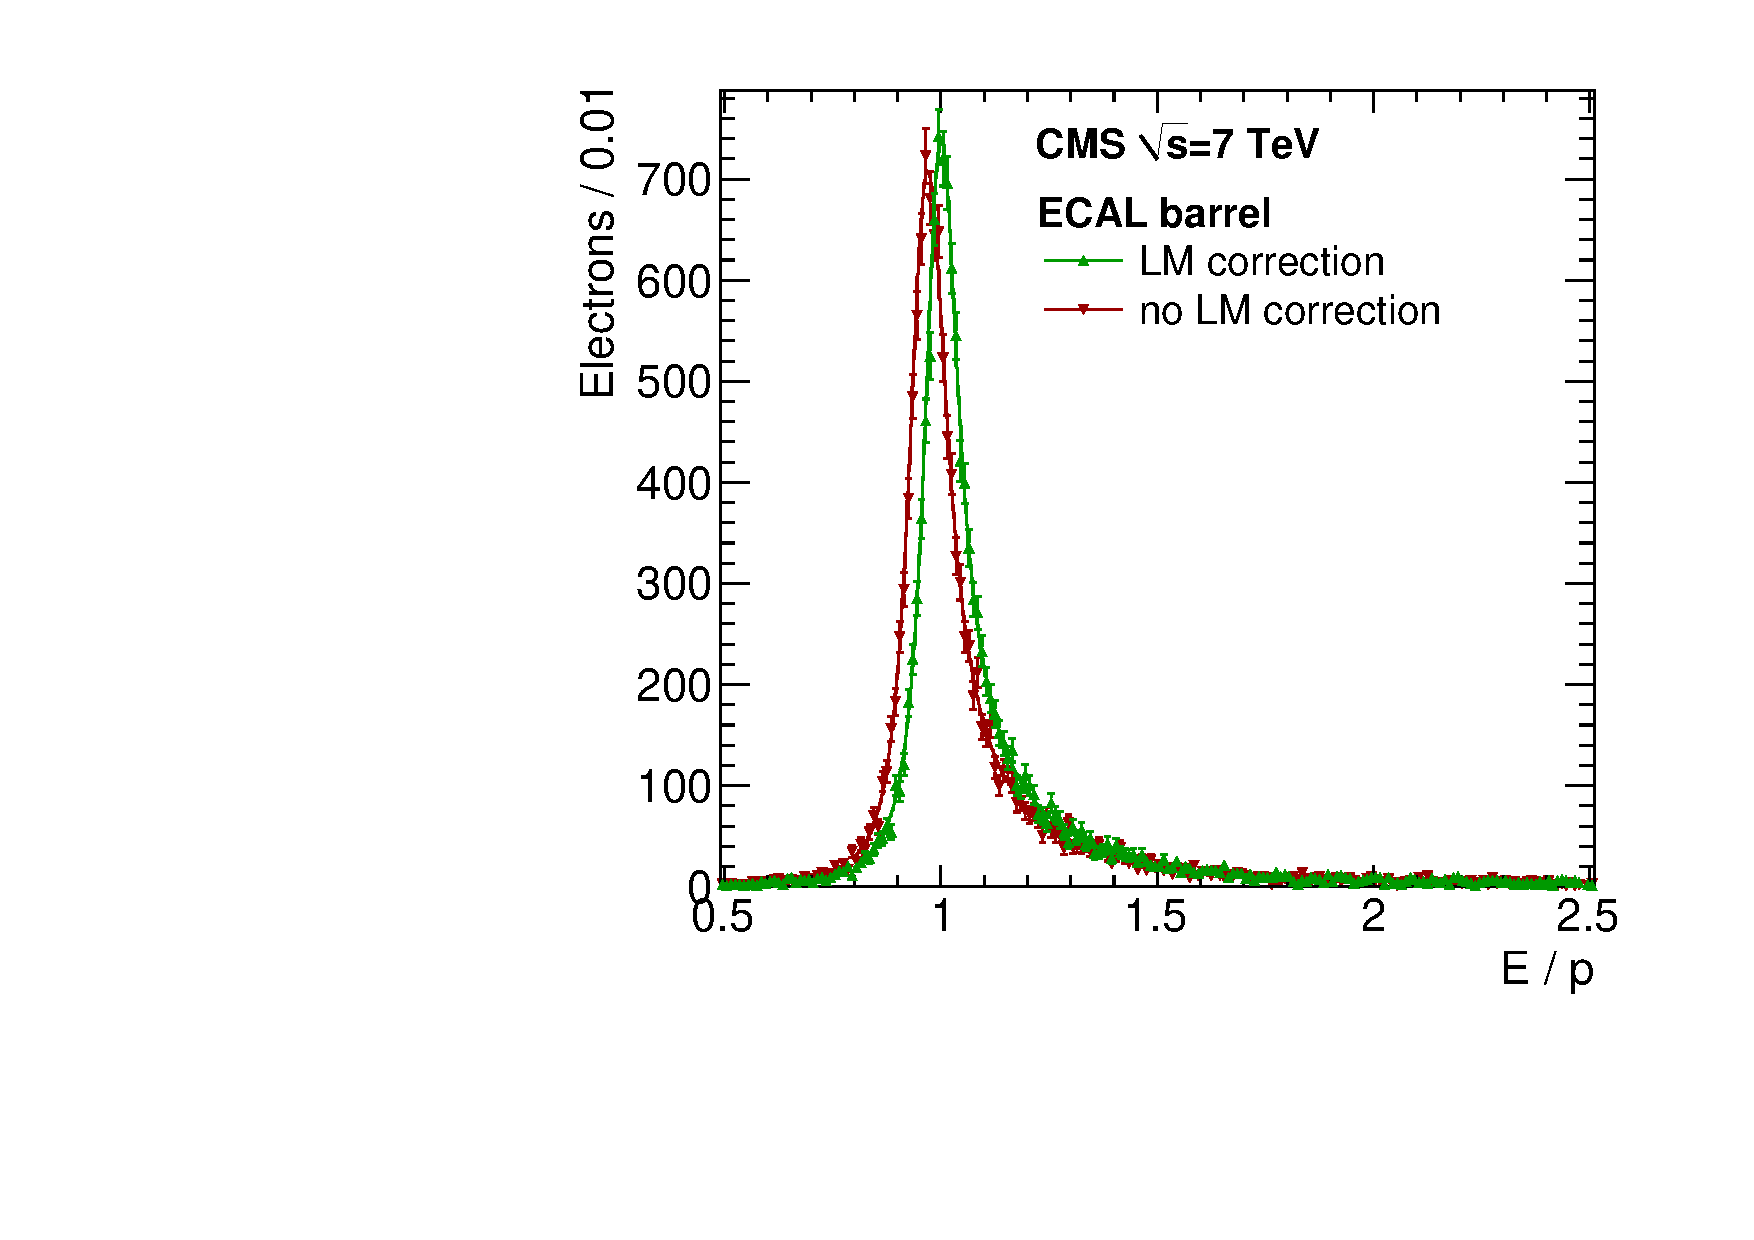
\includegraphics[width=0.40\linewidth]{figs/cms/EoP_TypicalFit_EB.pdf} &
 \hspace{-1cm}
 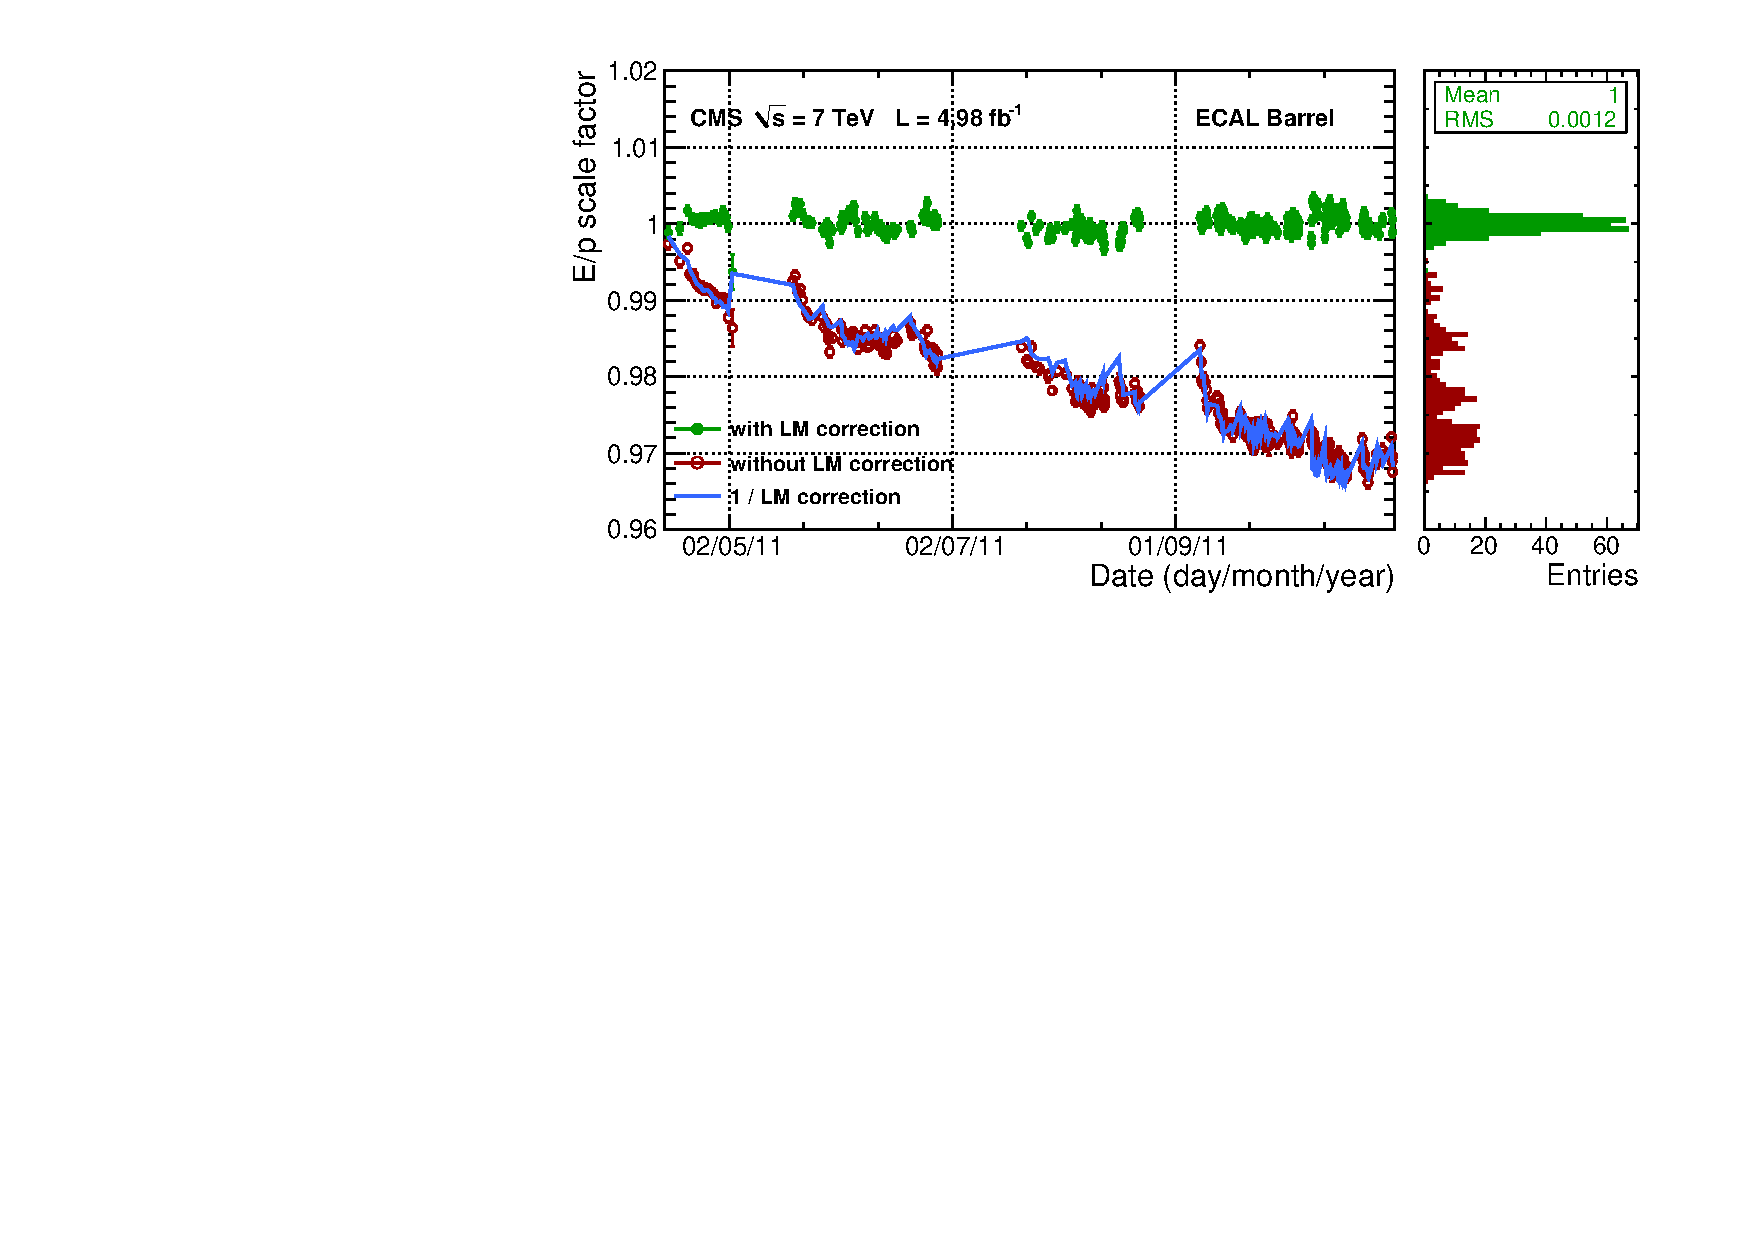
\includegraphics[width=0.69\linewidth]{figs/cms/EsuPhistoryEB.pdf} \\
 \hspace{-0.5cm}
 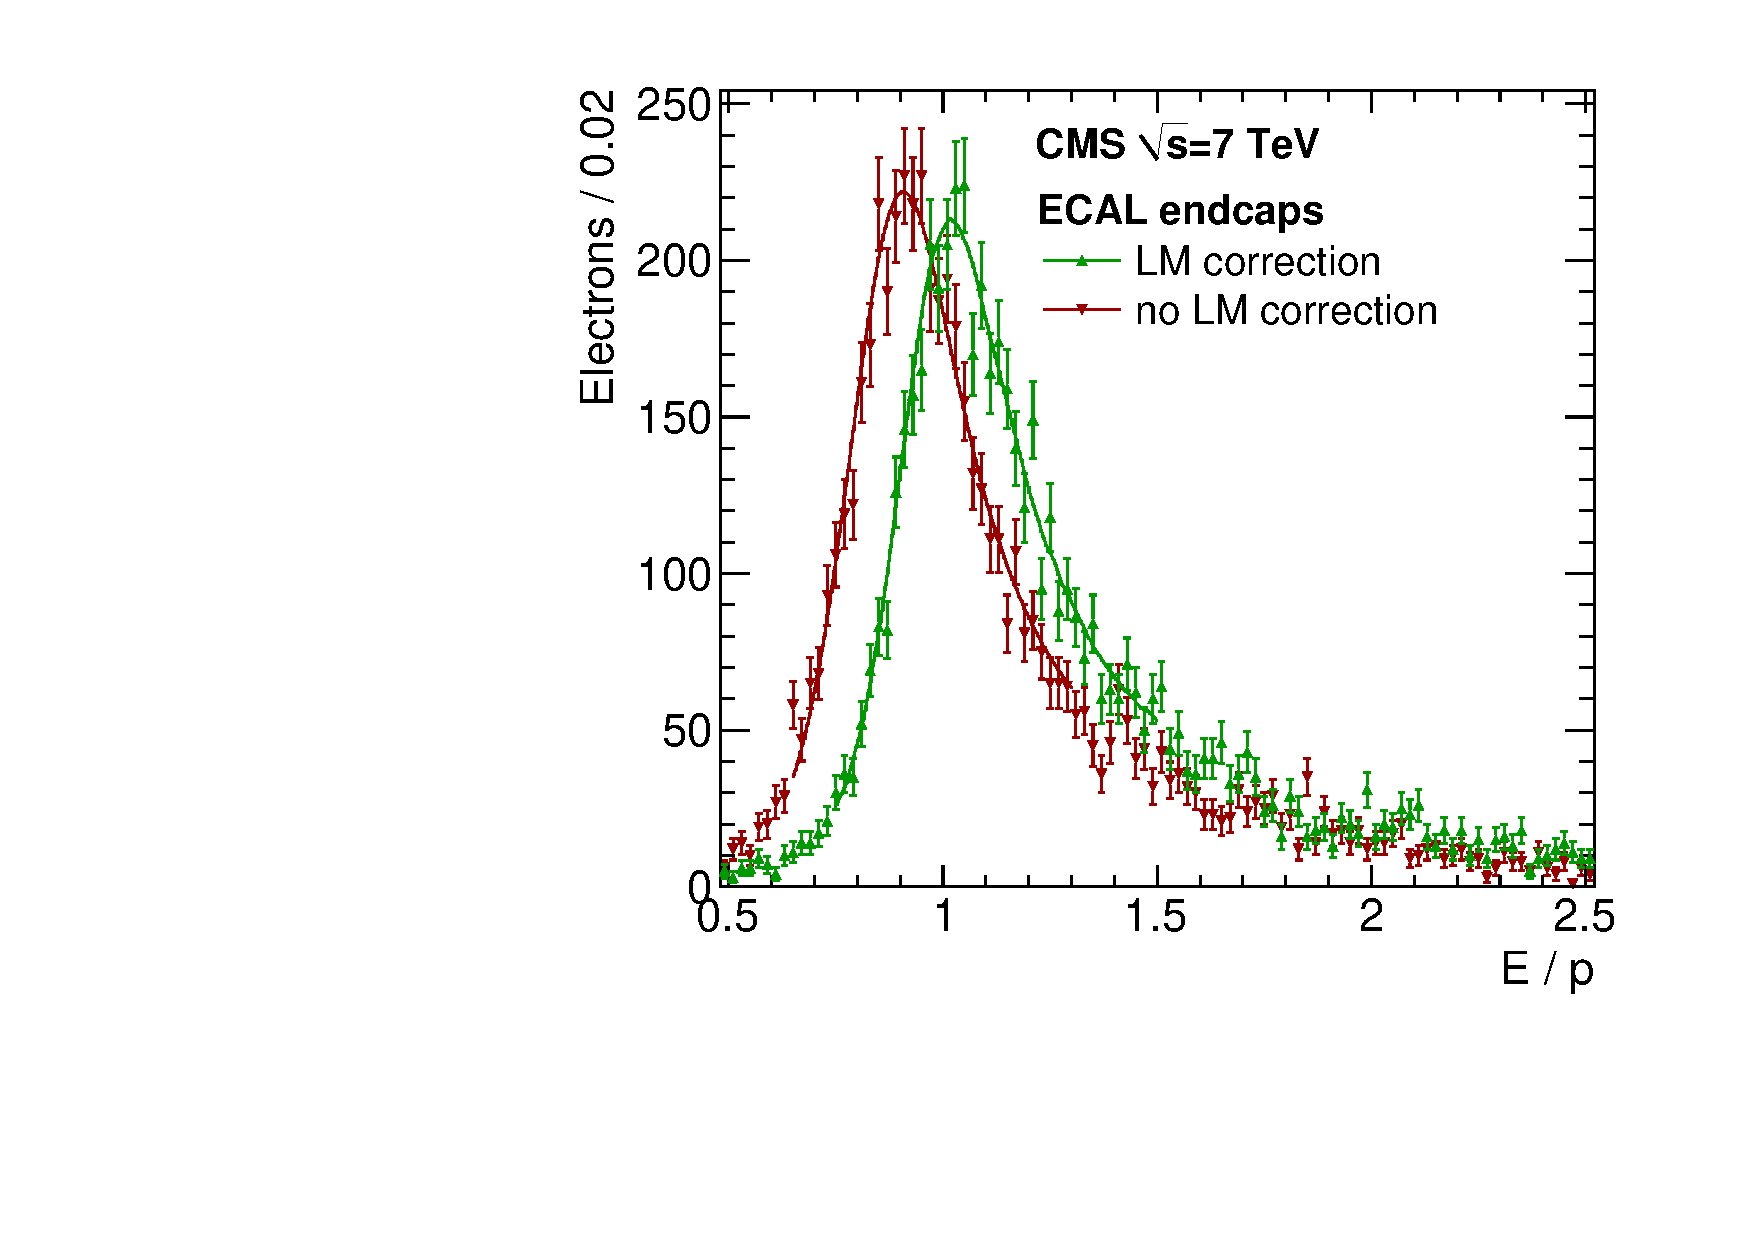
\includegraphics[width=0.40\linewidth]{figs/cms/EoP_TypicalFit_EE.pdf} &
 \hspace{-1cm}
 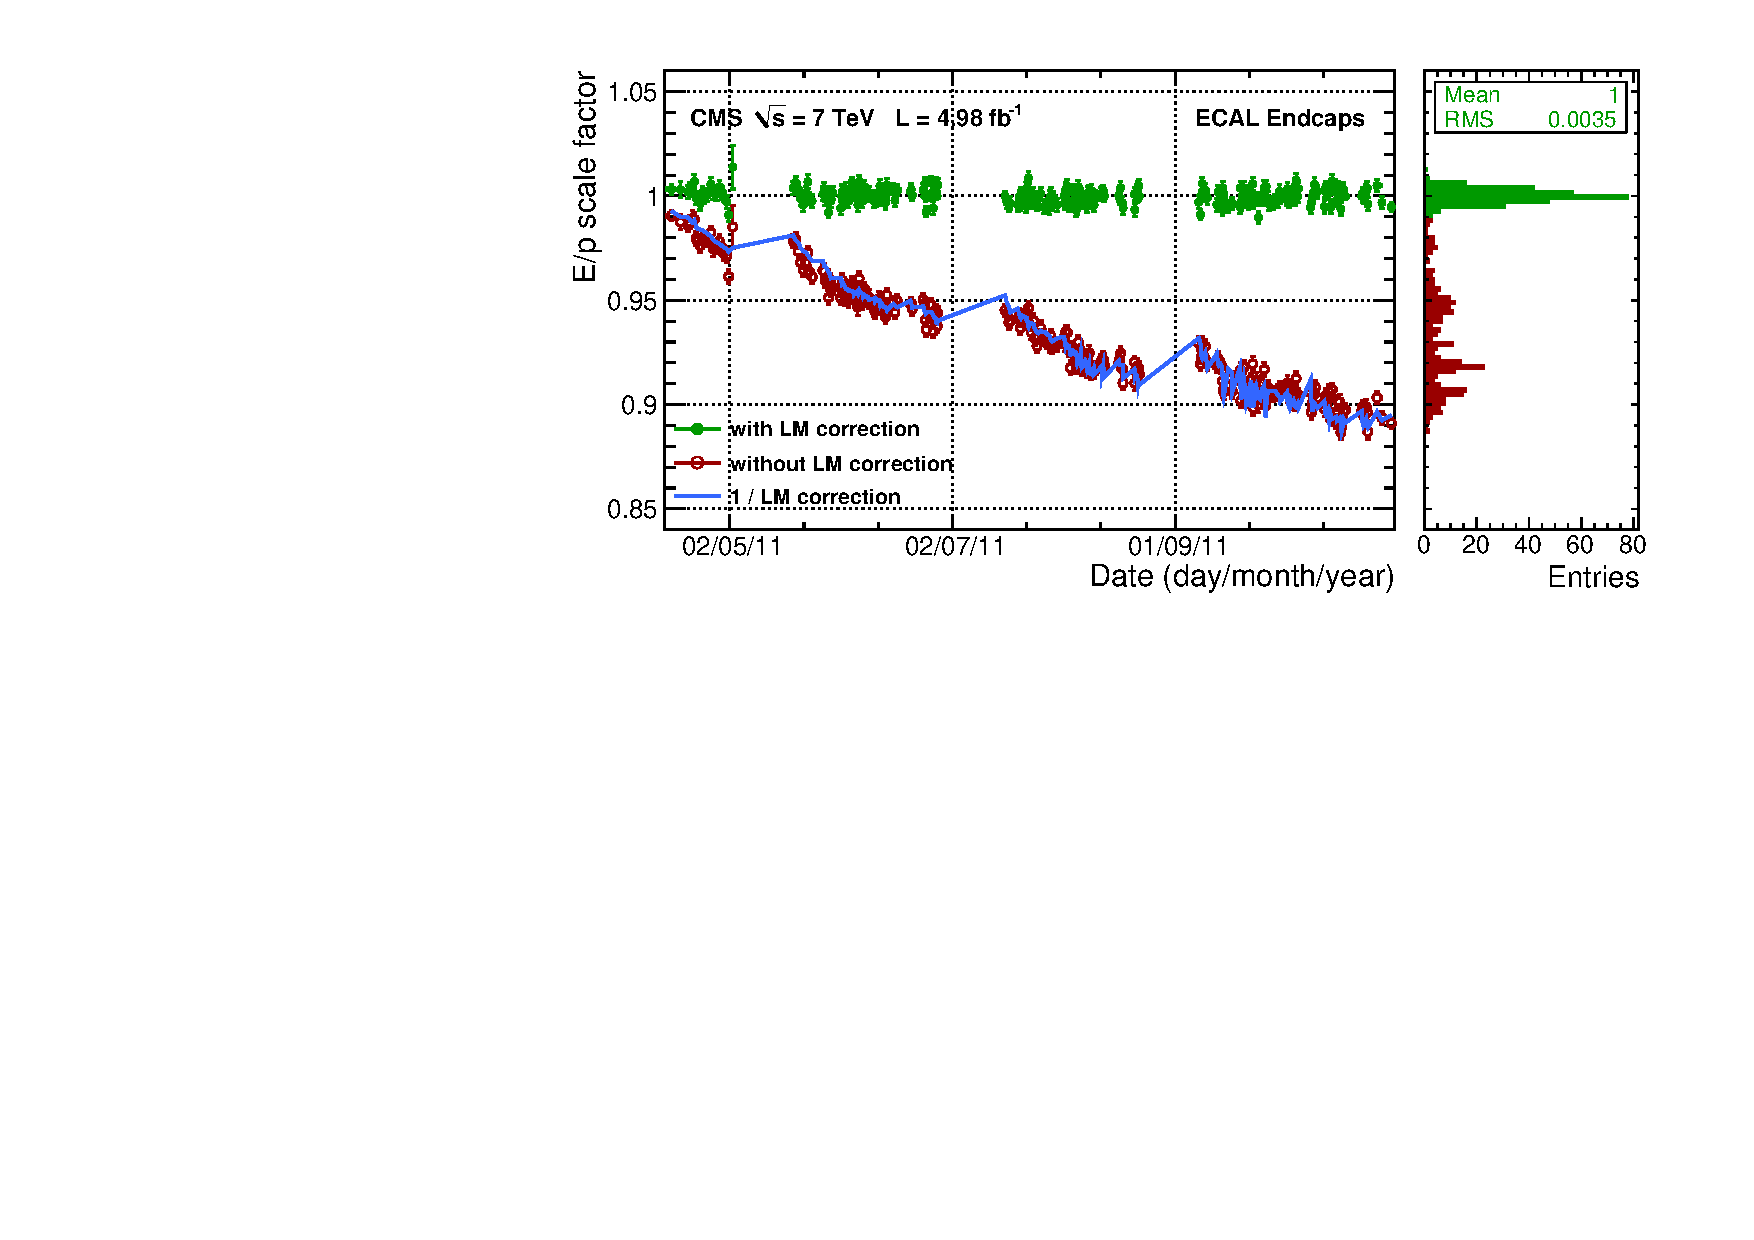
\includegraphics[width=0.69\linewidth]{figs/cms/EsuPhistoryEE_alpha116.pdf}
\end{tabular}
\end{center}
\caption{\label{fig:wenuEB}
Relative energy response variation for the barrel (top) and the endcaps (bottom)
determined from the $E/p$ analysis of electrons in $\PW$-boson decays.
Left: examples of fits to the $E/p$ distributions before (red) and
after (green) laser corrections. Middle: Response stability during the
2011 $\Pp\Pp$ data-taking period before (red open circles) and after
(green points) response corrections; the blue line shows the inverse
of the average laser corrections. Right: Distribution of the projected
relative energy scales.}
\end{figure}